\documentclass[twoside]{book}

% Packages required by doxygen
\usepackage{fixltx2e}
\usepackage{calc}
\usepackage{doxygen}
\usepackage[export]{adjustbox} % also loads graphicx
\usepackage{graphicx}
\usepackage[utf8]{inputenc}
\usepackage{makeidx}
\usepackage{multicol}
\usepackage{multirow}
\PassOptionsToPackage{warn}{textcomp}
\usepackage{textcomp}
\usepackage[nointegrals]{wasysym}
\usepackage[table]{xcolor}

% Font selection
\usepackage[T1]{fontenc}
\usepackage[scaled=.90]{helvet}
\usepackage{courier}
\usepackage{amssymb}
\usepackage{sectsty}
\renewcommand{\familydefault}{\sfdefault}
\allsectionsfont{%
  \fontseries{bc}\selectfont%
  \color{darkgray}%
}
\renewcommand{\DoxyLabelFont}{%
  \fontseries{bc}\selectfont%
  \color{darkgray}%
}
\newcommand{\+}{\discretionary{\mbox{\scriptsize$\hookleftarrow$}}{}{}}

% Page & text layout
\usepackage{geometry}
\geometry{%
  a4paper,%
  top=2.5cm,%
  bottom=2.5cm,%
  left=2.5cm,%
  right=2.5cm%
}
\tolerance=750
\hfuzz=15pt
\hbadness=750
\setlength{\emergencystretch}{15pt}
\setlength{\parindent}{0cm}
\setlength{\parskip}{3ex plus 2ex minus 2ex}
\makeatletter
\renewcommand{\paragraph}{%
  \@startsection{paragraph}{4}{0ex}{-1.0ex}{1.0ex}{%
    \normalfont\normalsize\bfseries\SS@parafont%
  }%
}
\renewcommand{\subparagraph}{%
  \@startsection{subparagraph}{5}{0ex}{-1.0ex}{1.0ex}{%
    \normalfont\normalsize\bfseries\SS@subparafont%
  }%
}
\makeatother

% Headers & footers
\usepackage{fancyhdr}
\pagestyle{fancyplain}
\fancyhead[LE]{\fancyplain{}{\bfseries\thepage}}
\fancyhead[CE]{\fancyplain{}{}}
\fancyhead[RE]{\fancyplain{}{\bfseries\leftmark}}
\fancyhead[LO]{\fancyplain{}{\bfseries\rightmark}}
\fancyhead[CO]{\fancyplain{}{}}
\fancyhead[RO]{\fancyplain{}{\bfseries\thepage}}
\fancyfoot[LE]{\fancyplain{}{}}
\fancyfoot[CE]{\fancyplain{}{}}
\fancyfoot[RE]{\fancyplain{}{\bfseries\scriptsize Generated by Doxygen }}
\fancyfoot[LO]{\fancyplain{}{\bfseries\scriptsize Generated by Doxygen }}
\fancyfoot[CO]{\fancyplain{}{}}
\fancyfoot[RO]{\fancyplain{}{}}
\renewcommand{\footrulewidth}{0.4pt}
\renewcommand{\chaptermark}[1]{%
  \markboth{#1}{}%
}
\renewcommand{\sectionmark}[1]{%
  \markright{\thesection\ #1}%
}

% Indices & bibliography
\usepackage{natbib}
\usepackage[titles]{tocloft}
\setcounter{tocdepth}{3}
\setcounter{secnumdepth}{5}
\makeindex

% Hyperlinks (required, but should be loaded last)
\usepackage{ifpdf}
\ifpdf
  \usepackage[pdftex,pagebackref=true]{hyperref}
\else
  \usepackage[ps2pdf,pagebackref=true]{hyperref}
\fi
\hypersetup{%
  colorlinks=true,%
  linkcolor=blue,%
  citecolor=blue,%
  unicode%
}

% Custom commands
\newcommand{\clearemptydoublepage}{%
  \newpage{\pagestyle{empty}\cleardoublepage}%
}

\usepackage{caption}
\captionsetup{labelsep=space,justification=centering,font={bf},singlelinecheck=off,skip=4pt,position=top}

%===== C O N T E N T S =====

\begin{document}

% Titlepage & ToC
\hypersetup{pageanchor=false,
             bookmarksnumbered=true,
             pdfencoding=unicode
            }
\pagenumbering{alph}
\begin{titlepage}
\vspace*{7cm}
\begin{center}%
{\Large Chess }\\
\vspace*{1cm}
{\large Generated by Doxygen 1.8.12}\\
\end{center}
\end{titlepage}
\clearemptydoublepage
\pagenumbering{roman}
\tableofcontents
\clearemptydoublepage
\pagenumbering{arabic}
\hypersetup{pageanchor=true}

%--- Begin generated contents ---
\chapter{Hierarchical Index}
\section{Class Hierarchy}
This inheritance list is sorted roughly, but not completely, alphabetically\+:\begin{DoxyCompactList}
\item \contentsline{section}{tests.\+pieces.\+All\+Piece\+Tests}{\pageref{classtests_1_1pieces_1_1_all_piece_tests}}{}
\item \contentsline{section}{tests.\+pieces.\+Bishop\+Test}{\pageref{classtests_1_1pieces_1_1_bishop_test}}{}
\item \contentsline{section}{main.\+model.\+Board}{\pageref{classmain_1_1model_1_1_board}}{}
\item \contentsline{section}{tests.\+game.\+Board\+Test}{\pageref{classtests_1_1game_1_1_board_test}}{}
\item \contentsline{section}{main.\+Board\+View}{\pageref{classmain_1_1_board_view}}{}
\item \contentsline{section}{tests.\+Common}{\pageref{classtests_1_1_common}}{}
\item Comparable\begin{DoxyCompactList}
\item \contentsline{section}{main.\+model.\+Coordinate}{\pageref{classmain_1_1model_1_1_coordinate}}{}
\end{DoxyCompactList}
\item \contentsline{section}{main.\+Constants}{\pageref{classmain_1_1_constants}}{}
\item \contentsline{section}{tests.\+pieces.\+Ferz\+Test}{\pageref{classtests_1_1pieces_1_1_ferz_test}}{}
\item \contentsline{section}{main.\+Game\+Controller}{\pageref{classmain_1_1_game_controller}}{}
\item \contentsline{section}{main.\+model.\+Initializer}{\pageref{classmain_1_1model_1_1_initializer}}{}
\item \contentsline{section}{tests.\+pieces.\+King\+Test}{\pageref{classtests_1_1pieces_1_1_king_test}}{}
\item \contentsline{section}{tests.\+pieces.\+Knight\+Test}{\pageref{classtests_1_1pieces_1_1_knight_test}}{}
\item \contentsline{section}{main.\+model.\+Move}{\pageref{classmain_1_1model_1_1_move}}{}
\item \contentsline{section}{tests.\+pieces.\+Pawn\+Test}{\pageref{classtests_1_1pieces_1_1_pawn_test}}{}
\item \contentsline{section}{main.\+pieces.\+Piece}{\pageref{classmain_1_1pieces_1_1_piece}}{}
\begin{DoxyCompactList}
\item \contentsline{section}{main.\+pieces.\+Bishop}{\pageref{classmain_1_1pieces_1_1_bishop}}{}
\item \contentsline{section}{main.\+pieces.\+Ferz}{\pageref{classmain_1_1pieces_1_1_ferz}}{}
\item \contentsline{section}{main.\+pieces.\+King}{\pageref{classmain_1_1pieces_1_1_king}}{}
\item \contentsline{section}{main.\+pieces.\+Knight}{\pageref{classmain_1_1pieces_1_1_knight}}{}
\item \contentsline{section}{main.\+pieces.\+Pawn}{\pageref{classmain_1_1pieces_1_1_pawn}}{}
\item \contentsline{section}{main.\+pieces.\+Princess}{\pageref{classmain_1_1pieces_1_1_princess}}{}
\item \contentsline{section}{main.\+pieces.\+Queen}{\pageref{classmain_1_1pieces_1_1_queen}}{}
\item \contentsline{section}{main.\+pieces.\+Rook}{\pageref{classmain_1_1pieces_1_1_rook}}{}
\end{DoxyCompactList}
\item \contentsline{section}{tests.\+pieces.\+Piece\+Test}{\pageref{classtests_1_1pieces_1_1_piece_test}}{}
\item \contentsline{section}{main.\+Player}{\pageref{classmain_1_1_player}}{}
\item \contentsline{section}{tests.\+game.\+Player\+Test}{\pageref{classtests_1_1game_1_1_player_test}}{}
\item \contentsline{section}{tests.\+pieces.\+Princess\+Test}{\pageref{classtests_1_1pieces_1_1_princess_test}}{}
\item \contentsline{section}{tests.\+pieces.\+Queen\+Test}{\pageref{classtests_1_1pieces_1_1_queen_test}}{}
\item \contentsline{section}{tests.\+pieces.\+Rook\+Test}{\pageref{classtests_1_1pieces_1_1_rook_test}}{}
\item Test\+Suite\begin{DoxyCompactList}
\item \contentsline{section}{tests.\+Run\+All\+Tests}{\pageref{classtests_1_1_run_all_tests}}{}
\end{DoxyCompactList}
\end{DoxyCompactList}

\chapter{Class Index}
\section{Class List}
Here are the classes, structs, unions and interfaces with brief descriptions\+:\begin{DoxyCompactList}
\item\contentsline{section}{\hyperlink{classtests_1_1pieces_1_1_all_piece_tests}{tests.\+pieces.\+All\+Piece\+Tests} }{\pageref{classtests_1_1pieces_1_1_all_piece_tests}}{}
\item\contentsline{section}{\hyperlink{classmain_1_1pieces_1_1_bishop}{main.\+pieces.\+Bishop} }{\pageref{classmain_1_1pieces_1_1_bishop}}{}
\item\contentsline{section}{\hyperlink{classtests_1_1pieces_1_1_bishop_test}{tests.\+pieces.\+Bishop\+Test} }{\pageref{classtests_1_1pieces_1_1_bishop_test}}{}
\item\contentsline{section}{\hyperlink{classmain_1_1model_1_1_board}{main.\+model.\+Board} }{\pageref{classmain_1_1model_1_1_board}}{}
\item\contentsline{section}{\hyperlink{classtests_1_1game_1_1_board_test}{tests.\+game.\+Board\+Test} }{\pageref{classtests_1_1game_1_1_board_test}}{}
\item\contentsline{section}{\hyperlink{classmain_1_1_board_view}{main.\+Board\+View} }{\pageref{classmain_1_1_board_view}}{}
\item\contentsline{section}{\hyperlink{classtests_1_1_common}{tests.\+Common} }{\pageref{classtests_1_1_common}}{}
\item\contentsline{section}{\hyperlink{classmain_1_1_constants}{main.\+Constants} }{\pageref{classmain_1_1_constants}}{}
\item\contentsline{section}{\hyperlink{classmain_1_1model_1_1_coordinate}{main.\+model.\+Coordinate} }{\pageref{classmain_1_1model_1_1_coordinate}}{}
\item\contentsline{section}{\hyperlink{classmain_1_1pieces_1_1_ferz}{main.\+pieces.\+Ferz} }{\pageref{classmain_1_1pieces_1_1_ferz}}{}
\item\contentsline{section}{\hyperlink{classtests_1_1pieces_1_1_ferz_test}{tests.\+pieces.\+Ferz\+Test} }{\pageref{classtests_1_1pieces_1_1_ferz_test}}{}
\item\contentsline{section}{\hyperlink{classmain_1_1_game_controller}{main.\+Game\+Controller} }{\pageref{classmain_1_1_game_controller}}{}
\item\contentsline{section}{\hyperlink{classmain_1_1model_1_1_initializer}{main.\+model.\+Initializer} }{\pageref{classmain_1_1model_1_1_initializer}}{}
\item\contentsline{section}{\hyperlink{classmain_1_1pieces_1_1_king}{main.\+pieces.\+King} }{\pageref{classmain_1_1pieces_1_1_king}}{}
\item\contentsline{section}{\hyperlink{classtests_1_1pieces_1_1_king_test}{tests.\+pieces.\+King\+Test} }{\pageref{classtests_1_1pieces_1_1_king_test}}{}
\item\contentsline{section}{\hyperlink{classmain_1_1pieces_1_1_knight}{main.\+pieces.\+Knight} }{\pageref{classmain_1_1pieces_1_1_knight}}{}
\item\contentsline{section}{\hyperlink{classtests_1_1pieces_1_1_knight_test}{tests.\+pieces.\+Knight\+Test} }{\pageref{classtests_1_1pieces_1_1_knight_test}}{}
\item\contentsline{section}{\hyperlink{classmain_1_1model_1_1_move}{main.\+model.\+Move} }{\pageref{classmain_1_1model_1_1_move}}{}
\item\contentsline{section}{\hyperlink{classmain_1_1pieces_1_1_pawn}{main.\+pieces.\+Pawn} }{\pageref{classmain_1_1pieces_1_1_pawn}}{}
\item\contentsline{section}{\hyperlink{classtests_1_1pieces_1_1_pawn_test}{tests.\+pieces.\+Pawn\+Test} }{\pageref{classtests_1_1pieces_1_1_pawn_test}}{}
\item\contentsline{section}{\hyperlink{classmain_1_1pieces_1_1_piece}{main.\+pieces.\+Piece} }{\pageref{classmain_1_1pieces_1_1_piece}}{}
\item\contentsline{section}{\hyperlink{classtests_1_1pieces_1_1_piece_test}{tests.\+pieces.\+Piece\+Test} }{\pageref{classtests_1_1pieces_1_1_piece_test}}{}
\item\contentsline{section}{\hyperlink{classmain_1_1_player}{main.\+Player} }{\pageref{classmain_1_1_player}}{}
\item\contentsline{section}{\hyperlink{classtests_1_1game_1_1_player_test}{tests.\+game.\+Player\+Test} }{\pageref{classtests_1_1game_1_1_player_test}}{}
\item\contentsline{section}{\hyperlink{classmain_1_1pieces_1_1_princess}{main.\+pieces.\+Princess} }{\pageref{classmain_1_1pieces_1_1_princess}}{}
\item\contentsline{section}{\hyperlink{classtests_1_1pieces_1_1_princess_test}{tests.\+pieces.\+Princess\+Test} }{\pageref{classtests_1_1pieces_1_1_princess_test}}{}
\item\contentsline{section}{\hyperlink{classmain_1_1pieces_1_1_queen}{main.\+pieces.\+Queen} }{\pageref{classmain_1_1pieces_1_1_queen}}{}
\item\contentsline{section}{\hyperlink{classtests_1_1pieces_1_1_queen_test}{tests.\+pieces.\+Queen\+Test} }{\pageref{classtests_1_1pieces_1_1_queen_test}}{}
\item\contentsline{section}{\hyperlink{classmain_1_1pieces_1_1_rook}{main.\+pieces.\+Rook} }{\pageref{classmain_1_1pieces_1_1_rook}}{}
\item\contentsline{section}{\hyperlink{classtests_1_1pieces_1_1_rook_test}{tests.\+pieces.\+Rook\+Test} }{\pageref{classtests_1_1pieces_1_1_rook_test}}{}
\item\contentsline{section}{\hyperlink{classtests_1_1_run_all_tests}{tests.\+Run\+All\+Tests} }{\pageref{classtests_1_1_run_all_tests}}{}
\end{DoxyCompactList}

\chapter{Class Documentation}
\hypertarget{classtests_1_1pieces_1_1_all_piece_tests}{}\section{tests.\+pieces.\+All\+Piece\+Tests Class Reference}
\label{classtests_1_1pieces_1_1_all_piece_tests}\index{tests.\+pieces.\+All\+Piece\+Tests@{tests.\+pieces.\+All\+Piece\+Tests}}


\subsection{Detailed Description}
Created by samir on 9/7/16. 

The documentation for this class was generated from the following file\+:\begin{DoxyCompactItemize}
\item 
src/tests/pieces/All\+Piece\+Tests.\+java\end{DoxyCompactItemize}

\hypertarget{classmain_1_1pieces_1_1_bishop}{}\section{main.\+pieces.\+Bishop Class Reference}
\label{classmain_1_1pieces_1_1_bishop}\index{main.\+pieces.\+Bishop@{main.\+pieces.\+Bishop}}
Inheritance diagram for main.\+pieces.\+Bishop\+:\begin{figure}[H]
\begin{center}
\leavevmode
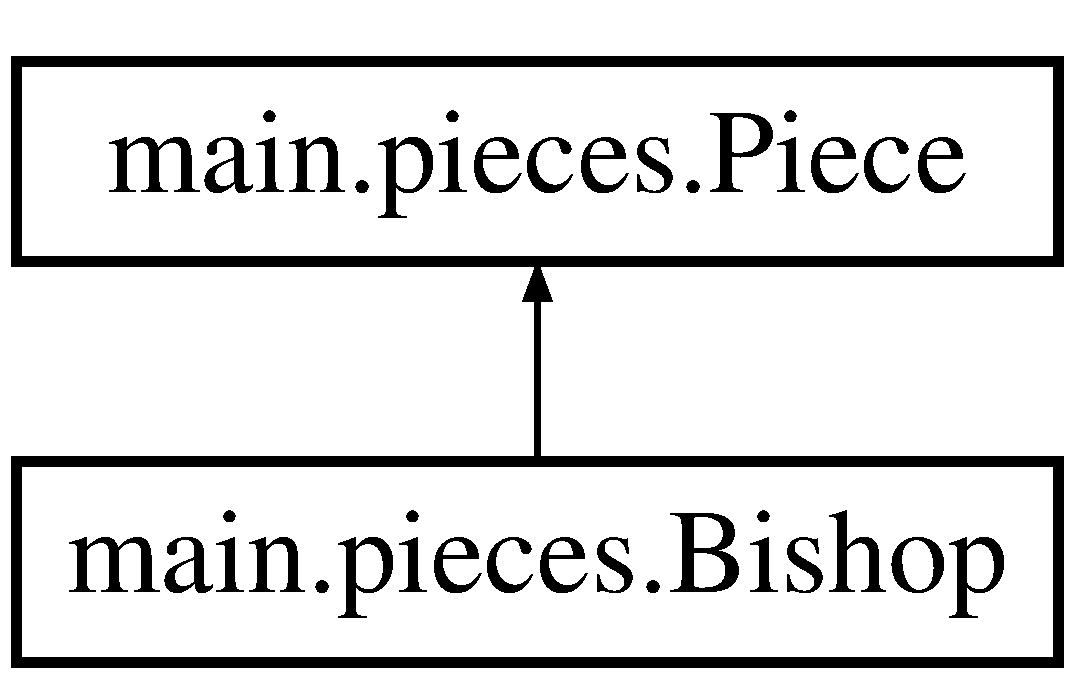
\includegraphics[height=2.000000cm]{classmain_1_1pieces_1_1_bishop}
\end{center}
\end{figure}
\subsection*{Public Member Functions}
\begin{DoxyCompactItemize}
\item 
\hyperlink{classmain_1_1pieces_1_1_bishop_a14dd49999f0dd6d0d8fb96d9c09fbd8b}{Bishop} (String color)
\item 
String \hyperlink{classmain_1_1pieces_1_1_bishop_a6621662a277c0a45fb317b7d37612410}{to\+String} ()
\item 
String \hyperlink{classmain_1_1pieces_1_1_bishop_a99e4744c895f53d2d9c46c83a77be273}{get\+Type} ()
\item 
Array\+List$<$ \hyperlink{classmain_1_1model_1_1_coordinate}{Coordinate} $>$ \hyperlink{classmain_1_1pieces_1_1_bishop_a9abb24030574df6017a2f994125c5959}{possible\+Moves} ()
\end{DoxyCompactItemize}
\subsection*{Additional Inherited Members}


\subsection{Detailed Description}
Created by samir on 9/3/16. 

\subsection{Constructor \& Destructor Documentation}
\hypertarget{classmain_1_1pieces_1_1_bishop_a14dd49999f0dd6d0d8fb96d9c09fbd8b}{}\label{classmain_1_1pieces_1_1_bishop_a14dd49999f0dd6d0d8fb96d9c09fbd8b} 
\index{main\+::pieces\+::\+Bishop@{main\+::pieces\+::\+Bishop}!Bishop@{Bishop}}
\index{Bishop@{Bishop}!main\+::pieces\+::\+Bishop@{main\+::pieces\+::\+Bishop}}
\subsubsection{\texorpdfstring{Bishop()}{Bishop()}}
{\footnotesize\ttfamily main.\+pieces.\+Bishop.\+Bishop (\begin{DoxyParamCaption}\item[{String}]{color }\end{DoxyParamCaption})}

Constructor taking in an x and y coordinate 

\subsection{Member Function Documentation}
\hypertarget{classmain_1_1pieces_1_1_bishop_a99e4744c895f53d2d9c46c83a77be273}{}\label{classmain_1_1pieces_1_1_bishop_a99e4744c895f53d2d9c46c83a77be273} 
\index{main\+::pieces\+::\+Bishop@{main\+::pieces\+::\+Bishop}!get\+Type@{get\+Type}}
\index{get\+Type@{get\+Type}!main\+::pieces\+::\+Bishop@{main\+::pieces\+::\+Bishop}}
\subsubsection{\texorpdfstring{get\+Type()}{getType()}}
{\footnotesize\ttfamily String main.\+pieces.\+Bishop.\+get\+Type (\begin{DoxyParamCaption}{ }\end{DoxyParamCaption})}

Returns the type of this piece \hypertarget{classmain_1_1pieces_1_1_bishop_a9abb24030574df6017a2f994125c5959}{}\label{classmain_1_1pieces_1_1_bishop_a9abb24030574df6017a2f994125c5959} 
\index{main\+::pieces\+::\+Bishop@{main\+::pieces\+::\+Bishop}!possible\+Moves@{possible\+Moves}}
\index{possible\+Moves@{possible\+Moves}!main\+::pieces\+::\+Bishop@{main\+::pieces\+::\+Bishop}}
\subsubsection{\texorpdfstring{possible\+Moves()}{possibleMoves()}}
{\footnotesize\ttfamily Array\+List$<$\hyperlink{classmain_1_1model_1_1_coordinate}{Coordinate}$>$ main.\+pieces.\+Bishop.\+possible\+Moves (\begin{DoxyParamCaption}{ }\end{DoxyParamCaption})}

Return the list of possible legal moves the bishop can make \begin{DoxyReturn}{Returns}

\end{DoxyReturn}
\hypertarget{classmain_1_1pieces_1_1_bishop_a6621662a277c0a45fb317b7d37612410}{}\label{classmain_1_1pieces_1_1_bishop_a6621662a277c0a45fb317b7d37612410} 
\index{main\+::pieces\+::\+Bishop@{main\+::pieces\+::\+Bishop}!to\+String@{to\+String}}
\index{to\+String@{to\+String}!main\+::pieces\+::\+Bishop@{main\+::pieces\+::\+Bishop}}
\subsubsection{\texorpdfstring{to\+String()}{toString()}}
{\footnotesize\ttfamily String main.\+pieces.\+Bishop.\+to\+String (\begin{DoxyParamCaption}{ }\end{DoxyParamCaption})}

String representation of a \hyperlink{classmain_1_1pieces_1_1_rook}{Rook} \begin{DoxyReturn}{Returns}

\end{DoxyReturn}


The documentation for this class was generated from the following file\+:\begin{DoxyCompactItemize}
\item 
src/main/pieces/Bishop.\+java\end{DoxyCompactItemize}

\hypertarget{classtests_1_1pieces_1_1_bishop_test}{}\section{tests.\+pieces.\+Bishop\+Test Class Reference}
\label{classtests_1_1pieces_1_1_bishop_test}\index{tests.\+pieces.\+Bishop\+Test@{tests.\+pieces.\+Bishop\+Test}}
\subsection*{Public Member Functions}
\begin{DoxyCompactItemize}
\item 
void \hyperlink{classtests_1_1pieces_1_1_bishop_test_a56e8b7b1d2be0b154ce7a51b3c2851a6}{valid\+Bishop\+Constructor} ()  throws Exception 
\item 
void \hyperlink{classtests_1_1pieces_1_1_bishop_test_a8237167f486fa797b996b55c726ad9cc}{valid\+Bishop\+Movement} ()  throws Exception 
\item 
void \hyperlink{classtests_1_1pieces_1_1_bishop_test_aad795e069e5b506f723c44d7b31fc794}{invalid\+Bishop\+Movement} ()  throws Exception 
\end{DoxyCompactItemize}


\subsection{Detailed Description}
Created by samir on 9/4/16. 

\subsection{Member Function Documentation}
\hypertarget{classtests_1_1pieces_1_1_bishop_test_aad795e069e5b506f723c44d7b31fc794}{}\label{classtests_1_1pieces_1_1_bishop_test_aad795e069e5b506f723c44d7b31fc794} 
\index{tests\+::pieces\+::\+Bishop\+Test@{tests\+::pieces\+::\+Bishop\+Test}!invalid\+Bishop\+Movement@{invalid\+Bishop\+Movement}}
\index{invalid\+Bishop\+Movement@{invalid\+Bishop\+Movement}!tests\+::pieces\+::\+Bishop\+Test@{tests\+::pieces\+::\+Bishop\+Test}}
\subsubsection{\texorpdfstring{invalid\+Bishop\+Movement()}{invalidBishopMovement()}}
{\footnotesize\ttfamily void tests.\+pieces.\+Bishop\+Test.\+invalid\+Bishop\+Movement (\begin{DoxyParamCaption}{ }\end{DoxyParamCaption}) throws Exception}

Test for invalid bishop movement (no available moves at start) \hypertarget{classtests_1_1pieces_1_1_bishop_test_a56e8b7b1d2be0b154ce7a51b3c2851a6}{}\label{classtests_1_1pieces_1_1_bishop_test_a56e8b7b1d2be0b154ce7a51b3c2851a6} 
\index{tests\+::pieces\+::\+Bishop\+Test@{tests\+::pieces\+::\+Bishop\+Test}!valid\+Bishop\+Constructor@{valid\+Bishop\+Constructor}}
\index{valid\+Bishop\+Constructor@{valid\+Bishop\+Constructor}!tests\+::pieces\+::\+Bishop\+Test@{tests\+::pieces\+::\+Bishop\+Test}}
\subsubsection{\texorpdfstring{valid\+Bishop\+Constructor()}{validBishopConstructor()}}
{\footnotesize\ttfamily void tests.\+pieces.\+Bishop\+Test.\+valid\+Bishop\+Constructor (\begin{DoxyParamCaption}{ }\end{DoxyParamCaption}) throws Exception}

Valid constructor for a bishop should not throw an exception \hypertarget{classtests_1_1pieces_1_1_bishop_test_a8237167f486fa797b996b55c726ad9cc}{}\label{classtests_1_1pieces_1_1_bishop_test_a8237167f486fa797b996b55c726ad9cc} 
\index{tests\+::pieces\+::\+Bishop\+Test@{tests\+::pieces\+::\+Bishop\+Test}!valid\+Bishop\+Movement@{valid\+Bishop\+Movement}}
\index{valid\+Bishop\+Movement@{valid\+Bishop\+Movement}!tests\+::pieces\+::\+Bishop\+Test@{tests\+::pieces\+::\+Bishop\+Test}}
\subsubsection{\texorpdfstring{valid\+Bishop\+Movement()}{validBishopMovement()}}
{\footnotesize\ttfamily void tests.\+pieces.\+Bishop\+Test.\+valid\+Bishop\+Movement (\begin{DoxyParamCaption}{ }\end{DoxyParamCaption}) throws Exception}

Test for valid bishop movement (should be able to move) Check the valid moves match up 
\begin{DoxyExceptions}{Exceptions}
{\em Exception} & \\
\hline
\end{DoxyExceptions}


The documentation for this class was generated from the following file\+:\begin{DoxyCompactItemize}
\item 
src/tests/pieces/Bishop\+Test.\+java\end{DoxyCompactItemize}

\hypertarget{classmain_1_1model_1_1_board}{}\section{main.\+model.\+Board Class Reference}
\label{classmain_1_1model_1_1_board}\index{main.\+model.\+Board@{main.\+model.\+Board}}
\subsection*{Public Member Functions}
\begin{DoxyCompactItemize}
\item 
\hyperlink{classmain_1_1model_1_1_board_aa960cea7bc44db0fdb54d18767579c52}{Board} (int length, int width)
\item 
\hyperlink{classmain_1_1model_1_1_board_a96612d9907fdc7144072b39701f3c98f}{Board} (int length, int width, String stalemate)
\item 
\hyperlink{classmain_1_1pieces_1_1_piece}{Piece} \hyperlink{classmain_1_1model_1_1_board_a58b12960567f10637634a020d9bc7ed6}{get\+King} (String color)
\item 
void \hyperlink{classmain_1_1model_1_1_board_ac89ac2b16c2e7ed3e0ff9160b471d99c}{set\+Piece} (\hyperlink{classmain_1_1pieces_1_1_piece}{Piece} piece, \hyperlink{classmain_1_1model_1_1_coordinate}{Coordinate} coordinate)
\item 
void \hyperlink{classmain_1_1model_1_1_board_a410cd03e774ce09fce169f8b047e413a}{set\+Piece} (\hyperlink{classmain_1_1pieces_1_1_piece}{Piece} piece, int x, int y)
\item 
void \hyperlink{classmain_1_1model_1_1_board_a267a2fd3d08cb25c4d35ceb9c61e5402}{remove\+Piece} (\hyperlink{classmain_1_1pieces_1_1_piece}{Piece} piece)
\item 
boolean \hyperlink{classmain_1_1model_1_1_board_a8924f9087f10a4554958ac48480e9b0b}{move\+Piece} (\hyperlink{classmain_1_1pieces_1_1_piece}{Piece} piece, \hyperlink{classmain_1_1model_1_1_coordinate}{Coordinate} coordinate)
\item 
\hyperlink{classmain_1_1pieces_1_1_piece}{Piece} \hyperlink{classmain_1_1model_1_1_board_abf3eb07b33b96a983bd98c26e7390ed4}{move\+Piece\+To\+Coordinate} (\hyperlink{classmain_1_1pieces_1_1_piece}{Piece} piece, \hyperlink{classmain_1_1model_1_1_coordinate}{Coordinate} coordinate)
\item 
boolean \hyperlink{classmain_1_1model_1_1_board_ac9396eab4affaccf9b66331a98f6e0d1}{is\+In\+Check} (String color)
\item 
void \hyperlink{classmain_1_1model_1_1_board_a6d983017a927def6bf7263b8a50c293a}{undo\+Move} (\hyperlink{classmain_1_1pieces_1_1_piece}{Piece} piece, \hyperlink{classmain_1_1pieces_1_1_piece}{Piece} existing, \hyperlink{classmain_1_1model_1_1_coordinate}{Coordinate} start, \hyperlink{classmain_1_1model_1_1_coordinate}{Coordinate} destination)
\item 
boolean \hyperlink{classmain_1_1model_1_1_board_abb5dfd9e2e597dd686351c1f06fbcb38}{is\+In\+Check\+Mate} (String color)
\item 
boolean \hyperlink{classmain_1_1model_1_1_board_aa3457acaf5b59679081273fc1e683be5}{has\+Any\+Moves} (String color)
\item 
boolean \hyperlink{classmain_1_1model_1_1_board_a6c144f940cc67d3f2f648f7fcc58294b}{is\+In\+Stalemate} (String color)
\item 
void \hyperlink{classmain_1_1model_1_1_board_ae838db532812c97d60e76ecd58027cc9}{print\+Board} ()
\item 
void \hyperlink{classmain_1_1model_1_1_board_ab822fe6d82c7951dbf950a6df4ee8b85}{initialize\+Piece} (String piece\+Type, int x, int y, String color)
\end{DoxyCompactItemize}
\subsection*{Static Public Member Functions}
\begin{DoxyCompactItemize}
\item 
\hypertarget{classmain_1_1model_1_1_board_a537a632327e7e27f10edcc2abe41de9f}{}\label{classmain_1_1model_1_1_board_a537a632327e7e27f10edcc2abe41de9f} 
static int {\bfseries get\+Length} ()
\item 
\hypertarget{classmain_1_1model_1_1_board_a00371e25d2973e637da7a768d1e2551a}{}\label{classmain_1_1model_1_1_board_a00371e25d2973e637da7a768d1e2551a} 
static int {\bfseries get\+Width} ()
\item 
static \hyperlink{classmain_1_1pieces_1_1_piece}{Piece} \hyperlink{classmain_1_1model_1_1_board_a9be517cf5bb1584069e14d202b4d708b}{get\+Piece} (int x, int y)
\item 
static \hyperlink{classmain_1_1pieces_1_1_piece}{Piece} \hyperlink{classmain_1_1model_1_1_board_acf3676f6e319705c9ed713d1c9fd097a}{get\+Piece} (\hyperlink{classmain_1_1model_1_1_coordinate}{Coordinate} coordinate)
\item 
static \hyperlink{classmain_1_1pieces_1_1_piece}{Piece} \mbox{[}$\,$\mbox{]}\mbox{[}$\,$\mbox{]} \hyperlink{classmain_1_1model_1_1_board_af7321b4ae3a390e48d3dd6c188de5d2e}{get\+Board} ()
\end{DoxyCompactItemize}


\subsection{Detailed Description}
Created by Samir on 9/1/16. 

\subsection{Constructor \& Destructor Documentation}
\hypertarget{classmain_1_1model_1_1_board_aa960cea7bc44db0fdb54d18767579c52}{}\label{classmain_1_1model_1_1_board_aa960cea7bc44db0fdb54d18767579c52} 
\index{main\+::model\+::\+Board@{main\+::model\+::\+Board}!Board@{Board}}
\index{Board@{Board}!main\+::model\+::\+Board@{main\+::model\+::\+Board}}
\subsubsection{\texorpdfstring{Board()}{Board()}\hspace{0.1cm}{\footnotesize\ttfamily [1/2]}}
{\footnotesize\ttfamily main.\+model.\+Board.\+Board (\begin{DoxyParamCaption}\item[{int}]{length,  }\item[{int}]{width }\end{DoxyParamCaption})}

Creates a board\+G\+UI with the dimensions of board\+Length and board\+Width \hypertarget{classmain_1_1model_1_1_board_a96612d9907fdc7144072b39701f3c98f}{}\label{classmain_1_1model_1_1_board_a96612d9907fdc7144072b39701f3c98f} 
\index{main\+::model\+::\+Board@{main\+::model\+::\+Board}!Board@{Board}}
\index{Board@{Board}!main\+::model\+::\+Board@{main\+::model\+::\+Board}}
\subsubsection{\texorpdfstring{Board()}{Board()}\hspace{0.1cm}{\footnotesize\ttfamily [2/2]}}
{\footnotesize\ttfamily main.\+model.\+Board.\+Board (\begin{DoxyParamCaption}\item[{int}]{length,  }\item[{int}]{width,  }\item[{String}]{stalemate }\end{DoxyParamCaption})}

Custom constructor (for testing) to construct a stalemate scenario 

\subsection{Member Function Documentation}
\hypertarget{classmain_1_1model_1_1_board_af7321b4ae3a390e48d3dd6c188de5d2e}{}\label{classmain_1_1model_1_1_board_af7321b4ae3a390e48d3dd6c188de5d2e} 
\index{main\+::model\+::\+Board@{main\+::model\+::\+Board}!get\+Board@{get\+Board}}
\index{get\+Board@{get\+Board}!main\+::model\+::\+Board@{main\+::model\+::\+Board}}
\subsubsection{\texorpdfstring{get\+Board()}{getBoard()}}
{\footnotesize\ttfamily static \hyperlink{classmain_1_1pieces_1_1_piece}{Piece} \mbox{[}$\,$\mbox{]}\mbox{[}$\,$\mbox{]} main.\+model.\+Board.\+get\+Board (\begin{DoxyParamCaption}{ }\end{DoxyParamCaption})\hspace{0.3cm}{\ttfamily [static]}}

\subparagraph*{}

\hyperlink{classmain_1_1model_1_1_board}{Board} Update Methods \subparagraph*{}

Returns the board\+G\+UI and piece locations \hypertarget{classmain_1_1model_1_1_board_a58b12960567f10637634a020d9bc7ed6}{}\label{classmain_1_1model_1_1_board_a58b12960567f10637634a020d9bc7ed6} 
\index{main\+::model\+::\+Board@{main\+::model\+::\+Board}!get\+King@{get\+King}}
\index{get\+King@{get\+King}!main\+::model\+::\+Board@{main\+::model\+::\+Board}}
\subsubsection{\texorpdfstring{get\+King()}{getKing()}}
{\footnotesize\ttfamily \hyperlink{classmain_1_1pieces_1_1_piece}{Piece} main.\+model.\+Board.\+get\+King (\begin{DoxyParamCaption}\item[{String}]{color }\end{DoxyParamCaption})}


\begin{DoxyParams}{Parameters}
{\em color} & \\
\hline
\end{DoxyParams}
\begin{DoxyReturn}{Returns}

\end{DoxyReturn}
\hypertarget{classmain_1_1model_1_1_board_a9be517cf5bb1584069e14d202b4d708b}{}\label{classmain_1_1model_1_1_board_a9be517cf5bb1584069e14d202b4d708b} 
\index{main\+::model\+::\+Board@{main\+::model\+::\+Board}!get\+Piece@{get\+Piece}}
\index{get\+Piece@{get\+Piece}!main\+::model\+::\+Board@{main\+::model\+::\+Board}}
\subsubsection{\texorpdfstring{get\+Piece()}{getPiece()}\hspace{0.1cm}{\footnotesize\ttfamily [1/2]}}
{\footnotesize\ttfamily static \hyperlink{classmain_1_1pieces_1_1_piece}{Piece} main.\+model.\+Board.\+get\+Piece (\begin{DoxyParamCaption}\item[{int}]{x,  }\item[{int}]{y }\end{DoxyParamCaption})\hspace{0.3cm}{\ttfamily [static]}}

Return the piece at the location given by x and y \hypertarget{classmain_1_1model_1_1_board_acf3676f6e319705c9ed713d1c9fd097a}{}\label{classmain_1_1model_1_1_board_acf3676f6e319705c9ed713d1c9fd097a} 
\index{main\+::model\+::\+Board@{main\+::model\+::\+Board}!get\+Piece@{get\+Piece}}
\index{get\+Piece@{get\+Piece}!main\+::model\+::\+Board@{main\+::model\+::\+Board}}
\subsubsection{\texorpdfstring{get\+Piece()}{getPiece()}\hspace{0.1cm}{\footnotesize\ttfamily [2/2]}}
{\footnotesize\ttfamily static \hyperlink{classmain_1_1pieces_1_1_piece}{Piece} main.\+model.\+Board.\+get\+Piece (\begin{DoxyParamCaption}\item[{\hyperlink{classmain_1_1model_1_1_coordinate}{Coordinate}}]{coordinate }\end{DoxyParamCaption})\hspace{0.3cm}{\ttfamily [static]}}

Return the piece at the corresponding coordinate \hypertarget{classmain_1_1model_1_1_board_aa3457acaf5b59679081273fc1e683be5}{}\label{classmain_1_1model_1_1_board_aa3457acaf5b59679081273fc1e683be5} 
\index{main\+::model\+::\+Board@{main\+::model\+::\+Board}!has\+Any\+Moves@{has\+Any\+Moves}}
\index{has\+Any\+Moves@{has\+Any\+Moves}!main\+::model\+::\+Board@{main\+::model\+::\+Board}}
\subsubsection{\texorpdfstring{has\+Any\+Moves()}{hasAnyMoves()}}
{\footnotesize\ttfamily boolean main.\+model.\+Board.\+has\+Any\+Moves (\begin{DoxyParamCaption}\item[{String}]{color }\end{DoxyParamCaption})}

Function to check if a player has any valid moves that they can make For all of their pieces, check if any piece can make a move without being in check 
\begin{DoxyParams}{Parameters}
{\em color} & \\
\hline
\end{DoxyParams}
\begin{DoxyReturn}{Returns}
True if they do, false if they don\textquotesingle{}t 
\end{DoxyReturn}
\hypertarget{classmain_1_1model_1_1_board_ab822fe6d82c7951dbf950a6df4ee8b85}{}\label{classmain_1_1model_1_1_board_ab822fe6d82c7951dbf950a6df4ee8b85} 
\index{main\+::model\+::\+Board@{main\+::model\+::\+Board}!initialize\+Piece@{initialize\+Piece}}
\index{initialize\+Piece@{initialize\+Piece}!main\+::model\+::\+Board@{main\+::model\+::\+Board}}
\subsubsection{\texorpdfstring{initialize\+Piece()}{initializePiece()}}
{\footnotesize\ttfamily void main.\+model.\+Board.\+initialize\+Piece (\begin{DoxyParamCaption}\item[{String}]{piece\+Type,  }\item[{int}]{x,  }\item[{int}]{y,  }\item[{String}]{color }\end{DoxyParamCaption})}

\subparagraph*{}

Initialization Methods \subparagraph*{}


\begin{DoxyParams}{Parameters}
{\em piece\+Type} & \\
\hline
{\em x} & \\
\hline
{\em y} & \\
\hline
{\em color} & \\
\hline
\end{DoxyParams}
\hypertarget{classmain_1_1model_1_1_board_ac9396eab4affaccf9b66331a98f6e0d1}{}\label{classmain_1_1model_1_1_board_ac9396eab4affaccf9b66331a98f6e0d1} 
\index{main\+::model\+::\+Board@{main\+::model\+::\+Board}!is\+In\+Check@{is\+In\+Check}}
\index{is\+In\+Check@{is\+In\+Check}!main\+::model\+::\+Board@{main\+::model\+::\+Board}}
\subsubsection{\texorpdfstring{is\+In\+Check()}{isInCheck()}}
{\footnotesize\ttfamily boolean main.\+model.\+Board.\+is\+In\+Check (\begin{DoxyParamCaption}\item[{String}]{color }\end{DoxyParamCaption})}

Checks the board\+G\+UI status for check Iterates through every piece of the opposing team to see if any pieces can attack the king 
\begin{DoxyParams}{Parameters}
{\em color} & Color of the player to look at for check \\
\hline
\end{DoxyParams}
\hypertarget{classmain_1_1model_1_1_board_abb5dfd9e2e597dd686351c1f06fbcb38}{}\label{classmain_1_1model_1_1_board_abb5dfd9e2e597dd686351c1f06fbcb38} 
\index{main\+::model\+::\+Board@{main\+::model\+::\+Board}!is\+In\+Check\+Mate@{is\+In\+Check\+Mate}}
\index{is\+In\+Check\+Mate@{is\+In\+Check\+Mate}!main\+::model\+::\+Board@{main\+::model\+::\+Board}}
\subsubsection{\texorpdfstring{is\+In\+Check\+Mate()}{isInCheckMate()}}
{\footnotesize\ttfamily boolean main.\+model.\+Board.\+is\+In\+Check\+Mate (\begin{DoxyParamCaption}\item[{String}]{color }\end{DoxyParamCaption})}

Check if the player of this color is in checkmate Look at all of your piece\textquotesingle{}s moves, if any of them break check then return false Else if no move removes check, return true 
\begin{DoxyParams}{Parameters}
{\em color} & \\
\hline
\end{DoxyParams}
\begin{DoxyReturn}{Returns}
True/\+False if in checkmate 
\end{DoxyReturn}
\hypertarget{classmain_1_1model_1_1_board_a6c144f940cc67d3f2f648f7fcc58294b}{}\label{classmain_1_1model_1_1_board_a6c144f940cc67d3f2f648f7fcc58294b} 
\index{main\+::model\+::\+Board@{main\+::model\+::\+Board}!is\+In\+Stalemate@{is\+In\+Stalemate}}
\index{is\+In\+Stalemate@{is\+In\+Stalemate}!main\+::model\+::\+Board@{main\+::model\+::\+Board}}
\subsubsection{\texorpdfstring{is\+In\+Stalemate()}{isInStalemate()}}
{\footnotesize\ttfamily boolean main.\+model.\+Board.\+is\+In\+Stalemate (\begin{DoxyParamCaption}\item[{String}]{color }\end{DoxyParamCaption})}

Check if the board\+G\+UI is in stalemate If the player is not in check but has no legal moves. \hypertarget{classmain_1_1model_1_1_board_a8924f9087f10a4554958ac48480e9b0b}{}\label{classmain_1_1model_1_1_board_a8924f9087f10a4554958ac48480e9b0b} 
\index{main\+::model\+::\+Board@{main\+::model\+::\+Board}!move\+Piece@{move\+Piece}}
\index{move\+Piece@{move\+Piece}!main\+::model\+::\+Board@{main\+::model\+::\+Board}}
\subsubsection{\texorpdfstring{move\+Piece()}{movePiece()}}
{\footnotesize\ttfamily boolean main.\+model.\+Board.\+move\+Piece (\begin{DoxyParamCaption}\item[{\hyperlink{classmain_1_1pieces_1_1_piece}{Piece}}]{piece,  }\item[{\hyperlink{classmain_1_1model_1_1_coordinate}{Coordinate}}]{coordinate }\end{DoxyParamCaption})}

\hyperlink{classmain_1_1model_1_1_move}{Move} a piece from its coordinate to a new coordinate if a valid move. If the player is in check after the move, reverts the move and fails. Else, makes the moves. \begin{DoxyReturn}{Returns}
True/false if the move succeeds or fails 
\end{DoxyReturn}
\hypertarget{classmain_1_1model_1_1_board_abf3eb07b33b96a983bd98c26e7390ed4}{}\label{classmain_1_1model_1_1_board_abf3eb07b33b96a983bd98c26e7390ed4} 
\index{main\+::model\+::\+Board@{main\+::model\+::\+Board}!move\+Piece\+To\+Coordinate@{move\+Piece\+To\+Coordinate}}
\index{move\+Piece\+To\+Coordinate@{move\+Piece\+To\+Coordinate}!main\+::model\+::\+Board@{main\+::model\+::\+Board}}
\subsubsection{\texorpdfstring{move\+Piece\+To\+Coordinate()}{movePieceToCoordinate()}}
{\footnotesize\ttfamily \hyperlink{classmain_1_1pieces_1_1_piece}{Piece} main.\+model.\+Board.\+move\+Piece\+To\+Coordinate (\begin{DoxyParamCaption}\item[{\hyperlink{classmain_1_1pieces_1_1_piece}{Piece}}]{piece,  }\item[{\hyperlink{classmain_1_1model_1_1_coordinate}{Coordinate}}]{coordinate }\end{DoxyParamCaption})}

Helper function to move a piece Removes any piece already at the coordinate and move this piece there \hypertarget{classmain_1_1model_1_1_board_ae838db532812c97d60e76ecd58027cc9}{}\label{classmain_1_1model_1_1_board_ae838db532812c97d60e76ecd58027cc9} 
\index{main\+::model\+::\+Board@{main\+::model\+::\+Board}!print\+Board@{print\+Board}}
\index{print\+Board@{print\+Board}!main\+::model\+::\+Board@{main\+::model\+::\+Board}}
\subsubsection{\texorpdfstring{print\+Board()}{printBoard()}}
{\footnotesize\ttfamily void main.\+model.\+Board.\+print\+Board (\begin{DoxyParamCaption}{ }\end{DoxyParamCaption})}

Print out the board\+G\+UI and its current state \hypertarget{classmain_1_1model_1_1_board_a267a2fd3d08cb25c4d35ceb9c61e5402}{}\label{classmain_1_1model_1_1_board_a267a2fd3d08cb25c4d35ceb9c61e5402} 
\index{main\+::model\+::\+Board@{main\+::model\+::\+Board}!remove\+Piece@{remove\+Piece}}
\index{remove\+Piece@{remove\+Piece}!main\+::model\+::\+Board@{main\+::model\+::\+Board}}
\subsubsection{\texorpdfstring{remove\+Piece()}{removePiece()}}
{\footnotesize\ttfamily void main.\+model.\+Board.\+remove\+Piece (\begin{DoxyParamCaption}\item[{\hyperlink{classmain_1_1pieces_1_1_piece}{Piece}}]{piece }\end{DoxyParamCaption})}

Remove a piece from the map and board\+G\+UI \hypertarget{classmain_1_1model_1_1_board_ac89ac2b16c2e7ed3e0ff9160b471d99c}{}\label{classmain_1_1model_1_1_board_ac89ac2b16c2e7ed3e0ff9160b471d99c} 
\index{main\+::model\+::\+Board@{main\+::model\+::\+Board}!set\+Piece@{set\+Piece}}
\index{set\+Piece@{set\+Piece}!main\+::model\+::\+Board@{main\+::model\+::\+Board}}
\subsubsection{\texorpdfstring{set\+Piece()}{setPiece()}\hspace{0.1cm}{\footnotesize\ttfamily [1/2]}}
{\footnotesize\ttfamily void main.\+model.\+Board.\+set\+Piece (\begin{DoxyParamCaption}\item[{\hyperlink{classmain_1_1pieces_1_1_piece}{Piece}}]{piece,  }\item[{\hyperlink{classmain_1_1model_1_1_coordinate}{Coordinate}}]{coordinate }\end{DoxyParamCaption})}

Sets a piece at the location on the board\+G\+UI and the map \hypertarget{classmain_1_1model_1_1_board_a410cd03e774ce09fce169f8b047e413a}{}\label{classmain_1_1model_1_1_board_a410cd03e774ce09fce169f8b047e413a} 
\index{main\+::model\+::\+Board@{main\+::model\+::\+Board}!set\+Piece@{set\+Piece}}
\index{set\+Piece@{set\+Piece}!main\+::model\+::\+Board@{main\+::model\+::\+Board}}
\subsubsection{\texorpdfstring{set\+Piece()}{setPiece()}\hspace{0.1cm}{\footnotesize\ttfamily [2/2]}}
{\footnotesize\ttfamily void main.\+model.\+Board.\+set\+Piece (\begin{DoxyParamCaption}\item[{\hyperlink{classmain_1_1pieces_1_1_piece}{Piece}}]{piece,  }\item[{int}]{x,  }\item[{int}]{y }\end{DoxyParamCaption})}

Sets a piece at the x and y coordinates on the board\+G\+UI and map Helper function for initialization of pieces on board\+G\+UI \hypertarget{classmain_1_1model_1_1_board_a6d983017a927def6bf7263b8a50c293a}{}\label{classmain_1_1model_1_1_board_a6d983017a927def6bf7263b8a50c293a} 
\index{main\+::model\+::\+Board@{main\+::model\+::\+Board}!undo\+Move@{undo\+Move}}
\index{undo\+Move@{undo\+Move}!main\+::model\+::\+Board@{main\+::model\+::\+Board}}
\subsubsection{\texorpdfstring{undo\+Move()}{undoMove()}}
{\footnotesize\ttfamily void main.\+model.\+Board.\+undo\+Move (\begin{DoxyParamCaption}\item[{\hyperlink{classmain_1_1pieces_1_1_piece}{Piece}}]{piece,  }\item[{\hyperlink{classmain_1_1pieces_1_1_piece}{Piece}}]{existing,  }\item[{\hyperlink{classmain_1_1model_1_1_coordinate}{Coordinate}}]{start,  }\item[{\hyperlink{classmain_1_1model_1_1_coordinate}{Coordinate}}]{destination }\end{DoxyParamCaption})}

Undo a move that was previously made 
\begin{DoxyParams}{Parameters}
{\em piece} & piece that made the move \\
\hline
{\em existing} & piece that existed at the destination coordinate (null if none there) \\
\hline
{\em start} & coordinate that piece started at \\
\hline
{\em destination} & coordinate that piece moves to \\
\hline
\end{DoxyParams}


The documentation for this class was generated from the following file\+:\begin{DoxyCompactItemize}
\item 
src/main/model/Board.\+java\end{DoxyCompactItemize}

\hypertarget{classtests_1_1game_1_1_board_test}{}\section{tests.\+game.\+Board\+Test Class Reference}
\label{classtests_1_1game_1_1_board_test}\index{tests.\+game.\+Board\+Test@{tests.\+game.\+Board\+Test}}
\subsection*{Public Member Functions}
\begin{DoxyCompactItemize}
\item 
void \hyperlink{classtests_1_1game_1_1_board_test_a6c94dc8abd281e03634c14adff394806}{correct\+Initialization} ()  throws Exception 
\item 
void \hyperlink{classtests_1_1game_1_1_board_test_a469dc94630f0ed4e98bb43ca330902d3}{valid\+And\+Invalid\+Moves} ()  throws Exception 
\item 
void \hyperlink{classtests_1_1game_1_1_board_test_a8362cde481d6f3dc37d1dcddc2bd9bd6}{basic\+Check\+Test} ()  throws Exception 
\item 
void \hyperlink{classtests_1_1game_1_1_board_test_a5c217ac733bd460abcff4389a1ae09b4}{basic\+Check\+Mate\+Test} ()  throws Exception 
\item 
void \hyperlink{classtests_1_1game_1_1_board_test_aa129ae9e125061904fdf6ae16ddf8d40}{stop\+Check\+With\+Other\+Piece} ()  throws Exception 
\item 
void \hyperlink{classtests_1_1game_1_1_board_test_a49e4adc799868b9e82bfc217f4d569d8}{test\+Stalemate\+Scenario} ()  throws Exception 
\item 
void \hyperlink{classtests_1_1game_1_1_board_test_aafeeee28a08b09f5fee754f011ff05b1}{test\+False\+Stalemate\+Scenario} ()  throws Exception 
\item 
void \hyperlink{classtests_1_1game_1_1_board_test_afa846288b3dabd6963930c3c230a9fd5}{set\+Pieces\+On\+Board} ()  throws Exception 
\item 
void \hyperlink{classtests_1_1game_1_1_board_test_a3c6f4adbcc19328a3897be2e54f49e80}{undo\+Invalid\+Move} ()  throws Exception 
\item 
\hypertarget{classtests_1_1game_1_1_board_test_a0591d420470c4b8ce0230bd45cc30dfc}{}\label{classtests_1_1game_1_1_board_test_a0591d420470c4b8ce0230bd45cc30dfc} 
void {\bfseries undo\+Move} ()  throws Exception 
\end{DoxyCompactItemize}


\subsection{Detailed Description}
Created by samir on 9/5/16. 

\subsection{Member Function Documentation}
\hypertarget{classtests_1_1game_1_1_board_test_a5c217ac733bd460abcff4389a1ae09b4}{}\label{classtests_1_1game_1_1_board_test_a5c217ac733bd460abcff4389a1ae09b4} 
\index{tests\+::game\+::\+Board\+Test@{tests\+::game\+::\+Board\+Test}!basic\+Check\+Mate\+Test@{basic\+Check\+Mate\+Test}}
\index{basic\+Check\+Mate\+Test@{basic\+Check\+Mate\+Test}!tests\+::game\+::\+Board\+Test@{tests\+::game\+::\+Board\+Test}}
\subsubsection{\texorpdfstring{basic\+Check\+Mate\+Test()}{basicCheckMateTest()}}
{\footnotesize\ttfamily void tests.\+game.\+Board\+Test.\+basic\+Check\+Mate\+Test (\begin{DoxyParamCaption}{ }\end{DoxyParamCaption}) throws Exception}

Quick basic check mate test \hypertarget{classtests_1_1game_1_1_board_test_a8362cde481d6f3dc37d1dcddc2bd9bd6}{}\label{classtests_1_1game_1_1_board_test_a8362cde481d6f3dc37d1dcddc2bd9bd6} 
\index{tests\+::game\+::\+Board\+Test@{tests\+::game\+::\+Board\+Test}!basic\+Check\+Test@{basic\+Check\+Test}}
\index{basic\+Check\+Test@{basic\+Check\+Test}!tests\+::game\+::\+Board\+Test@{tests\+::game\+::\+Board\+Test}}
\subsubsection{\texorpdfstring{basic\+Check\+Test()}{basicCheckTest()}}
{\footnotesize\ttfamily void tests.\+game.\+Board\+Test.\+basic\+Check\+Test (\begin{DoxyParamCaption}{ }\end{DoxyParamCaption}) throws Exception}

Put black player in check, assert check method returns true for black player and false for white player \hypertarget{classtests_1_1game_1_1_board_test_a6c94dc8abd281e03634c14adff394806}{}\label{classtests_1_1game_1_1_board_test_a6c94dc8abd281e03634c14adff394806} 
\index{tests\+::game\+::\+Board\+Test@{tests\+::game\+::\+Board\+Test}!correct\+Initialization@{correct\+Initialization}}
\index{correct\+Initialization@{correct\+Initialization}!tests\+::game\+::\+Board\+Test@{tests\+::game\+::\+Board\+Test}}
\subsubsection{\texorpdfstring{correct\+Initialization()}{correctInitialization()}}
{\footnotesize\ttfamily void tests.\+game.\+Board\+Test.\+correct\+Initialization (\begin{DoxyParamCaption}{ }\end{DoxyParamCaption}) throws Exception}

Ensure correct initialization of chess board\+G\+UI (order/placement of pieces) \hypertarget{classtests_1_1game_1_1_board_test_afa846288b3dabd6963930c3c230a9fd5}{}\label{classtests_1_1game_1_1_board_test_afa846288b3dabd6963930c3c230a9fd5} 
\index{tests\+::game\+::\+Board\+Test@{tests\+::game\+::\+Board\+Test}!set\+Pieces\+On\+Board@{set\+Pieces\+On\+Board}}
\index{set\+Pieces\+On\+Board@{set\+Pieces\+On\+Board}!tests\+::game\+::\+Board\+Test@{tests\+::game\+::\+Board\+Test}}
\subsubsection{\texorpdfstring{set\+Pieces\+On\+Board()}{setPiecesOnBoard()}}
{\footnotesize\ttfamily void tests.\+game.\+Board\+Test.\+set\+Pieces\+On\+Board (\begin{DoxyParamCaption}{ }\end{DoxyParamCaption}) throws Exception}

Ensure set\+Piece actually sets a piece on the board\+G\+UI \hypertarget{classtests_1_1game_1_1_board_test_aa129ae9e125061904fdf6ae16ddf8d40}{}\label{classtests_1_1game_1_1_board_test_aa129ae9e125061904fdf6ae16ddf8d40} 
\index{tests\+::game\+::\+Board\+Test@{tests\+::game\+::\+Board\+Test}!stop\+Check\+With\+Other\+Piece@{stop\+Check\+With\+Other\+Piece}}
\index{stop\+Check\+With\+Other\+Piece@{stop\+Check\+With\+Other\+Piece}!tests\+::game\+::\+Board\+Test@{tests\+::game\+::\+Board\+Test}}
\subsubsection{\texorpdfstring{stop\+Check\+With\+Other\+Piece()}{stopCheckWithOtherPiece()}}
{\footnotesize\ttfamily void tests.\+game.\+Board\+Test.\+stop\+Check\+With\+Other\+Piece (\begin{DoxyParamCaption}{ }\end{DoxyParamCaption}) throws Exception}

Check that can only be broken by moving other piece in front of king \hypertarget{classtests_1_1game_1_1_board_test_aafeeee28a08b09f5fee754f011ff05b1}{}\label{classtests_1_1game_1_1_board_test_aafeeee28a08b09f5fee754f011ff05b1} 
\index{tests\+::game\+::\+Board\+Test@{tests\+::game\+::\+Board\+Test}!test\+False\+Stalemate\+Scenario@{test\+False\+Stalemate\+Scenario}}
\index{test\+False\+Stalemate\+Scenario@{test\+False\+Stalemate\+Scenario}!tests\+::game\+::\+Board\+Test@{tests\+::game\+::\+Board\+Test}}
\subsubsection{\texorpdfstring{test\+False\+Stalemate\+Scenario()}{testFalseStalemateScenario()}}
{\footnotesize\ttfamily void tests.\+game.\+Board\+Test.\+test\+False\+Stalemate\+Scenario (\begin{DoxyParamCaption}{ }\end{DoxyParamCaption}) throws Exception}

When the board\+G\+UI is not in stalemate, ensure it is not recognized \hypertarget{classtests_1_1game_1_1_board_test_a49e4adc799868b9e82bfc217f4d569d8}{}\label{classtests_1_1game_1_1_board_test_a49e4adc799868b9e82bfc217f4d569d8} 
\index{tests\+::game\+::\+Board\+Test@{tests\+::game\+::\+Board\+Test}!test\+Stalemate\+Scenario@{test\+Stalemate\+Scenario}}
\index{test\+Stalemate\+Scenario@{test\+Stalemate\+Scenario}!tests\+::game\+::\+Board\+Test@{tests\+::game\+::\+Board\+Test}}
\subsubsection{\texorpdfstring{test\+Stalemate\+Scenario()}{testStalemateScenario()}}
{\footnotesize\ttfamily void tests.\+game.\+Board\+Test.\+test\+Stalemate\+Scenario (\begin{DoxyParamCaption}{ }\end{DoxyParamCaption}) throws Exception}

When the board\+G\+UI is in stalemate, ensure that it is recognized \hypertarget{classtests_1_1game_1_1_board_test_a3c6f4adbcc19328a3897be2e54f49e80}{}\label{classtests_1_1game_1_1_board_test_a3c6f4adbcc19328a3897be2e54f49e80} 
\index{tests\+::game\+::\+Board\+Test@{tests\+::game\+::\+Board\+Test}!undo\+Invalid\+Move@{undo\+Invalid\+Move}}
\index{undo\+Invalid\+Move@{undo\+Invalid\+Move}!tests\+::game\+::\+Board\+Test@{tests\+::game\+::\+Board\+Test}}
\subsubsection{\texorpdfstring{undo\+Invalid\+Move()}{undoInvalidMove()}}
{\footnotesize\ttfamily void tests.\+game.\+Board\+Test.\+undo\+Invalid\+Move (\begin{DoxyParamCaption}{ }\end{DoxyParamCaption}) throws Exception}

Reject and undo an invalid move when a player is in check \hypertarget{classtests_1_1game_1_1_board_test_a469dc94630f0ed4e98bb43ca330902d3}{}\label{classtests_1_1game_1_1_board_test_a469dc94630f0ed4e98bb43ca330902d3} 
\index{tests\+::game\+::\+Board\+Test@{tests\+::game\+::\+Board\+Test}!valid\+And\+Invalid\+Moves@{valid\+And\+Invalid\+Moves}}
\index{valid\+And\+Invalid\+Moves@{valid\+And\+Invalid\+Moves}!tests\+::game\+::\+Board\+Test@{tests\+::game\+::\+Board\+Test}}
\subsubsection{\texorpdfstring{valid\+And\+Invalid\+Moves()}{validAndInvalidMoves()}}
{\footnotesize\ttfamily void tests.\+game.\+Board\+Test.\+valid\+And\+Invalid\+Moves (\begin{DoxyParamCaption}{ }\end{DoxyParamCaption}) throws Exception}

Assert that valid moves are allowed and invalid moves are blocked 
\begin{DoxyExceptions}{Exceptions}
{\em Exception} & \\
\hline
\end{DoxyExceptions}


The documentation for this class was generated from the following file\+:\begin{DoxyCompactItemize}
\item 
src/tests/game/Board\+Test.\+java\end{DoxyCompactItemize}

\hypertarget{classmain_1_1_board_view}{}\section{main.\+Board\+View Class Reference}
\label{classmain_1_1_board_view}\index{main.\+Board\+View@{main.\+Board\+View}}
\subsection*{Public Member Functions}
\begin{DoxyCompactItemize}
\item 
void \hyperlink{classmain_1_1_board_view_abf8539621e57668f50384263421bcd64}{print\+Alert} (String alert)
\item 
void \hyperlink{classmain_1_1_board_view_afc93a6cc3fef67fcee90f8e810b52661}{print\+Player\+Score} (\hyperlink{classmain_1_1_player}{Player} white\+Player, \hyperlink{classmain_1_1_player}{Player} black\+Player, int move)
\item 
\hypertarget{classmain_1_1_board_view_a3f764ba1506eff88c6a7af6d8e1cd730}{}\label{classmain_1_1_board_view_a3f764ba1506eff88c6a7af6d8e1cd730} 
void {\bfseries highlight\+Piece\+And\+Moves} (\hyperlink{classmain_1_1pieces_1_1_piece}{Piece} piece, int x, int y)
\item 
void \hyperlink{classmain_1_1_board_view_ade8846909c28b72183b98969738d2241}{clear\+Highlighted\+Moves} ()
\item 
void \hyperlink{classmain_1_1_board_view_ac99be3e6d9ed0a37b4021a1d784e9441}{draw\+Chess\+Board} ()
\item 
String \hyperlink{classmain_1_1_board_view_a8d424c35461ea83d9f5e4cae9b00b90a}{set\+Player\+Name} (String player)
\item 
int \hyperlink{classmain_1_1_board_view_a82d7f743c08c4f25eb327af4d42d3786}{get\+Restart\+Confirmation} ()
\item 
void \hyperlink{classmain_1_1_board_view_a2ad894c74ae1e240dabe0739ba2c3367}{make\+Move\+G\+UI} (\hyperlink{classmain_1_1pieces_1_1_piece}{Piece} piece, \hyperlink{classmain_1_1model_1_1_coordinate}{Coordinate} start, \hyperlink{classmain_1_1model_1_1_coordinate}{Coordinate} destination)
\item 
\hypertarget{classmain_1_1_board_view_a6be97af8124c34611b68642eb2ab61c3}{}\label{classmain_1_1_board_view_a6be97af8124c34611b68642eb2ab61c3} 
void {\bfseries undo\+Move\+G\+UI} (\hyperlink{classmain_1_1pieces_1_1_piece}{Piece} piece, \hyperlink{classmain_1_1pieces_1_1_piece}{Piece} existing, \hyperlink{classmain_1_1model_1_1_coordinate}{Coordinate} start, \hyperlink{classmain_1_1model_1_1_coordinate}{Coordinate} destination)
\item 
void \hyperlink{classmain_1_1_board_view_a44d95afe82790b029cc40627ab5a88cb}{win\+Game} (\hyperlink{classmain_1_1_player}{Player} winner)
\item 
\hyperlink{classmain_1_1_board_view_afe3a4667992e92840f301182e8a5531e}{Board\+View} (\hyperlink{classmain_1_1_game_controller}{Game\+Controller} game\+Controller)
\end{DoxyCompactItemize}


\subsection{Detailed Description}
Created by samir on 9/13/16. 

\subsection{Constructor \& Destructor Documentation}
\hypertarget{classmain_1_1_board_view_afe3a4667992e92840f301182e8a5531e}{}\label{classmain_1_1_board_view_afe3a4667992e92840f301182e8a5531e} 
\index{main\+::\+Board\+View@{main\+::\+Board\+View}!Board\+View@{Board\+View}}
\index{Board\+View@{Board\+View}!main\+::\+Board\+View@{main\+::\+Board\+View}}
\subsubsection{\texorpdfstring{Board\+View()}{BoardView()}}
{\footnotesize\ttfamily main.\+Board\+View.\+Board\+View (\begin{DoxyParamCaption}\item[{\hyperlink{classmain_1_1_game_controller}{Game\+Controller}}]{game\+Controller }\end{DoxyParamCaption})}

Create the G\+UI 

\subsection{Member Function Documentation}
\hypertarget{classmain_1_1_board_view_ade8846909c28b72183b98969738d2241}{}\label{classmain_1_1_board_view_ade8846909c28b72183b98969738d2241} 
\index{main\+::\+Board\+View@{main\+::\+Board\+View}!clear\+Highlighted\+Moves@{clear\+Highlighted\+Moves}}
\index{clear\+Highlighted\+Moves@{clear\+Highlighted\+Moves}!main\+::\+Board\+View@{main\+::\+Board\+View}}
\subsubsection{\texorpdfstring{clear\+Highlighted\+Moves()}{clearHighlightedMoves()}}
{\footnotesize\ttfamily void main.\+Board\+View.\+clear\+Highlighted\+Moves (\begin{DoxyParamCaption}{ }\end{DoxyParamCaption})}

Clear the highlighted squares \hypertarget{classmain_1_1_board_view_ac99be3e6d9ed0a37b4021a1d784e9441}{}\label{classmain_1_1_board_view_ac99be3e6d9ed0a37b4021a1d784e9441} 
\index{main\+::\+Board\+View@{main\+::\+Board\+View}!draw\+Chess\+Board@{draw\+Chess\+Board}}
\index{draw\+Chess\+Board@{draw\+Chess\+Board}!main\+::\+Board\+View@{main\+::\+Board\+View}}
\subsubsection{\texorpdfstring{draw\+Chess\+Board()}{drawChessBoard()}}
{\footnotesize\ttfamily void main.\+Board\+View.\+draw\+Chess\+Board (\begin{DoxyParamCaption}{ }\end{DoxyParamCaption})}

=================================== \subsection*{Draw UI Components }

Gets the chess model from the backend and redraws the front end to update the positions of the pieces \hypertarget{classmain_1_1_board_view_a82d7f743c08c4f25eb327af4d42d3786}{}\label{classmain_1_1_board_view_a82d7f743c08c4f25eb327af4d42d3786} 
\index{main\+::\+Board\+View@{main\+::\+Board\+View}!get\+Restart\+Confirmation@{get\+Restart\+Confirmation}}
\index{get\+Restart\+Confirmation@{get\+Restart\+Confirmation}!main\+::\+Board\+View@{main\+::\+Board\+View}}
\subsubsection{\texorpdfstring{get\+Restart\+Confirmation()}{getRestartConfirmation()}}
{\footnotesize\ttfamily int main.\+Board\+View.\+get\+Restart\+Confirmation (\begin{DoxyParamCaption}{ }\end{DoxyParamCaption})}

Pop up the restart confirmation and return the response by the player \begin{DoxyReturn}{Returns}
Response by the player 
\end{DoxyReturn}
\hypertarget{classmain_1_1_board_view_a2ad894c74ae1e240dabe0739ba2c3367}{}\label{classmain_1_1_board_view_a2ad894c74ae1e240dabe0739ba2c3367} 
\index{main\+::\+Board\+View@{main\+::\+Board\+View}!make\+Move\+G\+UI@{make\+Move\+G\+UI}}
\index{make\+Move\+G\+UI@{make\+Move\+G\+UI}!main\+::\+Board\+View@{main\+::\+Board\+View}}
\subsubsection{\texorpdfstring{make\+Move\+G\+U\+I()}{makeMoveGUI()}}
{\footnotesize\ttfamily void main.\+Board\+View.\+make\+Move\+G\+UI (\begin{DoxyParamCaption}\item[{\hyperlink{classmain_1_1pieces_1_1_piece}{Piece}}]{piece,  }\item[{\hyperlink{classmain_1_1model_1_1_coordinate}{Coordinate}}]{start,  }\item[{\hyperlink{classmain_1_1model_1_1_coordinate}{Coordinate}}]{destination }\end{DoxyParamCaption})}

Make a move on the G\+UI, moving a piece to its new coordinate 
\begin{DoxyParams}{Parameters}
{\em piece} & \\
\hline
{\em start} & \\
\hline
{\em destination} & \\
\hline
\end{DoxyParams}
\hypertarget{classmain_1_1_board_view_abf8539621e57668f50384263421bcd64}{}\label{classmain_1_1_board_view_abf8539621e57668f50384263421bcd64} 
\index{main\+::\+Board\+View@{main\+::\+Board\+View}!print\+Alert@{print\+Alert}}
\index{print\+Alert@{print\+Alert}!main\+::\+Board\+View@{main\+::\+Board\+View}}
\subsubsection{\texorpdfstring{print\+Alert()}{printAlert()}}
{\footnotesize\ttfamily void main.\+Board\+View.\+print\+Alert (\begin{DoxyParamCaption}\item[{String}]{alert }\end{DoxyParamCaption})}

=================================== \subsection*{Print/\+Alert Methods }\hypertarget{classmain_1_1_board_view_afc93a6cc3fef67fcee90f8e810b52661}{}\label{classmain_1_1_board_view_afc93a6cc3fef67fcee90f8e810b52661} 
\index{main\+::\+Board\+View@{main\+::\+Board\+View}!print\+Player\+Score@{print\+Player\+Score}}
\index{print\+Player\+Score@{print\+Player\+Score}!main\+::\+Board\+View@{main\+::\+Board\+View}}
\subsubsection{\texorpdfstring{print\+Player\+Score()}{printPlayerScore()}}
{\footnotesize\ttfamily void main.\+Board\+View.\+print\+Player\+Score (\begin{DoxyParamCaption}\item[{\hyperlink{classmain_1_1_player}{Player}}]{white\+Player,  }\item[{\hyperlink{classmain_1_1_player}{Player}}]{black\+Player,  }\item[{int}]{move }\end{DoxyParamCaption})}

Prints the player score on the G\+UI, bolding the player whose turn it is 
\begin{DoxyParams}{Parameters}
{\em white\+Player} & \\
\hline
{\em black\+Player} & \\
\hline
{\em move} & \\
\hline
\end{DoxyParams}
\hypertarget{classmain_1_1_board_view_a8d424c35461ea83d9f5e4cae9b00b90a}{}\label{classmain_1_1_board_view_a8d424c35461ea83d9f5e4cae9b00b90a} 
\index{main\+::\+Board\+View@{main\+::\+Board\+View}!set\+Player\+Name@{set\+Player\+Name}}
\index{set\+Player\+Name@{set\+Player\+Name}!main\+::\+Board\+View@{main\+::\+Board\+View}}
\subsubsection{\texorpdfstring{set\+Player\+Name()}{setPlayerName()}}
{\footnotesize\ttfamily String main.\+Board\+View.\+set\+Player\+Name (\begin{DoxyParamCaption}\item[{String}]{player }\end{DoxyParamCaption})}

Allow for custom player names at the beginning of the game\+Controller 
\begin{DoxyParams}{Parameters}
{\em player} & \\
\hline
\end{DoxyParams}
\begin{DoxyReturn}{Returns}

\end{DoxyReturn}
\hypertarget{classmain_1_1_board_view_a44d95afe82790b029cc40627ab5a88cb}{}\label{classmain_1_1_board_view_a44d95afe82790b029cc40627ab5a88cb} 
\index{main\+::\+Board\+View@{main\+::\+Board\+View}!win\+Game@{win\+Game}}
\index{win\+Game@{win\+Game}!main\+::\+Board\+View@{main\+::\+Board\+View}}
\subsubsection{\texorpdfstring{win\+Game()}{winGame()}}
{\footnotesize\ttfamily void main.\+Board\+View.\+win\+Game (\begin{DoxyParamCaption}\item[{\hyperlink{classmain_1_1_player}{Player}}]{winner }\end{DoxyParamCaption})}

End the game\+Controller by setting game\+Started to false. Redraw the model to show the last move. Show a dialog that prints the winning player 
\begin{DoxyParams}{Parameters}
{\em winner} & \\
\hline
\end{DoxyParams}


The documentation for this class was generated from the following file\+:\begin{DoxyCompactItemize}
\item 
src/main/Board\+View.\+java\end{DoxyCompactItemize}

\hypertarget{classtests_1_1_common}{}\section{tests.\+Common Class Reference}
\label{classtests_1_1_common}\index{tests.\+Common@{tests.\+Common}}
\subsection*{Static Public Member Functions}
\begin{DoxyCompactItemize}
\item 
static \hyperlink{classmain_1_1model_1_1_coordinate}{Coordinate} \mbox{[}$\,$\mbox{]} \hyperlink{classtests_1_1_common_ae3ef6e3a6b2c768109148390741fe5ab}{convert\+List\+To\+Array} (Array\+List$<$ \hyperlink{classmain_1_1model_1_1_coordinate}{Coordinate} $>$ moves\+List)
\item 
\hypertarget{classtests_1_1_common_a744e8daa6dcdc7c7bd38b3cd7719b22e}{}\label{classtests_1_1_common_a744e8daa6dcdc7c7bd38b3cd7719b22e} 
static void {\bfseries assert\+Equal\+Moves} (Array\+List$<$ \hyperlink{classmain_1_1model_1_1_coordinate}{Coordinate} $>$ possible\+Moves\+List, Array\+List$<$ \hyperlink{classmain_1_1model_1_1_coordinate}{Coordinate} $>$ moves\+List, String piece)
\item 
static void \hyperlink{classtests_1_1_common_a935d4c1745869db3bce70b6b17044d58}{set\+Up\+Basic\+Check\+Scenario} (\hyperlink{classmain_1_1model_1_1_board}{Board} board)
\end{DoxyCompactItemize}


\subsection{Detailed Description}
Created by samir on 9/5/16. 

\subsection{Member Function Documentation}
\hypertarget{classtests_1_1_common_ae3ef6e3a6b2c768109148390741fe5ab}{}\label{classtests_1_1_common_ae3ef6e3a6b2c768109148390741fe5ab} 
\index{tests\+::\+Common@{tests\+::\+Common}!convert\+List\+To\+Array@{convert\+List\+To\+Array}}
\index{convert\+List\+To\+Array@{convert\+List\+To\+Array}!tests\+::\+Common@{tests\+::\+Common}}
\subsubsection{\texorpdfstring{convert\+List\+To\+Array()}{convertListToArray()}}
{\footnotesize\ttfamily static \hyperlink{classmain_1_1model_1_1_coordinate}{Coordinate} \mbox{[}$\,$\mbox{]} tests.\+Common.\+convert\+List\+To\+Array (\begin{DoxyParamCaption}\item[{Array\+List$<$ \hyperlink{classmain_1_1model_1_1_coordinate}{Coordinate} $>$}]{moves\+List }\end{DoxyParamCaption})\hspace{0.3cm}{\ttfamily [static]}}

Converts a Coordinate Array\+List to an Array and sorts it 
\begin{DoxyParams}{Parameters}
{\em moves\+List} & \\
\hline
\end{DoxyParams}
\begin{DoxyReturn}{Returns}

\end{DoxyReturn}
\hypertarget{classtests_1_1_common_a935d4c1745869db3bce70b6b17044d58}{}\label{classtests_1_1_common_a935d4c1745869db3bce70b6b17044d58} 
\index{tests\+::\+Common@{tests\+::\+Common}!set\+Up\+Basic\+Check\+Scenario@{set\+Up\+Basic\+Check\+Scenario}}
\index{set\+Up\+Basic\+Check\+Scenario@{set\+Up\+Basic\+Check\+Scenario}!tests\+::\+Common@{tests\+::\+Common}}
\subsubsection{\texorpdfstring{set\+Up\+Basic\+Check\+Scenario()}{setUpBasicCheckScenario()}}
{\footnotesize\ttfamily static void tests.\+Common.\+set\+Up\+Basic\+Check\+Scenario (\begin{DoxyParamCaption}\item[{\hyperlink{classmain_1_1model_1_1_board}{Board}}]{board }\end{DoxyParamCaption})\hspace{0.3cm}{\ttfamily [static]}}

Set up a basic check scenario putting the black player in check 

The documentation for this class was generated from the following file\+:\begin{DoxyCompactItemize}
\item 
src/tests/Common.\+java\end{DoxyCompactItemize}

\hypertarget{classmain_1_1_constants}{}\section{main.\+Constants Class Reference}
\label{classmain_1_1_constants}\index{main.\+Constants@{main.\+Constants}}
\subsection*{Static Public Attributes}
\begin{DoxyCompactItemize}
\item 
\hypertarget{classmain_1_1_constants_aa6d86758a539f8c362d6c0604698544e}{}\label{classmain_1_1_constants_aa6d86758a539f8c362d6c0604698544e} 
static final String {\bfseries W\+H\+I\+TE} = \char`\"{}W\char`\"{}
\item 
\hypertarget{classmain_1_1_constants_a5be7480febe68c9cfaac6cbe99cdf690}{}\label{classmain_1_1_constants_a5be7480febe68c9cfaac6cbe99cdf690} 
static final String {\bfseries B\+L\+A\+CK} = \char`\"{}B\char`\"{}
\item 
\hypertarget{classmain_1_1_constants_a5481b648d474f7b7b4c463fe33a3098c}{}\label{classmain_1_1_constants_a5481b648d474f7b7b4c463fe33a3098c} 
static final String {\bfseries P\+A\+WN} = \char`\"{}pawn\char`\"{}
\item 
\hypertarget{classmain_1_1_constants_a35cdc603b4cd176132d80a12ed4f86d4}{}\label{classmain_1_1_constants_a35cdc603b4cd176132d80a12ed4f86d4} 
static final String {\bfseries R\+O\+OK} = \char`\"{}rook\char`\"{}
\item 
\hypertarget{classmain_1_1_constants_aba2cc5fb4d71741fd146d6b0e4d8ffc0}{}\label{classmain_1_1_constants_aba2cc5fb4d71741fd146d6b0e4d8ffc0} 
static final String {\bfseries B\+I\+S\+H\+OP} = \char`\"{}bishop\char`\"{}
\item 
\hypertarget{classmain_1_1_constants_a93770c79b6854d6f75806052bf88360a}{}\label{classmain_1_1_constants_a93770c79b6854d6f75806052bf88360a} 
static final String {\bfseries K\+N\+I\+G\+HT} = \char`\"{}knight\char`\"{}
\item 
\hypertarget{classmain_1_1_constants_a805f618dbf983c4765c4c93ffb310fbf}{}\label{classmain_1_1_constants_a805f618dbf983c4765c4c93ffb310fbf} 
static final String {\bfseries Q\+U\+E\+EN} = \char`\"{}queen\char`\"{}
\item 
\hypertarget{classmain_1_1_constants_aa5a9517d3687f8fb1fa7286efc55f253}{}\label{classmain_1_1_constants_aa5a9517d3687f8fb1fa7286efc55f253} 
static final String {\bfseries K\+I\+NG} = \char`\"{}king\char`\"{}
\item 
\hypertarget{classmain_1_1_constants_af9bdab8aecfb0d5ede3e83d25fee0e25}{}\label{classmain_1_1_constants_af9bdab8aecfb0d5ede3e83d25fee0e25} 
static final String {\bfseries F\+E\+RZ} = \char`\"{}ferz\char`\"{}
\item 
\hypertarget{classmain_1_1_constants_a28646be9e87c1093d5ba8470486ae68f}{}\label{classmain_1_1_constants_a28646be9e87c1093d5ba8470486ae68f} 
static final String {\bfseries P\+R\+I\+N\+C\+E\+SS} = \char`\"{}princess\char`\"{}
\end{DoxyCompactItemize}


\subsection{Detailed Description}
Created by samir on 9/10/16. 

The documentation for this class was generated from the following file\+:\begin{DoxyCompactItemize}
\item 
src/main/Constants.\+java\end{DoxyCompactItemize}

\hypertarget{classmain_1_1model_1_1_coordinate}{}\section{main.\+model.\+Coordinate Class Reference}
\label{classmain_1_1model_1_1_coordinate}\index{main.\+model.\+Coordinate@{main.\+model.\+Coordinate}}
Inheritance diagram for main.\+model.\+Coordinate\+:\begin{figure}[H]
\begin{center}
\leavevmode
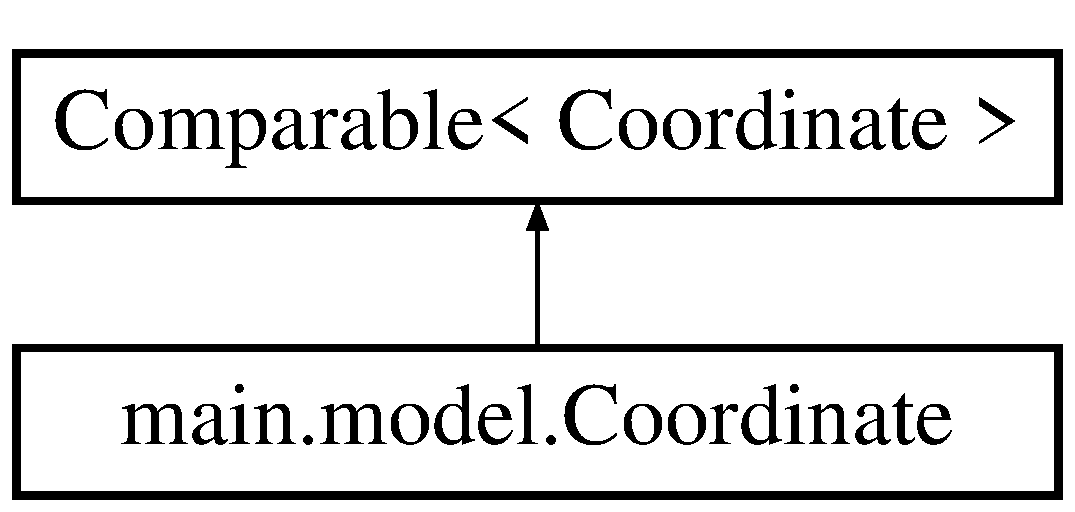
\includegraphics[height=2.000000cm]{classmain_1_1model_1_1_coordinate}
\end{center}
\end{figure}
\subsection*{Public Member Functions}
\begin{DoxyCompactItemize}
\item 
\hyperlink{classmain_1_1model_1_1_coordinate_adf838f26901635ae28525143e21c1263}{Coordinate} (int x, int y)
\item 
String \hyperlink{classmain_1_1model_1_1_coordinate_abf2f4212b8c3dd47c5cbc735935733f3}{to\+String} ()
\item 
boolean \hyperlink{classmain_1_1model_1_1_coordinate_a1e984b946ab806ab6921358700dc4619}{equals} (Object other)
\item 
int \hyperlink{classmain_1_1model_1_1_coordinate_ae3d33c4d690428f5daadea5380cf801a}{compare\+To} (\hyperlink{classmain_1_1model_1_1_coordinate}{Coordinate} coord)
\end{DoxyCompactItemize}
\subsection*{Static Public Member Functions}
\begin{DoxyCompactItemize}
\item 
static boolean \hyperlink{classmain_1_1model_1_1_coordinate_a438e61b11e63eb9522f754e84ecbee40}{valid\+Coordinate} (int x, int y)
\end{DoxyCompactItemize}
\subsection*{Public Attributes}
\begin{DoxyCompactItemize}
\item 
\hypertarget{classmain_1_1model_1_1_coordinate_a37010d49275f09df78e0f5d8ffefea31}{}\label{classmain_1_1model_1_1_coordinate_a37010d49275f09df78e0f5d8ffefea31} 
int {\bfseries x}
\item 
\hypertarget{classmain_1_1model_1_1_coordinate_a41308ad939f7cba09484c17abef5ea62}{}\label{classmain_1_1model_1_1_coordinate_a41308ad939f7cba09484c17abef5ea62} 
int {\bfseries y}
\end{DoxyCompactItemize}


\subsection{Detailed Description}
Created by samir on 9/1/16. 

\subsection{Constructor \& Destructor Documentation}
\hypertarget{classmain_1_1model_1_1_coordinate_adf838f26901635ae28525143e21c1263}{}\label{classmain_1_1model_1_1_coordinate_adf838f26901635ae28525143e21c1263} 
\index{main\+::model\+::\+Coordinate@{main\+::model\+::\+Coordinate}!Coordinate@{Coordinate}}
\index{Coordinate@{Coordinate}!main\+::model\+::\+Coordinate@{main\+::model\+::\+Coordinate}}
\subsubsection{\texorpdfstring{Coordinate()}{Coordinate()}}
{\footnotesize\ttfamily main.\+model.\+Coordinate.\+Coordinate (\begin{DoxyParamCaption}\item[{int}]{x,  }\item[{int}]{y }\end{DoxyParamCaption})}

Constructor taking in an x and y coordinate 

\subsection{Member Function Documentation}
\hypertarget{classmain_1_1model_1_1_coordinate_ae3d33c4d690428f5daadea5380cf801a}{}\label{classmain_1_1model_1_1_coordinate_ae3d33c4d690428f5daadea5380cf801a} 
\index{main\+::model\+::\+Coordinate@{main\+::model\+::\+Coordinate}!compare\+To@{compare\+To}}
\index{compare\+To@{compare\+To}!main\+::model\+::\+Coordinate@{main\+::model\+::\+Coordinate}}
\subsubsection{\texorpdfstring{compare\+To()}{compareTo()}}
{\footnotesize\ttfamily int main.\+model.\+Coordinate.\+compare\+To (\begin{DoxyParamCaption}\item[{\hyperlink{classmain_1_1model_1_1_coordinate}{Coordinate}}]{coord }\end{DoxyParamCaption})}

Comparator for Coordinates to allow for consistent sorting of arrays \hypertarget{classmain_1_1model_1_1_coordinate_a1e984b946ab806ab6921358700dc4619}{}\label{classmain_1_1model_1_1_coordinate_a1e984b946ab806ab6921358700dc4619} 
\index{main\+::model\+::\+Coordinate@{main\+::model\+::\+Coordinate}!equals@{equals}}
\index{equals@{equals}!main\+::model\+::\+Coordinate@{main\+::model\+::\+Coordinate}}
\subsubsection{\texorpdfstring{equals()}{equals()}}
{\footnotesize\ttfamily boolean main.\+model.\+Coordinate.\+equals (\begin{DoxyParamCaption}\item[{Object}]{other }\end{DoxyParamCaption})}

Equality operator for Coordinates (equal x and y values) \hypertarget{classmain_1_1model_1_1_coordinate_abf2f4212b8c3dd47c5cbc735935733f3}{}\label{classmain_1_1model_1_1_coordinate_abf2f4212b8c3dd47c5cbc735935733f3} 
\index{main\+::model\+::\+Coordinate@{main\+::model\+::\+Coordinate}!to\+String@{to\+String}}
\index{to\+String@{to\+String}!main\+::model\+::\+Coordinate@{main\+::model\+::\+Coordinate}}
\subsubsection{\texorpdfstring{to\+String()}{toString()}}
{\footnotesize\ttfamily String main.\+model.\+Coordinate.\+to\+String (\begin{DoxyParamCaption}{ }\end{DoxyParamCaption})}

String representation of a \hyperlink{classmain_1_1model_1_1_coordinate}{Coordinate} \hypertarget{classmain_1_1model_1_1_coordinate_a438e61b11e63eb9522f754e84ecbee40}{}\label{classmain_1_1model_1_1_coordinate_a438e61b11e63eb9522f754e84ecbee40} 
\index{main\+::model\+::\+Coordinate@{main\+::model\+::\+Coordinate}!valid\+Coordinate@{valid\+Coordinate}}
\index{valid\+Coordinate@{valid\+Coordinate}!main\+::model\+::\+Coordinate@{main\+::model\+::\+Coordinate}}
\subsubsection{\texorpdfstring{valid\+Coordinate()}{validCoordinate()}}
{\footnotesize\ttfamily static boolean main.\+model.\+Coordinate.\+valid\+Coordinate (\begin{DoxyParamCaption}\item[{int}]{x,  }\item[{int}]{y }\end{DoxyParamCaption})\hspace{0.3cm}{\ttfamily [static]}}

Check if the x and y values are legitimate coordinates 

The documentation for this class was generated from the following file\+:\begin{DoxyCompactItemize}
\item 
src/main/model/Coordinate.\+java\end{DoxyCompactItemize}

\hypertarget{classmain_1_1pieces_1_1_ferz}{}\section{main.\+pieces.\+Ferz Class Reference}
\label{classmain_1_1pieces_1_1_ferz}\index{main.\+pieces.\+Ferz@{main.\+pieces.\+Ferz}}
Inheritance diagram for main.\+pieces.\+Ferz\+:\begin{figure}[H]
\begin{center}
\leavevmode
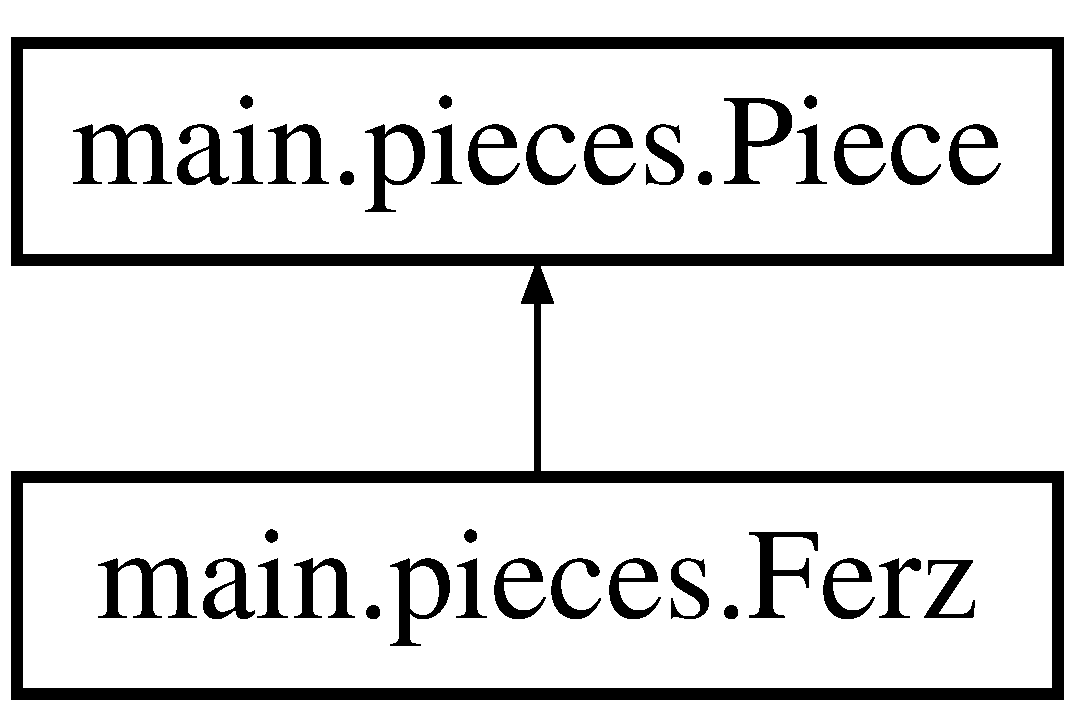
\includegraphics[height=2.000000cm]{classmain_1_1pieces_1_1_ferz}
\end{center}
\end{figure}
\subsection*{Public Member Functions}
\begin{DoxyCompactItemize}
\item 
\hyperlink{classmain_1_1pieces_1_1_ferz_a84fcf93b3400ec63737f39bd30f0083c}{Ferz} (String color)
\item 
String \hyperlink{classmain_1_1pieces_1_1_ferz_ad103c7f8a3d02e36fb8d6a52db0ef7cc}{get\+Type} ()
\item 
String \hyperlink{classmain_1_1pieces_1_1_ferz_ad4b187dafd0c861a6dbb0874e4245b79}{to\+String} ()
\item 
Array\+List$<$ \hyperlink{classmain_1_1model_1_1_coordinate}{Coordinate} $>$ \hyperlink{classmain_1_1pieces_1_1_ferz_a46bd9fd8889a0209540603f723b233af}{possible\+Moves} ()
\end{DoxyCompactItemize}
\subsection*{Additional Inherited Members}


\subsection{Detailed Description}
Created by samir on 9/13/16.

A custom piece that moves like a bishop but can only go one square 

\subsection{Constructor \& Destructor Documentation}
\hypertarget{classmain_1_1pieces_1_1_ferz_a84fcf93b3400ec63737f39bd30f0083c}{}\label{classmain_1_1pieces_1_1_ferz_a84fcf93b3400ec63737f39bd30f0083c} 
\index{main\+::pieces\+::\+Ferz@{main\+::pieces\+::\+Ferz}!Ferz@{Ferz}}
\index{Ferz@{Ferz}!main\+::pieces\+::\+Ferz@{main\+::pieces\+::\+Ferz}}
\subsubsection{\texorpdfstring{Ferz()}{Ferz()}}
{\footnotesize\ttfamily main.\+pieces.\+Ferz.\+Ferz (\begin{DoxyParamCaption}\item[{String}]{color }\end{DoxyParamCaption})}

\hyperlink{classmain_1_1pieces_1_1_ferz}{Ferz} constructor 
\begin{DoxyParams}{Parameters}
{\em color} & \\
\hline
\end{DoxyParams}


\subsection{Member Function Documentation}
\hypertarget{classmain_1_1pieces_1_1_ferz_ad103c7f8a3d02e36fb8d6a52db0ef7cc}{}\label{classmain_1_1pieces_1_1_ferz_ad103c7f8a3d02e36fb8d6a52db0ef7cc} 
\index{main\+::pieces\+::\+Ferz@{main\+::pieces\+::\+Ferz}!get\+Type@{get\+Type}}
\index{get\+Type@{get\+Type}!main\+::pieces\+::\+Ferz@{main\+::pieces\+::\+Ferz}}
\subsubsection{\texorpdfstring{get\+Type()}{getType()}}
{\footnotesize\ttfamily String main.\+pieces.\+Ferz.\+get\+Type (\begin{DoxyParamCaption}{ }\end{DoxyParamCaption})}

Return the type of piece \begin{DoxyReturn}{Returns}

\end{DoxyReturn}
\hypertarget{classmain_1_1pieces_1_1_ferz_a46bd9fd8889a0209540603f723b233af}{}\label{classmain_1_1pieces_1_1_ferz_a46bd9fd8889a0209540603f723b233af} 
\index{main\+::pieces\+::\+Ferz@{main\+::pieces\+::\+Ferz}!possible\+Moves@{possible\+Moves}}
\index{possible\+Moves@{possible\+Moves}!main\+::pieces\+::\+Ferz@{main\+::pieces\+::\+Ferz}}
\subsubsection{\texorpdfstring{possible\+Moves()}{possibleMoves()}}
{\footnotesize\ttfamily Array\+List$<$\hyperlink{classmain_1_1model_1_1_coordinate}{Coordinate}$>$ main.\+pieces.\+Ferz.\+possible\+Moves (\begin{DoxyParamCaption}{ }\end{DoxyParamCaption})}

Return an Array\+List of Coordinates of possible moves the \hyperlink{classmain_1_1pieces_1_1_ferz}{Ferz} can make \begin{DoxyReturn}{Returns}

\end{DoxyReturn}
\hypertarget{classmain_1_1pieces_1_1_ferz_ad4b187dafd0c861a6dbb0874e4245b79}{}\label{classmain_1_1pieces_1_1_ferz_ad4b187dafd0c861a6dbb0874e4245b79} 
\index{main\+::pieces\+::\+Ferz@{main\+::pieces\+::\+Ferz}!to\+String@{to\+String}}
\index{to\+String@{to\+String}!main\+::pieces\+::\+Ferz@{main\+::pieces\+::\+Ferz}}
\subsubsection{\texorpdfstring{to\+String()}{toString()}}
{\footnotesize\ttfamily String main.\+pieces.\+Ferz.\+to\+String (\begin{DoxyParamCaption}{ }\end{DoxyParamCaption})}

String representation of a \hyperlink{classmain_1_1pieces_1_1_ferz}{Ferz} \begin{DoxyReturn}{Returns}

\end{DoxyReturn}


The documentation for this class was generated from the following file\+:\begin{DoxyCompactItemize}
\item 
src/main/pieces/Ferz.\+java\end{DoxyCompactItemize}

\hypertarget{classtests_1_1pieces_1_1_ferz_test}{}\section{tests.\+pieces.\+Ferz\+Test Class Reference}
\label{classtests_1_1pieces_1_1_ferz_test}\index{tests.\+pieces.\+Ferz\+Test@{tests.\+pieces.\+Ferz\+Test}}
\subsection*{Public Member Functions}
\begin{DoxyCompactItemize}
\item 
\hypertarget{classtests_1_1pieces_1_1_ferz_test_a749f621df6526170fce1b73027f37e24}{}\label{classtests_1_1pieces_1_1_ferz_test_a749f621df6526170fce1b73027f37e24} 
void {\bfseries valid\+Ferz\+Constructor} ()  throws Exception 
\item 
\hypertarget{classtests_1_1pieces_1_1_ferz_test_abef0326a5f5a18b5a3222960db123796}{}\label{classtests_1_1pieces_1_1_ferz_test_abef0326a5f5a18b5a3222960db123796} 
void {\bfseries valid\+Ferz\+Movement} ()  throws Exception 
\item 
\hypertarget{classtests_1_1pieces_1_1_ferz_test_acb84f9a4456bcf2d2a37de394513dd66}{}\label{classtests_1_1pieces_1_1_ferz_test_acb84f9a4456bcf2d2a37de394513dd66} 
void {\bfseries invalid\+Ferz\+Movement} ()  throws Exception 
\end{DoxyCompactItemize}


\subsection{Detailed Description}
Created by samir on 9/13/16. 

The documentation for this class was generated from the following file\+:\begin{DoxyCompactItemize}
\item 
src/tests/pieces/Ferz\+Test.\+java\end{DoxyCompactItemize}

\hypertarget{classmain_1_1_game_controller}{}\section{main.\+Game\+Controller Class Reference}
\label{classmain_1_1_game_controller}\index{main.\+Game\+Controller@{main.\+Game\+Controller}}
\subsection*{Public Member Functions}
\begin{DoxyCompactItemize}
\item 
\hyperlink{classmain_1_1_game_controller_a455fa762af5d53a326a0c586fe4dcfe4}{Game\+Controller} ()
\item 
String \hyperlink{classmain_1_1_game_controller_acd8e5da713b1029f841ddd7fe9b54d0d}{get\+Current\+Move\+Color} ()
\item 
void \hyperlink{classmain_1_1_game_controller_a988e49925efe78aff8e776af38964b7b}{run\+Game} ()
\item 
void \hyperlink{classmain_1_1_game_controller_aa8c33e3c78ef79c96207ee507fe4f29b}{reset\+Game\+State} ()
\item 
void \hyperlink{classmain_1_1_game_controller_a810118fdb7712c718031ecc6464f3123}{reset\+Current\+Move\+State} ()
\item 
void \hyperlink{classmain_1_1_game_controller_a46df83552d6ea7c824e3eb13dc95d6c4}{piece\+Square\+Click} (int x, int y)
\item 
void \hyperlink{classmain_1_1_game_controller_a469b3da25d6a5ee02984379328262965}{empty\+Square\+Click} (int x, int y)
\item 
\hypertarget{classmain_1_1_game_controller_a88954a71a73f53a1c0be604dc99d235f}{}\label{classmain_1_1_game_controller_a88954a71a73f53a1c0be604dc99d235f} 
void {\bfseries handle\+Game\+Start} ()
\item 
void \hyperlink{classmain_1_1_game_controller_ac965ec2ce1c31547f9d219acca840629}{handle\+Game\+Undo} ()
\item 
void \hyperlink{classmain_1_1_game_controller_a328600841ad583141ff90225ef520d82}{handle\+Game\+Restart} ()
\item 
void \hyperlink{classmain_1_1_game_controller_a864236ccf74601951d818826253123d4}{handle\+Game\+Forfeit} ()
\item 
void \hyperlink{classmain_1_1_game_controller_a8291acf4ec3e1dc1cabdcb2a23c70e16}{handle\+Game\+Quit} ()
\item 
void \hyperlink{classmain_1_1_game_controller_ae75c41f7d73fe335be348d54a8e8c4e6}{handle\+Game\+Custom} ()
\end{DoxyCompactItemize}
\subsection*{Static Public Member Functions}
\begin{DoxyCompactItemize}
\item 
static void \hyperlink{classmain_1_1_game_controller_a92e6cb717e1d095d52e1f3db9899b3b4}{sleep} (int ms)
\item 
static void \hyperlink{classmain_1_1_game_controller_a868da5d6ac8b5b1d1c90cfb3957e2c3d}{main} (String\mbox{[}$\,$\mbox{]} args)
\end{DoxyCompactItemize}
\subsection*{Static Public Attributes}
\begin{DoxyCompactItemize}
\item 
\hypertarget{classmain_1_1_game_controller_a7aecbb578b9ec77925dd8a5fbd1c3841}{}\label{classmain_1_1_game_controller_a7aecbb578b9ec77925dd8a5fbd1c3841} 
static int {\bfseries length} = 8
\item 
\hypertarget{classmain_1_1_game_controller_a7b79e272fdf025df06ef83134c5f00f5}{}\label{classmain_1_1_game_controller_a7b79e272fdf025df06ef83134c5f00f5} 
static int {\bfseries width} = 8
\end{DoxyCompactItemize}
\subsection*{Protected Attributes}
\begin{DoxyCompactItemize}
\item 
\hypertarget{classmain_1_1_game_controller_a8a1459a02deb30c69520506ca6d52e4d}{}\label{classmain_1_1_game_controller_a8a1459a02deb30c69520506ca6d52e4d} 
\hyperlink{classmain_1_1model_1_1_coordinate}{Coordinate} {\bfseries start\+Coordinate} = null
\end{DoxyCompactItemize}


\subsection{Constructor \& Destructor Documentation}
\hypertarget{classmain_1_1_game_controller_a455fa762af5d53a326a0c586fe4dcfe4}{}\label{classmain_1_1_game_controller_a455fa762af5d53a326a0c586fe4dcfe4} 
\index{main\+::\+Game\+Controller@{main\+::\+Game\+Controller}!Game\+Controller@{Game\+Controller}}
\index{Game\+Controller@{Game\+Controller}!main\+::\+Game\+Controller@{main\+::\+Game\+Controller}}
\subsubsection{\texorpdfstring{Game\+Controller()}{GameController()}}
{\footnotesize\ttfamily main.\+Game\+Controller.\+Game\+Controller (\begin{DoxyParamCaption}{ }\end{DoxyParamCaption})}

\hyperlink{classmain_1_1_game_controller}{Game\+Controller} constructor which runs the game 

\subsection{Member Function Documentation}
\hypertarget{classmain_1_1_game_controller_a469b3da25d6a5ee02984379328262965}{}\label{classmain_1_1_game_controller_a469b3da25d6a5ee02984379328262965} 
\index{main\+::\+Game\+Controller@{main\+::\+Game\+Controller}!empty\+Square\+Click@{empty\+Square\+Click}}
\index{empty\+Square\+Click@{empty\+Square\+Click}!main\+::\+Game\+Controller@{main\+::\+Game\+Controller}}
\subsubsection{\texorpdfstring{empty\+Square\+Click()}{emptySquareClick()}}
{\footnotesize\ttfamily void main.\+Game\+Controller.\+empty\+Square\+Click (\begin{DoxyParamCaption}\item[{int}]{x,  }\item[{int}]{y }\end{DoxyParamCaption})}

Action to take when an empty square is clicked If a piece has already been selected, check if the clicked square is in the set of possible moves for the piece. If it is, try making the move to see if it puts the player in check. If not, alert the player of the invalid move 
\begin{DoxyParams}{Parameters}
{\em x} & \\
\hline
{\em y} & \\
\hline
\end{DoxyParams}
\hypertarget{classmain_1_1_game_controller_acd8e5da713b1029f841ddd7fe9b54d0d}{}\label{classmain_1_1_game_controller_acd8e5da713b1029f841ddd7fe9b54d0d} 
\index{main\+::\+Game\+Controller@{main\+::\+Game\+Controller}!get\+Current\+Move\+Color@{get\+Current\+Move\+Color}}
\index{get\+Current\+Move\+Color@{get\+Current\+Move\+Color}!main\+::\+Game\+Controller@{main\+::\+Game\+Controller}}
\subsubsection{\texorpdfstring{get\+Current\+Move\+Color()}{getCurrentMoveColor()}}
{\footnotesize\ttfamily String main.\+Game\+Controller.\+get\+Current\+Move\+Color (\begin{DoxyParamCaption}{ }\end{DoxyParamCaption})}

Return the current move color \begin{DoxyReturn}{Returns}

\end{DoxyReturn}
\hypertarget{classmain_1_1_game_controller_ae75c41f7d73fe335be348d54a8e8c4e6}{}\label{classmain_1_1_game_controller_ae75c41f7d73fe335be348d54a8e8c4e6} 
\index{main\+::\+Game\+Controller@{main\+::\+Game\+Controller}!handle\+Game\+Custom@{handle\+Game\+Custom}}
\index{handle\+Game\+Custom@{handle\+Game\+Custom}!main\+::\+Game\+Controller@{main\+::\+Game\+Controller}}
\subsubsection{\texorpdfstring{handle\+Game\+Custom()}{handleGameCustom()}}
{\footnotesize\ttfamily void main.\+Game\+Controller.\+handle\+Game\+Custom (\begin{DoxyParamCaption}{ }\end{DoxyParamCaption})}

Add the custom pieces to the model Can only be used when the game has not started yet \hypertarget{classmain_1_1_game_controller_a864236ccf74601951d818826253123d4}{}\label{classmain_1_1_game_controller_a864236ccf74601951d818826253123d4} 
\index{main\+::\+Game\+Controller@{main\+::\+Game\+Controller}!handle\+Game\+Forfeit@{handle\+Game\+Forfeit}}
\index{handle\+Game\+Forfeit@{handle\+Game\+Forfeit}!main\+::\+Game\+Controller@{main\+::\+Game\+Controller}}
\subsubsection{\texorpdfstring{handle\+Game\+Forfeit()}{handleGameForfeit()}}
{\footnotesize\ttfamily void main.\+Game\+Controller.\+handle\+Game\+Forfeit (\begin{DoxyParamCaption}{ }\end{DoxyParamCaption})}

If the game is forfeited, end the current game Mark the other player as the winner of this game \hypertarget{classmain_1_1_game_controller_a8291acf4ec3e1dc1cabdcb2a23c70e16}{}\label{classmain_1_1_game_controller_a8291acf4ec3e1dc1cabdcb2a23c70e16} 
\index{main\+::\+Game\+Controller@{main\+::\+Game\+Controller}!handle\+Game\+Quit@{handle\+Game\+Quit}}
\index{handle\+Game\+Quit@{handle\+Game\+Quit}!main\+::\+Game\+Controller@{main\+::\+Game\+Controller}}
\subsubsection{\texorpdfstring{handle\+Game\+Quit()}{handleGameQuit()}}
{\footnotesize\ttfamily void main.\+Game\+Controller.\+handle\+Game\+Quit (\begin{DoxyParamCaption}{ }\end{DoxyParamCaption})}

If the game is quit, exit the game. \hypertarget{classmain_1_1_game_controller_a328600841ad583141ff90225ef520d82}{}\label{classmain_1_1_game_controller_a328600841ad583141ff90225ef520d82} 
\index{main\+::\+Game\+Controller@{main\+::\+Game\+Controller}!handle\+Game\+Restart@{handle\+Game\+Restart}}
\index{handle\+Game\+Restart@{handle\+Game\+Restart}!main\+::\+Game\+Controller@{main\+::\+Game\+Controller}}
\subsubsection{\texorpdfstring{handle\+Game\+Restart()}{handleGameRestart()}}
{\footnotesize\ttfamily void main.\+Game\+Controller.\+handle\+Game\+Restart (\begin{DoxyParamCaption}{ }\end{DoxyParamCaption})}

If the restart button is pressed, pop up a confirmation If no or window closed, ignore. If yes, notify the players, stop the current game, and reset the G\+UI state \hypertarget{classmain_1_1_game_controller_ac965ec2ce1c31547f9d219acca840629}{}\label{classmain_1_1_game_controller_ac965ec2ce1c31547f9d219acca840629} 
\index{main\+::\+Game\+Controller@{main\+::\+Game\+Controller}!handle\+Game\+Undo@{handle\+Game\+Undo}}
\index{handle\+Game\+Undo@{handle\+Game\+Undo}!main\+::\+Game\+Controller@{main\+::\+Game\+Controller}}
\subsubsection{\texorpdfstring{handle\+Game\+Undo()}{handleGameUndo()}}
{\footnotesize\ttfamily void main.\+Game\+Controller.\+handle\+Game\+Undo (\begin{DoxyParamCaption}{ }\end{DoxyParamCaption})}

Undo the move if last\+Move is not null (i.\+e. move has been made or move not already undone). If undoing the move, switch turns back to the original player\textquotesingle{}s move Else, alert the player that an undo is not valid \hypertarget{classmain_1_1_game_controller_a868da5d6ac8b5b1d1c90cfb3957e2c3d}{}\label{classmain_1_1_game_controller_a868da5d6ac8b5b1d1c90cfb3957e2c3d} 
\index{main\+::\+Game\+Controller@{main\+::\+Game\+Controller}!main@{main}}
\index{main@{main}!main\+::\+Game\+Controller@{main\+::\+Game\+Controller}}
\subsubsection{\texorpdfstring{main()}{main()}}
{\footnotesize\ttfamily static void main.\+Game\+Controller.\+main (\begin{DoxyParamCaption}\item[{String \mbox{[}$\,$\mbox{]}}]{args }\end{DoxyParamCaption})\hspace{0.3cm}{\ttfamily [static]}}

Create a new game 
\begin{DoxyParams}{Parameters}
{\em args} & \\
\hline
\end{DoxyParams}
\hypertarget{classmain_1_1_game_controller_a46df83552d6ea7c824e3eb13dc95d6c4}{}\label{classmain_1_1_game_controller_a46df83552d6ea7c824e3eb13dc95d6c4} 
\index{main\+::\+Game\+Controller@{main\+::\+Game\+Controller}!piece\+Square\+Click@{piece\+Square\+Click}}
\index{piece\+Square\+Click@{piece\+Square\+Click}!main\+::\+Game\+Controller@{main\+::\+Game\+Controller}}
\subsubsection{\texorpdfstring{piece\+Square\+Click()}{pieceSquareClick()}}
{\footnotesize\ttfamily void main.\+Game\+Controller.\+piece\+Square\+Click (\begin{DoxyParamCaption}\item[{int}]{x,  }\item[{int}]{y }\end{DoxyParamCaption})}

Action to take when a piece square is clicked If no piece has already been selected, select this piece if a valid piece 
\begin{DoxyParams}{Parameters}
{\em x} & \\
\hline
{\em y} & \\
\hline
\end{DoxyParams}
\hypertarget{classmain_1_1_game_controller_a810118fdb7712c718031ecc6464f3123}{}\label{classmain_1_1_game_controller_a810118fdb7712c718031ecc6464f3123} 
\index{main\+::\+Game\+Controller@{main\+::\+Game\+Controller}!reset\+Current\+Move\+State@{reset\+Current\+Move\+State}}
\index{reset\+Current\+Move\+State@{reset\+Current\+Move\+State}!main\+::\+Game\+Controller@{main\+::\+Game\+Controller}}
\subsubsection{\texorpdfstring{reset\+Current\+Move\+State()}{resetCurrentMoveState()}}
{\footnotesize\ttfamily void main.\+Game\+Controller.\+reset\+Current\+Move\+State (\begin{DoxyParamCaption}{ }\end{DoxyParamCaption})}

Reset the G\+UI state and highlights \hypertarget{classmain_1_1_game_controller_aa8c33e3c78ef79c96207ee507fe4f29b}{}\label{classmain_1_1_game_controller_aa8c33e3c78ef79c96207ee507fe4f29b} 
\index{main\+::\+Game\+Controller@{main\+::\+Game\+Controller}!reset\+Game\+State@{reset\+Game\+State}}
\index{reset\+Game\+State@{reset\+Game\+State}!main\+::\+Game\+Controller@{main\+::\+Game\+Controller}}
\subsubsection{\texorpdfstring{reset\+Game\+State()}{resetGameState()}}
{\footnotesize\ttfamily void main.\+Game\+Controller.\+reset\+Game\+State (\begin{DoxyParamCaption}{ }\end{DoxyParamCaption})}

Reset the game states of forfeit, restart, and quit \hypertarget{classmain_1_1_game_controller_a988e49925efe78aff8e776af38964b7b}{}\label{classmain_1_1_game_controller_a988e49925efe78aff8e776af38964b7b} 
\index{main\+::\+Game\+Controller@{main\+::\+Game\+Controller}!run\+Game@{run\+Game}}
\index{run\+Game@{run\+Game}!main\+::\+Game\+Controller@{main\+::\+Game\+Controller}}
\subsubsection{\texorpdfstring{run\+Game()}{runGame()}}
{\footnotesize\ttfamily void main.\+Game\+Controller.\+run\+Game (\begin{DoxyParamCaption}{ }\end{DoxyParamCaption})}

Keep looping to run the game until the current game is stopped \hypertarget{classmain_1_1_game_controller_a92e6cb717e1d095d52e1f3db9899b3b4}{}\label{classmain_1_1_game_controller_a92e6cb717e1d095d52e1f3db9899b3b4} 
\index{main\+::\+Game\+Controller@{main\+::\+Game\+Controller}!sleep@{sleep}}
\index{sleep@{sleep}!main\+::\+Game\+Controller@{main\+::\+Game\+Controller}}
\subsubsection{\texorpdfstring{sleep()}{sleep()}}
{\footnotesize\ttfamily static void main.\+Game\+Controller.\+sleep (\begin{DoxyParamCaption}\item[{int}]{ms }\end{DoxyParamCaption})\hspace{0.3cm}{\ttfamily [static]}}

Sleep a thread ms number of milliseconds Catch and print out any exceptions 
\begin{DoxyParams}{Parameters}
{\em ms} & \\
\hline
\end{DoxyParams}


The documentation for this class was generated from the following file\+:\begin{DoxyCompactItemize}
\item 
src/main/Game\+Controller.\+java\end{DoxyCompactItemize}

\hypertarget{classmain_1_1model_1_1_initializer}{}\section{main.\+model.\+Initializer Class Reference}
\label{classmain_1_1model_1_1_initializer}\index{main.\+model.\+Initializer@{main.\+model.\+Initializer}}
\subsection*{Static Public Member Functions}
\begin{DoxyCompactItemize}
\item 
static void \hyperlink{classmain_1_1model_1_1_initializer_a314022d0743a0169540f64e9b8b84988}{initialize\+Board} (\hyperlink{classmain_1_1model_1_1_board}{Board} board)
\end{DoxyCompactItemize}


\subsection{Detailed Description}
Created by samir on 9/12/16. 

\subsection{Member Function Documentation}
\hypertarget{classmain_1_1model_1_1_initializer_a314022d0743a0169540f64e9b8b84988}{}\label{classmain_1_1model_1_1_initializer_a314022d0743a0169540f64e9b8b84988} 
\index{main\+::model\+::\+Initializer@{main\+::model\+::\+Initializer}!initialize\+Board@{initialize\+Board}}
\index{initialize\+Board@{initialize\+Board}!main\+::model\+::\+Initializer@{main\+::model\+::\+Initializer}}
\subsubsection{\texorpdfstring{initialize\+Board()}{initializeBoard()}}
{\footnotesize\ttfamily static void main.\+model.\+Initializer.\+initialize\+Board (\begin{DoxyParamCaption}\item[{\hyperlink{classmain_1_1model_1_1_board}{Board}}]{board }\end{DoxyParamCaption})\hspace{0.3cm}{\ttfamily [static]}}

\subparagraph*{}

Initialization Methods \subparagraph*{}

The documentation for this class was generated from the following file\+:\begin{DoxyCompactItemize}
\item 
src/main/model/Initializer.\+java\end{DoxyCompactItemize}

\hypertarget{classmain_1_1pieces_1_1_king}{}\section{main.\+pieces.\+King Class Reference}
\label{classmain_1_1pieces_1_1_king}\index{main.\+pieces.\+King@{main.\+pieces.\+King}}
Inheritance diagram for main.\+pieces.\+King\+:\begin{figure}[H]
\begin{center}
\leavevmode
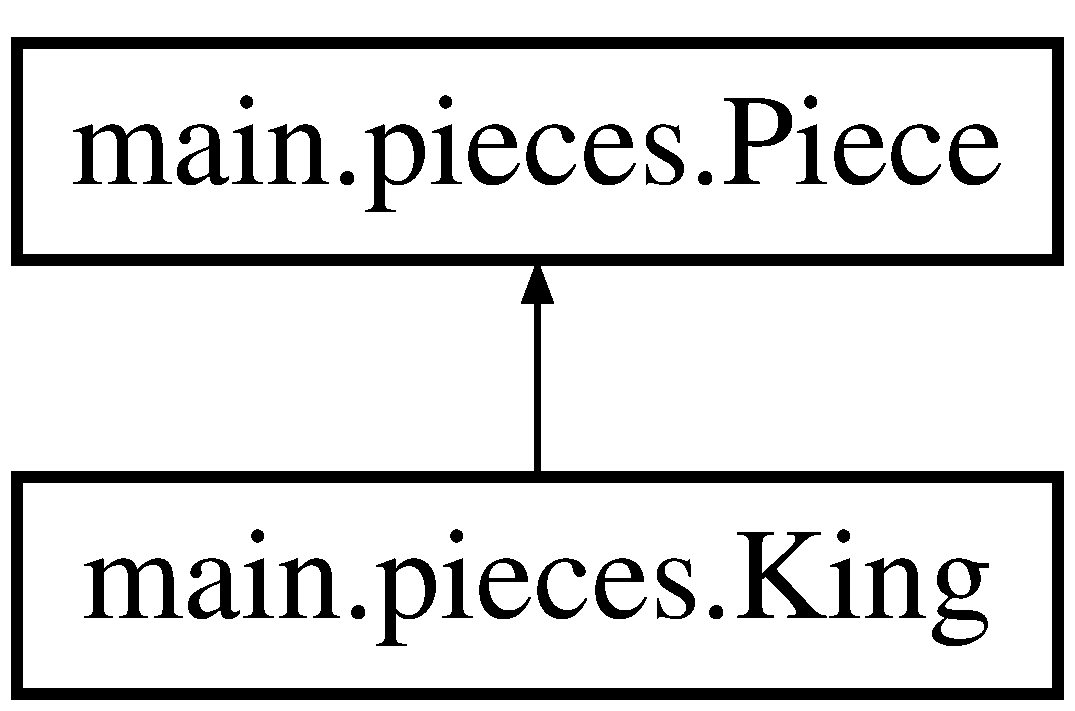
\includegraphics[height=2.000000cm]{classmain_1_1pieces_1_1_king}
\end{center}
\end{figure}
\subsection*{Public Member Functions}
\begin{DoxyCompactItemize}
\item 
\hyperlink{classmain_1_1pieces_1_1_king_aa8a03c9941ca3522dea1a964f1ae15cf}{King} (String color)
\item 
String \hyperlink{classmain_1_1pieces_1_1_king_a357799158a941db860a25da4d0b9ec5a}{get\+Type} ()
\item 
String \hyperlink{classmain_1_1pieces_1_1_king_aa93a1ae4998482975674eeca33112961}{to\+String} ()
\item 
Array\+List$<$ \hyperlink{classmain_1_1model_1_1_coordinate}{Coordinate} $>$ \hyperlink{classmain_1_1pieces_1_1_king_afde71e97df359b784be2db1a66ac36b1}{possible\+Moves} ()
\end{DoxyCompactItemize}
\subsection*{Additional Inherited Members}


\subsection{Detailed Description}
Created by samir on 9/2/16. 

\subsection{Constructor \& Destructor Documentation}
\hypertarget{classmain_1_1pieces_1_1_king_aa8a03c9941ca3522dea1a964f1ae15cf}{}\label{classmain_1_1pieces_1_1_king_aa8a03c9941ca3522dea1a964f1ae15cf} 
\index{main\+::pieces\+::\+King@{main\+::pieces\+::\+King}!King@{King}}
\index{King@{King}!main\+::pieces\+::\+King@{main\+::pieces\+::\+King}}
\subsubsection{\texorpdfstring{King()}{King()}}
{\footnotesize\ttfamily main.\+pieces.\+King.\+King (\begin{DoxyParamCaption}\item[{String}]{color }\end{DoxyParamCaption})}

Constructor taking in an x and y coordinate 

\subsection{Member Function Documentation}
\hypertarget{classmain_1_1pieces_1_1_king_a357799158a941db860a25da4d0b9ec5a}{}\label{classmain_1_1pieces_1_1_king_a357799158a941db860a25da4d0b9ec5a} 
\index{main\+::pieces\+::\+King@{main\+::pieces\+::\+King}!get\+Type@{get\+Type}}
\index{get\+Type@{get\+Type}!main\+::pieces\+::\+King@{main\+::pieces\+::\+King}}
\subsubsection{\texorpdfstring{get\+Type()}{getType()}}
{\footnotesize\ttfamily String main.\+pieces.\+King.\+get\+Type (\begin{DoxyParamCaption}{ }\end{DoxyParamCaption})}

Returns the type of this piece \hypertarget{classmain_1_1pieces_1_1_king_afde71e97df359b784be2db1a66ac36b1}{}\label{classmain_1_1pieces_1_1_king_afde71e97df359b784be2db1a66ac36b1} 
\index{main\+::pieces\+::\+King@{main\+::pieces\+::\+King}!possible\+Moves@{possible\+Moves}}
\index{possible\+Moves@{possible\+Moves}!main\+::pieces\+::\+King@{main\+::pieces\+::\+King}}
\subsubsection{\texorpdfstring{possible\+Moves()}{possibleMoves()}}
{\footnotesize\ttfamily Array\+List$<$\hyperlink{classmain_1_1model_1_1_coordinate}{Coordinate}$>$ main.\+pieces.\+King.\+possible\+Moves (\begin{DoxyParamCaption}{ }\end{DoxyParamCaption})}

Returns an Array\+List with the coordinates of the possible moves that this king can make \hypertarget{classmain_1_1pieces_1_1_king_aa93a1ae4998482975674eeca33112961}{}\label{classmain_1_1pieces_1_1_king_aa93a1ae4998482975674eeca33112961} 
\index{main\+::pieces\+::\+King@{main\+::pieces\+::\+King}!to\+String@{to\+String}}
\index{to\+String@{to\+String}!main\+::pieces\+::\+King@{main\+::pieces\+::\+King}}
\subsubsection{\texorpdfstring{to\+String()}{toString()}}
{\footnotesize\ttfamily String main.\+pieces.\+King.\+to\+String (\begin{DoxyParamCaption}{ }\end{DoxyParamCaption})}

String representation of a \hyperlink{classmain_1_1pieces_1_1_king}{King} 

The documentation for this class was generated from the following file\+:\begin{DoxyCompactItemize}
\item 
src/main/pieces/King.\+java\end{DoxyCompactItemize}

\hypertarget{classtests_1_1pieces_1_1_king_test}{}\section{tests.\+pieces.\+King\+Test Class Reference}
\label{classtests_1_1pieces_1_1_king_test}\index{tests.\+pieces.\+King\+Test@{tests.\+pieces.\+King\+Test}}
\subsection*{Public Member Functions}
\begin{DoxyCompactItemize}
\item 
void \hyperlink{classtests_1_1pieces_1_1_king_test_a1d202d75c158a39040fc84f7a5e42db7}{valid\+Queen\+Constructor} ()  throws Exception 
\item 
void \hyperlink{classtests_1_1pieces_1_1_king_test_a50ab715ea6df03436f548340ca2f9ab6}{valid\+King\+Movement} ()  throws Exception 
\end{DoxyCompactItemize}


\subsection{Detailed Description}
Created by samir on 9/5/16. 

\subsection{Member Function Documentation}
\hypertarget{classtests_1_1pieces_1_1_king_test_a50ab715ea6df03436f548340ca2f9ab6}{}\label{classtests_1_1pieces_1_1_king_test_a50ab715ea6df03436f548340ca2f9ab6} 
\index{tests\+::pieces\+::\+King\+Test@{tests\+::pieces\+::\+King\+Test}!valid\+King\+Movement@{valid\+King\+Movement}}
\index{valid\+King\+Movement@{valid\+King\+Movement}!tests\+::pieces\+::\+King\+Test@{tests\+::pieces\+::\+King\+Test}}
\subsubsection{\texorpdfstring{valid\+King\+Movement()}{validKingMovement()}}
{\footnotesize\ttfamily void tests.\+pieces.\+King\+Test.\+valid\+King\+Movement (\begin{DoxyParamCaption}{ }\end{DoxyParamCaption}) throws Exception}

Test for valid queen movement (should be able to move) Check the valid moves match up 
\begin{DoxyExceptions}{Exceptions}
{\em Exception} & \\
\hline
\end{DoxyExceptions}
\hypertarget{classtests_1_1pieces_1_1_king_test_a1d202d75c158a39040fc84f7a5e42db7}{}\label{classtests_1_1pieces_1_1_king_test_a1d202d75c158a39040fc84f7a5e42db7} 
\index{tests\+::pieces\+::\+King\+Test@{tests\+::pieces\+::\+King\+Test}!valid\+Queen\+Constructor@{valid\+Queen\+Constructor}}
\index{valid\+Queen\+Constructor@{valid\+Queen\+Constructor}!tests\+::pieces\+::\+King\+Test@{tests\+::pieces\+::\+King\+Test}}
\subsubsection{\texorpdfstring{valid\+Queen\+Constructor()}{validQueenConstructor()}}
{\footnotesize\ttfamily void tests.\+pieces.\+King\+Test.\+valid\+Queen\+Constructor (\begin{DoxyParamCaption}{ }\end{DoxyParamCaption}) throws Exception}

Valid constructor for a king should not throw an exception 

The documentation for this class was generated from the following file\+:\begin{DoxyCompactItemize}
\item 
src/tests/pieces/King\+Test.\+java\end{DoxyCompactItemize}

\hypertarget{classmain_1_1pieces_1_1_knight}{}\section{main.\+pieces.\+Knight Class Reference}
\label{classmain_1_1pieces_1_1_knight}\index{main.\+pieces.\+Knight@{main.\+pieces.\+Knight}}
Inheritance diagram for main.\+pieces.\+Knight\+:\begin{figure}[H]
\begin{center}
\leavevmode
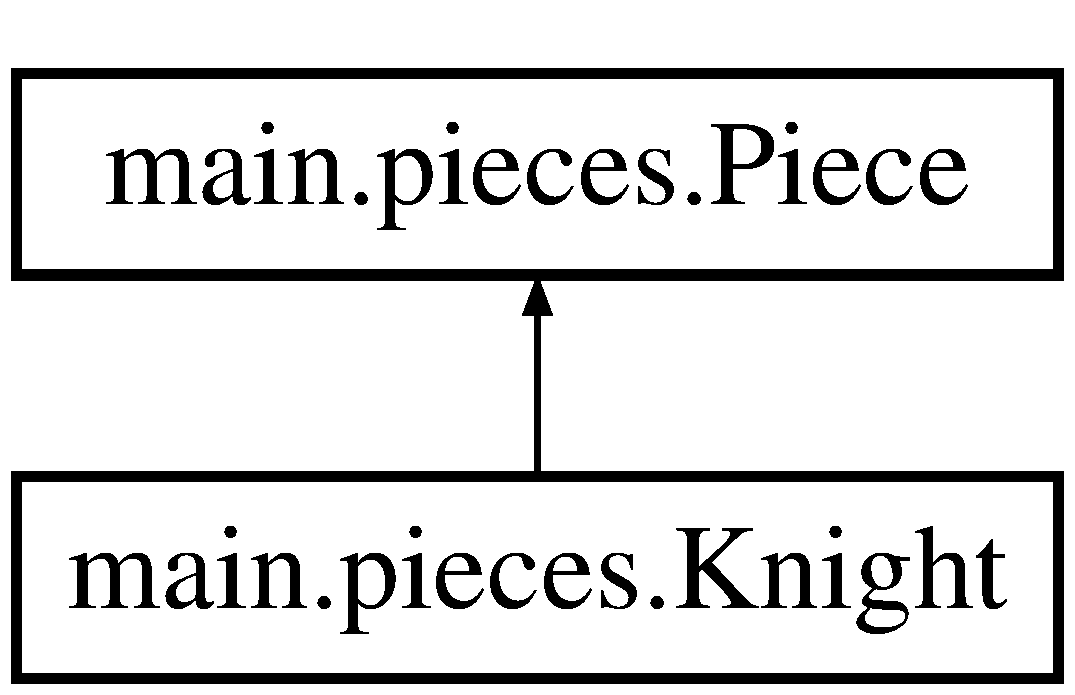
\includegraphics[height=2.000000cm]{classmain_1_1pieces_1_1_knight}
\end{center}
\end{figure}
\subsection*{Public Member Functions}
\begin{DoxyCompactItemize}
\item 
\hyperlink{classmain_1_1pieces_1_1_knight_a0db1e21cc4f2fa35655c2ee4ae00c9d5}{Knight} (String color)
\item 
String \hyperlink{classmain_1_1pieces_1_1_knight_a6c453a86bbecb2936ea4c7c472ebf360}{get\+Type} ()
\item 
String \hyperlink{classmain_1_1pieces_1_1_knight_aaf2e8a203e5875f9429eb528616adc53}{to\+String} ()
\item 
Array\+List$<$ \hyperlink{classmain_1_1model_1_1_coordinate}{Coordinate} $>$ \hyperlink{classmain_1_1pieces_1_1_knight_a9aa67ae101fd96efce020323b45511a7}{possible\+Moves} ()
\end{DoxyCompactItemize}
\subsection*{Additional Inherited Members}


\subsection{Detailed Description}
Created by samir on 9/2/16. 

\subsection{Constructor \& Destructor Documentation}
\hypertarget{classmain_1_1pieces_1_1_knight_a0db1e21cc4f2fa35655c2ee4ae00c9d5}{}\label{classmain_1_1pieces_1_1_knight_a0db1e21cc4f2fa35655c2ee4ae00c9d5} 
\index{main\+::pieces\+::\+Knight@{main\+::pieces\+::\+Knight}!Knight@{Knight}}
\index{Knight@{Knight}!main\+::pieces\+::\+Knight@{main\+::pieces\+::\+Knight}}
\subsubsection{\texorpdfstring{Knight()}{Knight()}}
{\footnotesize\ttfamily main.\+pieces.\+Knight.\+Knight (\begin{DoxyParamCaption}\item[{String}]{color }\end{DoxyParamCaption})}

Constructor taking in an x and y coordinate 

\subsection{Member Function Documentation}
\hypertarget{classmain_1_1pieces_1_1_knight_a6c453a86bbecb2936ea4c7c472ebf360}{}\label{classmain_1_1pieces_1_1_knight_a6c453a86bbecb2936ea4c7c472ebf360} 
\index{main\+::pieces\+::\+Knight@{main\+::pieces\+::\+Knight}!get\+Type@{get\+Type}}
\index{get\+Type@{get\+Type}!main\+::pieces\+::\+Knight@{main\+::pieces\+::\+Knight}}
\subsubsection{\texorpdfstring{get\+Type()}{getType()}}
{\footnotesize\ttfamily String main.\+pieces.\+Knight.\+get\+Type (\begin{DoxyParamCaption}{ }\end{DoxyParamCaption})}

Returns the type of this piece \hypertarget{classmain_1_1pieces_1_1_knight_a9aa67ae101fd96efce020323b45511a7}{}\label{classmain_1_1pieces_1_1_knight_a9aa67ae101fd96efce020323b45511a7} 
\index{main\+::pieces\+::\+Knight@{main\+::pieces\+::\+Knight}!possible\+Moves@{possible\+Moves}}
\index{possible\+Moves@{possible\+Moves}!main\+::pieces\+::\+Knight@{main\+::pieces\+::\+Knight}}
\subsubsection{\texorpdfstring{possible\+Moves()}{possibleMoves()}}
{\footnotesize\ttfamily Array\+List$<$\hyperlink{classmain_1_1model_1_1_coordinate}{Coordinate}$>$ main.\+pieces.\+Knight.\+possible\+Moves (\begin{DoxyParamCaption}{ }\end{DoxyParamCaption})}

Returns an Array\+List with the coordinates of the possible moves this knight can make \begin{DoxyReturn}{Returns}

\end{DoxyReturn}
\hypertarget{classmain_1_1pieces_1_1_knight_aaf2e8a203e5875f9429eb528616adc53}{}\label{classmain_1_1pieces_1_1_knight_aaf2e8a203e5875f9429eb528616adc53} 
\index{main\+::pieces\+::\+Knight@{main\+::pieces\+::\+Knight}!to\+String@{to\+String}}
\index{to\+String@{to\+String}!main\+::pieces\+::\+Knight@{main\+::pieces\+::\+Knight}}
\subsubsection{\texorpdfstring{to\+String()}{toString()}}
{\footnotesize\ttfamily String main.\+pieces.\+Knight.\+to\+String (\begin{DoxyParamCaption}{ }\end{DoxyParamCaption})}

String representation of a \hyperlink{classmain_1_1pieces_1_1_knight}{Knight} 

The documentation for this class was generated from the following file\+:\begin{DoxyCompactItemize}
\item 
src/main/pieces/Knight.\+java\end{DoxyCompactItemize}

\hypertarget{classtests_1_1pieces_1_1_knight_test}{}\section{tests.\+pieces.\+Knight\+Test Class Reference}
\label{classtests_1_1pieces_1_1_knight_test}\index{tests.\+pieces.\+Knight\+Test@{tests.\+pieces.\+Knight\+Test}}
\subsection*{Public Member Functions}
\begin{DoxyCompactItemize}
\item 
void \hyperlink{classtests_1_1pieces_1_1_knight_test_ac63e8a47040357e6f02594034d0ecb75}{valid\+Knight\+Constructor} ()  throws Exception 
\item 
void \hyperlink{classtests_1_1pieces_1_1_knight_test_a1f441301e64a3dd8330a3646fcb25c0b}{valid\+Knight\+Movement} ()  throws Exception 
\item 
void \hyperlink{classtests_1_1pieces_1_1_knight_test_a8ac79409a204de610658fccd8bbb08ec}{invalid\+Knight\+Movement} ()  throws Exception 
\end{DoxyCompactItemize}


\subsection{Detailed Description}
Created by samir on 9/5/16. 

\subsection{Member Function Documentation}
\hypertarget{classtests_1_1pieces_1_1_knight_test_a8ac79409a204de610658fccd8bbb08ec}{}\label{classtests_1_1pieces_1_1_knight_test_a8ac79409a204de610658fccd8bbb08ec} 
\index{tests\+::pieces\+::\+Knight\+Test@{tests\+::pieces\+::\+Knight\+Test}!invalid\+Knight\+Movement@{invalid\+Knight\+Movement}}
\index{invalid\+Knight\+Movement@{invalid\+Knight\+Movement}!tests\+::pieces\+::\+Knight\+Test@{tests\+::pieces\+::\+Knight\+Test}}
\subsubsection{\texorpdfstring{invalid\+Knight\+Movement()}{invalidKnightMovement()}}
{\footnotesize\ttfamily void tests.\+pieces.\+Knight\+Test.\+invalid\+Knight\+Movement (\begin{DoxyParamCaption}{ }\end{DoxyParamCaption}) throws Exception}

Test for invalid knight movement Moving off the board\+G\+UI should be rejected \hypertarget{classtests_1_1pieces_1_1_knight_test_ac63e8a47040357e6f02594034d0ecb75}{}\label{classtests_1_1pieces_1_1_knight_test_ac63e8a47040357e6f02594034d0ecb75} 
\index{tests\+::pieces\+::\+Knight\+Test@{tests\+::pieces\+::\+Knight\+Test}!valid\+Knight\+Constructor@{valid\+Knight\+Constructor}}
\index{valid\+Knight\+Constructor@{valid\+Knight\+Constructor}!tests\+::pieces\+::\+Knight\+Test@{tests\+::pieces\+::\+Knight\+Test}}
\subsubsection{\texorpdfstring{valid\+Knight\+Constructor()}{validKnightConstructor()}}
{\footnotesize\ttfamily void tests.\+pieces.\+Knight\+Test.\+valid\+Knight\+Constructor (\begin{DoxyParamCaption}{ }\end{DoxyParamCaption}) throws Exception}

Valid constructor for a knight should not throw an exception \hypertarget{classtests_1_1pieces_1_1_knight_test_a1f441301e64a3dd8330a3646fcb25c0b}{}\label{classtests_1_1pieces_1_1_knight_test_a1f441301e64a3dd8330a3646fcb25c0b} 
\index{tests\+::pieces\+::\+Knight\+Test@{tests\+::pieces\+::\+Knight\+Test}!valid\+Knight\+Movement@{valid\+Knight\+Movement}}
\index{valid\+Knight\+Movement@{valid\+Knight\+Movement}!tests\+::pieces\+::\+Knight\+Test@{tests\+::pieces\+::\+Knight\+Test}}
\subsubsection{\texorpdfstring{valid\+Knight\+Movement()}{validKnightMovement()}}
{\footnotesize\ttfamily void tests.\+pieces.\+Knight\+Test.\+valid\+Knight\+Movement (\begin{DoxyParamCaption}{ }\end{DoxyParamCaption}) throws Exception}

Test for valid knight movement (should be able to move) Check the valid moves match up 
\begin{DoxyExceptions}{Exceptions}
{\em Exception} & \\
\hline
\end{DoxyExceptions}


The documentation for this class was generated from the following file\+:\begin{DoxyCompactItemize}
\item 
src/tests/pieces/Knight\+Test.\+java\end{DoxyCompactItemize}

\hypertarget{classmain_1_1model_1_1_move}{}\section{main.\+model.\+Move Class Reference}
\label{classmain_1_1model_1_1_move}\index{main.\+model.\+Move@{main.\+model.\+Move}}
\subsection*{Public Member Functions}
\begin{DoxyCompactItemize}
\item 
\hypertarget{classmain_1_1model_1_1_move_ae58ed72f93d320e6ac77a3d41763cf3a}{}\label{classmain_1_1model_1_1_move_ae58ed72f93d320e6ac77a3d41763cf3a} 
{\bfseries Move} (\hyperlink{classmain_1_1pieces_1_1_piece}{Piece} piece, \hyperlink{classmain_1_1pieces_1_1_piece}{Piece} existing, \hyperlink{classmain_1_1model_1_1_coordinate}{Coordinate} start, \hyperlink{classmain_1_1model_1_1_coordinate}{Coordinate} destination)
\end{DoxyCompactItemize}
\subsection*{Public Attributes}
\begin{DoxyCompactItemize}
\item 
\hypertarget{classmain_1_1model_1_1_move_ae178b74847fe536dad796f48390ae54c}{}\label{classmain_1_1model_1_1_move_ae178b74847fe536dad796f48390ae54c} 
\hyperlink{classmain_1_1pieces_1_1_piece}{Piece} {\bfseries piece}
\item 
\hypertarget{classmain_1_1model_1_1_move_ae760e3c16a4fbf92238c3ca1486d4210}{}\label{classmain_1_1model_1_1_move_ae760e3c16a4fbf92238c3ca1486d4210} 
\hyperlink{classmain_1_1pieces_1_1_piece}{Piece} {\bfseries existing}
\item 
\hypertarget{classmain_1_1model_1_1_move_a3973ab000bb39455751cbb37b9637096}{}\label{classmain_1_1model_1_1_move_a3973ab000bb39455751cbb37b9637096} 
\hyperlink{classmain_1_1model_1_1_coordinate}{Coordinate} {\bfseries start}
\item 
\hypertarget{classmain_1_1model_1_1_move_a84feb2deeddd1256796fbae5cc31ef95}{}\label{classmain_1_1model_1_1_move_a84feb2deeddd1256796fbae5cc31ef95} 
\hyperlink{classmain_1_1model_1_1_coordinate}{Coordinate} {\bfseries destination}
\end{DoxyCompactItemize}


\subsection{Detailed Description}
Created by samir on 9/20/16. 

The documentation for this class was generated from the following file\+:\begin{DoxyCompactItemize}
\item 
src/main/model/Move.\+java\end{DoxyCompactItemize}

\hypertarget{classmain_1_1pieces_1_1_pawn}{}\section{main.\+pieces.\+Pawn Class Reference}
\label{classmain_1_1pieces_1_1_pawn}\index{main.\+pieces.\+Pawn@{main.\+pieces.\+Pawn}}
Inheritance diagram for main.\+pieces.\+Pawn\+:\begin{figure}[H]
\begin{center}
\leavevmode
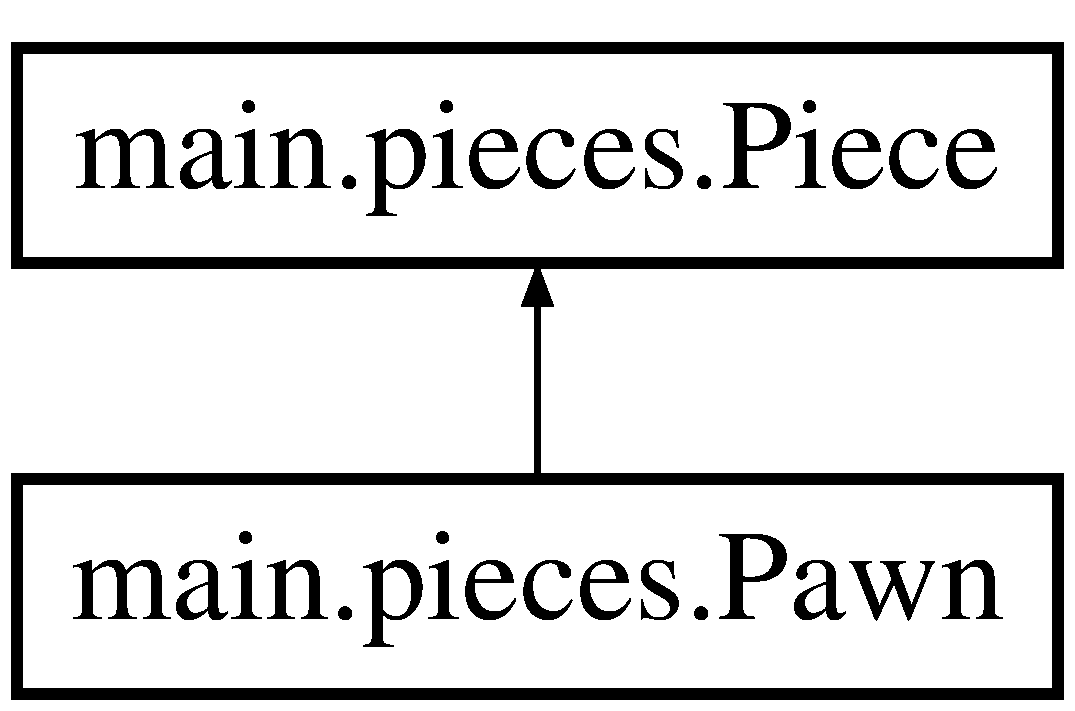
\includegraphics[height=2.000000cm]{classmain_1_1pieces_1_1_pawn}
\end{center}
\end{figure}
\subsection*{Public Member Functions}
\begin{DoxyCompactItemize}
\item 
\hyperlink{classmain_1_1pieces_1_1_pawn_ac0b9086627b2762dc851ae70945b0c9b}{Pawn} (int x, int y, String color)
\item 
String \hyperlink{classmain_1_1pieces_1_1_pawn_a5773cf85f79709da9dec92df7c98d64b}{get\+Type} ()
\item 
\hypertarget{classmain_1_1pieces_1_1_pawn_a9005e61dabd7be5a4755390cffda1709}{}\label{classmain_1_1pieces_1_1_pawn_a9005e61dabd7be5a4755390cffda1709} 
String {\bfseries to\+String} ()
\item 
Array\+List$<$ \hyperlink{classmain_1_1model_1_1_coordinate}{Coordinate} $>$ \hyperlink{classmain_1_1pieces_1_1_pawn_a06262375d095ccab099b861dc81bf5f1}{possible\+Moves} ()
\item 
void \hyperlink{classmain_1_1pieces_1_1_pawn_ae699e118a4a564de9d53839307f8aebe}{add\+Diagonal\+If\+Enemy\+Occupied} (Array\+List$<$ \hyperlink{classmain_1_1model_1_1_coordinate}{Coordinate} $>$ moves, int x, int y)
\end{DoxyCompactItemize}
\subsection*{Additional Inherited Members}


\subsection{Detailed Description}
Created by samir on 9/2/16. 

\subsection{Constructor \& Destructor Documentation}
\hypertarget{classmain_1_1pieces_1_1_pawn_ac0b9086627b2762dc851ae70945b0c9b}{}\label{classmain_1_1pieces_1_1_pawn_ac0b9086627b2762dc851ae70945b0c9b} 
\index{main\+::pieces\+::\+Pawn@{main\+::pieces\+::\+Pawn}!Pawn@{Pawn}}
\index{Pawn@{Pawn}!main\+::pieces\+::\+Pawn@{main\+::pieces\+::\+Pawn}}
\subsubsection{\texorpdfstring{Pawn()}{Pawn()}}
{\footnotesize\ttfamily main.\+pieces.\+Pawn.\+Pawn (\begin{DoxyParamCaption}\item[{int}]{x,  }\item[{int}]{y,  }\item[{String}]{color }\end{DoxyParamCaption})}

Constructor taking in x and y values for coordinates 

\subsection{Member Function Documentation}
\hypertarget{classmain_1_1pieces_1_1_pawn_ae699e118a4a564de9d53839307f8aebe}{}\label{classmain_1_1pieces_1_1_pawn_ae699e118a4a564de9d53839307f8aebe} 
\index{main\+::pieces\+::\+Pawn@{main\+::pieces\+::\+Pawn}!add\+Diagonal\+If\+Enemy\+Occupied@{add\+Diagonal\+If\+Enemy\+Occupied}}
\index{add\+Diagonal\+If\+Enemy\+Occupied@{add\+Diagonal\+If\+Enemy\+Occupied}!main\+::pieces\+::\+Pawn@{main\+::pieces\+::\+Pawn}}
\subsubsection{\texorpdfstring{add\+Diagonal\+If\+Enemy\+Occupied()}{addDiagonalIfEnemyOccupied()}}
{\footnotesize\ttfamily void main.\+pieces.\+Pawn.\+add\+Diagonal\+If\+Enemy\+Occupied (\begin{DoxyParamCaption}\item[{Array\+List$<$ \hyperlink{classmain_1_1model_1_1_coordinate}{Coordinate} $>$}]{moves,  }\item[{int}]{x,  }\item[{int}]{y }\end{DoxyParamCaption})}

Checks the pieces diagonally in front of the pawn for enemies If there are enemies, it is a valid move. Else, not a valid move. 
\begin{DoxyParams}{Parameters}
{\em moves} & \\
\hline
{\em x} & \\
\hline
{\em y} & \\
\hline
\end{DoxyParams}
\hypertarget{classmain_1_1pieces_1_1_pawn_a5773cf85f79709da9dec92df7c98d64b}{}\label{classmain_1_1pieces_1_1_pawn_a5773cf85f79709da9dec92df7c98d64b} 
\index{main\+::pieces\+::\+Pawn@{main\+::pieces\+::\+Pawn}!get\+Type@{get\+Type}}
\index{get\+Type@{get\+Type}!main\+::pieces\+::\+Pawn@{main\+::pieces\+::\+Pawn}}
\subsubsection{\texorpdfstring{get\+Type()}{getType()}}
{\footnotesize\ttfamily String main.\+pieces.\+Pawn.\+get\+Type (\begin{DoxyParamCaption}{ }\end{DoxyParamCaption})}

Returns the type of this piece \hypertarget{classmain_1_1pieces_1_1_pawn_a06262375d095ccab099b861dc81bf5f1}{}\label{classmain_1_1pieces_1_1_pawn_a06262375d095ccab099b861dc81bf5f1} 
\index{main\+::pieces\+::\+Pawn@{main\+::pieces\+::\+Pawn}!possible\+Moves@{possible\+Moves}}
\index{possible\+Moves@{possible\+Moves}!main\+::pieces\+::\+Pawn@{main\+::pieces\+::\+Pawn}}
\subsubsection{\texorpdfstring{possible\+Moves()}{possibleMoves()}}
{\footnotesize\ttfamily Array\+List$<$\hyperlink{classmain_1_1model_1_1_coordinate}{Coordinate}$>$ main.\+pieces.\+Pawn.\+possible\+Moves (\begin{DoxyParamCaption}{ }\end{DoxyParamCaption})}

Returns an Array\+List with the coordinates of the possible moves this pawn can make 

The documentation for this class was generated from the following file\+:\begin{DoxyCompactItemize}
\item 
src/main/pieces/Pawn.\+java\end{DoxyCompactItemize}

\hypertarget{classtests_1_1pieces_1_1_pawn_test}{}\section{tests.\+pieces.\+Pawn\+Test Class Reference}
\label{classtests_1_1pieces_1_1_pawn_test}\index{tests.\+pieces.\+Pawn\+Test@{tests.\+pieces.\+Pawn\+Test}}
\subsection*{Public Member Functions}
\begin{DoxyCompactItemize}
\item 
void \hyperlink{classtests_1_1pieces_1_1_pawn_test_a1c358f83062c1dcf97841cc61549d8f4}{valid\+Pawn\+Constructor} ()  throws Exception 
\item 
void \hyperlink{classtests_1_1pieces_1_1_pawn_test_a5f368d440aae4e9b128ed3a11b70bbc7}{valid\+Pawn\+Movement} ()  throws Exception 
\item 
void \hyperlink{classtests_1_1pieces_1_1_pawn_test_a2fd94e6381f006ac5ef2cf9b41974e3a}{invalid\+Pawn\+Movement} ()  throws Exception 
\end{DoxyCompactItemize}


\subsection{Detailed Description}
Created by samir on 9/3/16. 

\subsection{Member Function Documentation}
\hypertarget{classtests_1_1pieces_1_1_pawn_test_a2fd94e6381f006ac5ef2cf9b41974e3a}{}\label{classtests_1_1pieces_1_1_pawn_test_a2fd94e6381f006ac5ef2cf9b41974e3a} 
\index{tests\+::pieces\+::\+Pawn\+Test@{tests\+::pieces\+::\+Pawn\+Test}!invalid\+Pawn\+Movement@{invalid\+Pawn\+Movement}}
\index{invalid\+Pawn\+Movement@{invalid\+Pawn\+Movement}!tests\+::pieces\+::\+Pawn\+Test@{tests\+::pieces\+::\+Pawn\+Test}}
\subsubsection{\texorpdfstring{invalid\+Pawn\+Movement()}{invalidPawnMovement()}}
{\footnotesize\ttfamily void tests.\+pieces.\+Pawn\+Test.\+invalid\+Pawn\+Movement (\begin{DoxyParamCaption}{ }\end{DoxyParamCaption}) throws Exception}

c Test for invalid pawn movement if they have no available moves \hypertarget{classtests_1_1pieces_1_1_pawn_test_a1c358f83062c1dcf97841cc61549d8f4}{}\label{classtests_1_1pieces_1_1_pawn_test_a1c358f83062c1dcf97841cc61549d8f4} 
\index{tests\+::pieces\+::\+Pawn\+Test@{tests\+::pieces\+::\+Pawn\+Test}!valid\+Pawn\+Constructor@{valid\+Pawn\+Constructor}}
\index{valid\+Pawn\+Constructor@{valid\+Pawn\+Constructor}!tests\+::pieces\+::\+Pawn\+Test@{tests\+::pieces\+::\+Pawn\+Test}}
\subsubsection{\texorpdfstring{valid\+Pawn\+Constructor()}{validPawnConstructor()}}
{\footnotesize\ttfamily void tests.\+pieces.\+Pawn\+Test.\+valid\+Pawn\+Constructor (\begin{DoxyParamCaption}{ }\end{DoxyParamCaption}) throws Exception}

Valid constructor for a pawn should not throw an exception \hypertarget{classtests_1_1pieces_1_1_pawn_test_a5f368d440aae4e9b128ed3a11b70bbc7}{}\label{classtests_1_1pieces_1_1_pawn_test_a5f368d440aae4e9b128ed3a11b70bbc7} 
\index{tests\+::pieces\+::\+Pawn\+Test@{tests\+::pieces\+::\+Pawn\+Test}!valid\+Pawn\+Movement@{valid\+Pawn\+Movement}}
\index{valid\+Pawn\+Movement@{valid\+Pawn\+Movement}!tests\+::pieces\+::\+Pawn\+Test@{tests\+::pieces\+::\+Pawn\+Test}}
\subsubsection{\texorpdfstring{valid\+Pawn\+Movement()}{validPawnMovement()}}
{\footnotesize\ttfamily void tests.\+pieces.\+Pawn\+Test.\+valid\+Pawn\+Movement (\begin{DoxyParamCaption}{ }\end{DoxyParamCaption}) throws Exception}

Test for valid pawn movement (should be able to move) 

The documentation for this class was generated from the following file\+:\begin{DoxyCompactItemize}
\item 
src/tests/pieces/Pawn\+Test.\+java\end{DoxyCompactItemize}

\hypertarget{classmain_1_1pieces_1_1_piece}{}\section{main.\+pieces.\+Piece Class Reference}
\label{classmain_1_1pieces_1_1_piece}\index{main.\+pieces.\+Piece@{main.\+pieces.\+Piece}}
Inheritance diagram for main.\+pieces.\+Piece\+:\begin{figure}[H]
\begin{center}
\leavevmode
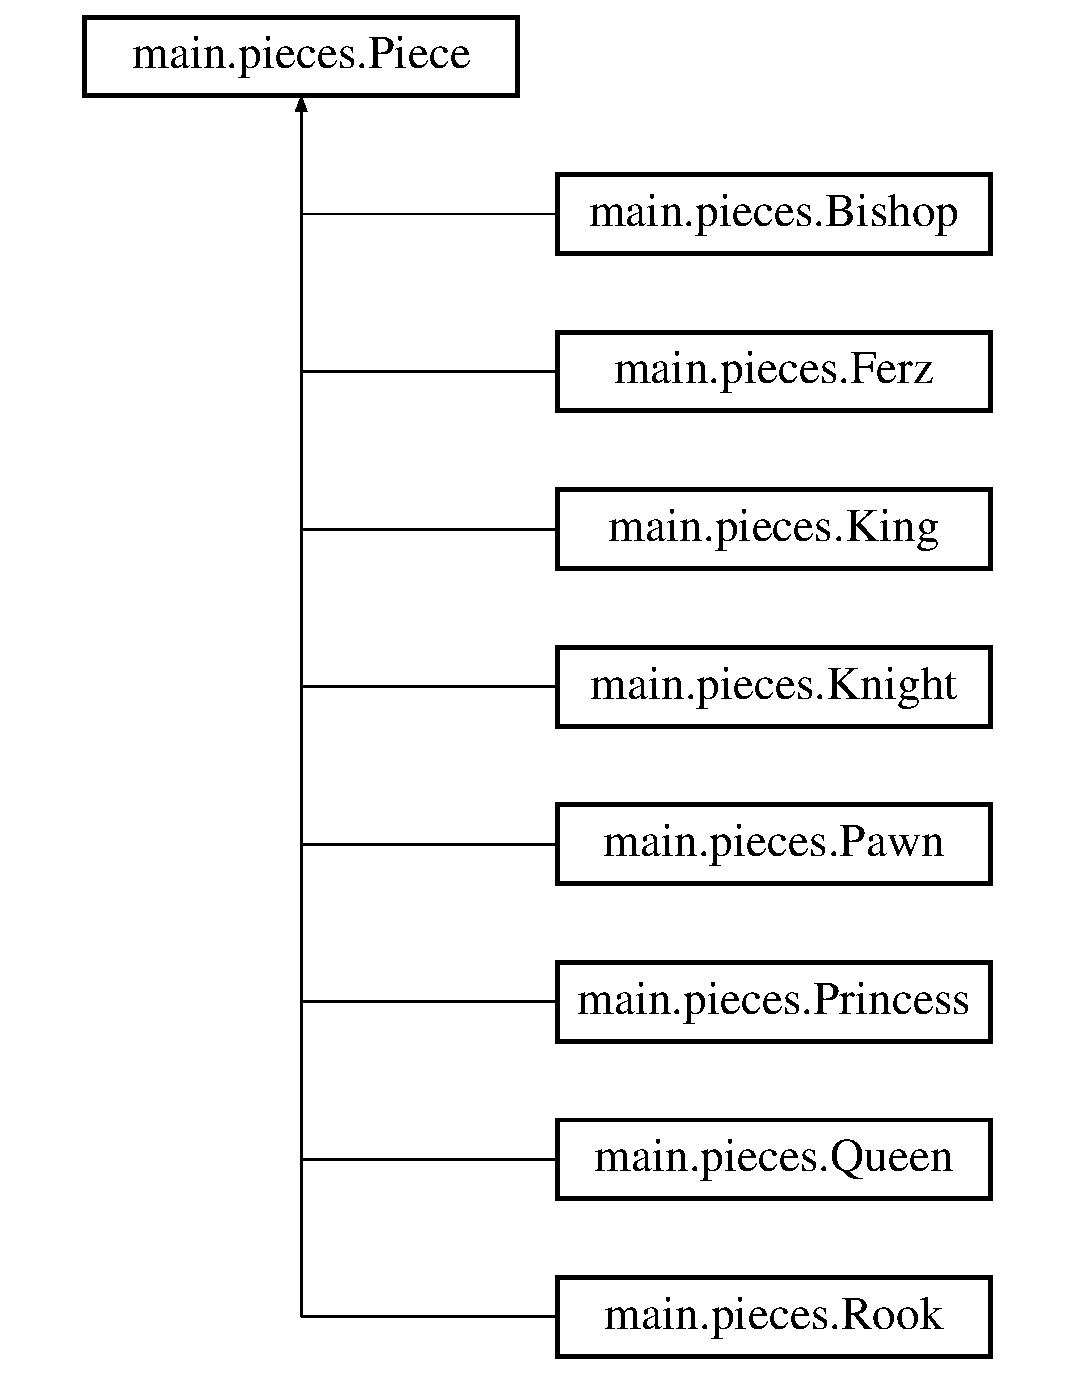
\includegraphics[height=9.000000cm]{classmain_1_1pieces_1_1_piece}
\end{center}
\end{figure}
\subsection*{Public Member Functions}
\begin{DoxyCompactItemize}
\item 
abstract Array\+List$<$ \hyperlink{classmain_1_1model_1_1_coordinate}{Coordinate} $>$ \hyperlink{classmain_1_1pieces_1_1_piece_a92a37b2f68604a6f2c8ece28d9a96080}{possible\+Moves} ()
\item 
abstract String \hyperlink{classmain_1_1pieces_1_1_piece_ae778ce746ff427326514c696cad72aba}{get\+Type} ()
\item 
abstract String \hyperlink{classmain_1_1pieces_1_1_piece_a528845eb51d394c21fd0f3d8a8011696}{to\+String} ()
\item 
String \hyperlink{classmain_1_1pieces_1_1_piece_a52545d99f7a6c36b99cfcf40fd0a9cef}{get\+Color} ()
\item 
\hypertarget{classmain_1_1pieces_1_1_piece_a2b808f44cec5a6b54ef073d1a89ea608}{}\label{classmain_1_1pieces_1_1_piece_a2b808f44cec5a6b54ef073d1a89ea608} 
void {\bfseries set\+Color} (String color)
\item 
\hypertarget{classmain_1_1pieces_1_1_piece_a69d998939d06b2bb749632864e0402b8}{}\label{classmain_1_1pieces_1_1_piece_a69d998939d06b2bb749632864e0402b8} 
\hyperlink{classmain_1_1model_1_1_coordinate}{Coordinate} {\bfseries get\+Coordinate} ()
\item 
\hypertarget{classmain_1_1pieces_1_1_piece_a7a6ab60bd575c3511957691989862745}{}\label{classmain_1_1pieces_1_1_piece_a7a6ab60bd575c3511957691989862745} 
void {\bfseries set\+Coordinate} (\hyperlink{classmain_1_1model_1_1_coordinate}{Coordinate} coordinate)
\item 
void \hyperlink{classmain_1_1pieces_1_1_piece_a2ffc0c01f80d164e8d471272061545d9}{set\+Coordinate} (int x, int y)
\item 
void \hyperlink{classmain_1_1pieces_1_1_piece_a58d0ca1c1f09ffd2470a4aec1b7e6854}{remove\+Piece} ()
\end{DoxyCompactItemize}
\subsection*{Public Attributes}
\begin{DoxyCompactItemize}
\item 
\hypertarget{classmain_1_1pieces_1_1_piece_a9f5e3f8b66b16fd732425936f63997ab}{}\label{classmain_1_1pieces_1_1_piece_a9f5e3f8b66b16fd732425936f63997ab} 
String {\bfseries image\+Path}
\end{DoxyCompactItemize}
\subsection*{Protected Member Functions}
\begin{DoxyCompactItemize}
\item 
void \hyperlink{classmain_1_1pieces_1_1_piece_aef1e0909297d1b3fd0974b4be25751c4}{check\+All\+Diagonals} (Array\+List$<$ \hyperlink{classmain_1_1model_1_1_coordinate}{Coordinate} $>$ moves, int x, int y)
\item 
void \hyperlink{classmain_1_1pieces_1_1_piece_ae50779c5a6de51ac05c6469e4660a82b}{check\+All\+Rows\+Columns} (Array\+List$<$ \hyperlink{classmain_1_1model_1_1_coordinate}{Coordinate} $>$ moves, int x, int y)
\item 
void \hyperlink{classmain_1_1pieces_1_1_piece_a12f2f0e6677148c31488ebf6a68cebaf}{add\+Coordinates\+In\+Direction} (Array\+List$<$ \hyperlink{classmain_1_1model_1_1_coordinate}{Coordinate} $>$ moves, int x, int y, int x\+Direction, int y\+Direction)
\item 
void \hyperlink{classmain_1_1pieces_1_1_piece_aae5cab0c47643b395e9c3050705b6fc9}{add\+Knight\+Coordinates} (Array\+List$<$ \hyperlink{classmain_1_1model_1_1_coordinate}{Coordinate} $>$ moves, int x, int y)
\item 
boolean \hyperlink{classmain_1_1pieces_1_1_piece_a74326d9253471ad25f8edb83bec207f6}{is\+Empty\+Coordinate} (int x, int y)
\item 
boolean \hyperlink{classmain_1_1pieces_1_1_piece_a164f24eb41f07fe4cb93d960f24d8638}{is\+Coordinate\+Available} (int x, int y)
\item 
boolean \hyperlink{classmain_1_1pieces_1_1_piece_a44b1600e3e49f6fdcd3dca288db82fd4}{add\+Coordinate\+If\+Available} (Array\+List$<$ \hyperlink{classmain_1_1model_1_1_coordinate}{Coordinate} $>$ moves, int x, int y)
\end{DoxyCompactItemize}


\subsection{Detailed Description}
Created by Samir on 9/1/16.

Idea box\+: Pieces remember how many other pieces it has taken (i.\+e. level up) 

\subsection{Member Function Documentation}
\hypertarget{classmain_1_1pieces_1_1_piece_a44b1600e3e49f6fdcd3dca288db82fd4}{}\label{classmain_1_1pieces_1_1_piece_a44b1600e3e49f6fdcd3dca288db82fd4} 
\index{main\+::pieces\+::\+Piece@{main\+::pieces\+::\+Piece}!add\+Coordinate\+If\+Available@{add\+Coordinate\+If\+Available}}
\index{add\+Coordinate\+If\+Available@{add\+Coordinate\+If\+Available}!main\+::pieces\+::\+Piece@{main\+::pieces\+::\+Piece}}
\subsubsection{\texorpdfstring{add\+Coordinate\+If\+Available()}{addCoordinateIfAvailable()}}
{\footnotesize\ttfamily boolean main.\+pieces.\+Piece.\+add\+Coordinate\+If\+Available (\begin{DoxyParamCaption}\item[{Array\+List$<$ \hyperlink{classmain_1_1model_1_1_coordinate}{Coordinate} $>$}]{moves,  }\item[{int}]{x,  }\item[{int}]{y }\end{DoxyParamCaption})\hspace{0.3cm}{\ttfamily [protected]}}

Adds the coordinate indicated by location (x,y) to the moves Array\+List if it is available \hypertarget{classmain_1_1pieces_1_1_piece_a12f2f0e6677148c31488ebf6a68cebaf}{}\label{classmain_1_1pieces_1_1_piece_a12f2f0e6677148c31488ebf6a68cebaf} 
\index{main\+::pieces\+::\+Piece@{main\+::pieces\+::\+Piece}!add\+Coordinates\+In\+Direction@{add\+Coordinates\+In\+Direction}}
\index{add\+Coordinates\+In\+Direction@{add\+Coordinates\+In\+Direction}!main\+::pieces\+::\+Piece@{main\+::pieces\+::\+Piece}}
\subsubsection{\texorpdfstring{add\+Coordinates\+In\+Direction()}{addCoordinatesInDirection()}}
{\footnotesize\ttfamily void main.\+pieces.\+Piece.\+add\+Coordinates\+In\+Direction (\begin{DoxyParamCaption}\item[{Array\+List$<$ \hyperlink{classmain_1_1model_1_1_coordinate}{Coordinate} $>$}]{moves,  }\item[{int}]{x,  }\item[{int}]{y,  }\item[{int}]{x\+Direction,  }\item[{int}]{y\+Direction }\end{DoxyParamCaption})\hspace{0.3cm}{\ttfamily [protected]}}

Check all the spaces in a direction given by x\+Direction and y\+Direction 
\begin{DoxyParams}{Parameters}
{\em moves} & \\
\hline
{\em x} & \\
\hline
{\em y} & \\
\hline
{\em x\+Direction} & -\/1, 0, or +1 to indicate negative, zero, or positive x-\/direction \\
\hline
{\em y\+Direction} & -\/1, 0, or +1 to indicate negative, zero, or positive y-\/direction \\
\hline
\end{DoxyParams}
\hypertarget{classmain_1_1pieces_1_1_piece_aae5cab0c47643b395e9c3050705b6fc9}{}\label{classmain_1_1pieces_1_1_piece_aae5cab0c47643b395e9c3050705b6fc9} 
\index{main\+::pieces\+::\+Piece@{main\+::pieces\+::\+Piece}!add\+Knight\+Coordinates@{add\+Knight\+Coordinates}}
\index{add\+Knight\+Coordinates@{add\+Knight\+Coordinates}!main\+::pieces\+::\+Piece@{main\+::pieces\+::\+Piece}}
\subsubsection{\texorpdfstring{add\+Knight\+Coordinates()}{addKnightCoordinates()}}
{\footnotesize\ttfamily void main.\+pieces.\+Piece.\+add\+Knight\+Coordinates (\begin{DoxyParamCaption}\item[{Array\+List$<$ \hyperlink{classmain_1_1model_1_1_coordinate}{Coordinate} $>$}]{moves,  }\item[{int}]{x,  }\item[{int}]{y }\end{DoxyParamCaption})\hspace{0.3cm}{\ttfamily [protected]}}

Adds the 8 possible positions a knight can move to 
\begin{DoxyParams}{Parameters}
{\em moves} & \\
\hline
{\em x} & \\
\hline
{\em y} & \\
\hline
\end{DoxyParams}
\hypertarget{classmain_1_1pieces_1_1_piece_aef1e0909297d1b3fd0974b4be25751c4}{}\label{classmain_1_1pieces_1_1_piece_aef1e0909297d1b3fd0974b4be25751c4} 
\index{main\+::pieces\+::\+Piece@{main\+::pieces\+::\+Piece}!check\+All\+Diagonals@{check\+All\+Diagonals}}
\index{check\+All\+Diagonals@{check\+All\+Diagonals}!main\+::pieces\+::\+Piece@{main\+::pieces\+::\+Piece}}
\subsubsection{\texorpdfstring{check\+All\+Diagonals()}{checkAllDiagonals()}}
{\footnotesize\ttfamily void main.\+pieces.\+Piece.\+check\+All\+Diagonals (\begin{DoxyParamCaption}\item[{Array\+List$<$ \hyperlink{classmain_1_1model_1_1_coordinate}{Coordinate} $>$}]{moves,  }\item[{int}]{x,  }\item[{int}]{y }\end{DoxyParamCaption})\hspace{0.3cm}{\ttfamily [protected]}}

\subparagraph*{}

Move Methods \subparagraph*{}

Checks all the spaces diagonal to the location given by (x,y) and adds them to the moves Array\+List if they are available 
\begin{DoxyParams}{Parameters}
{\em moves} & \\
\hline
{\em x} & \\
\hline
{\em y} & \\
\hline
\end{DoxyParams}
\hypertarget{classmain_1_1pieces_1_1_piece_ae50779c5a6de51ac05c6469e4660a82b}{}\label{classmain_1_1pieces_1_1_piece_ae50779c5a6de51ac05c6469e4660a82b} 
\index{main\+::pieces\+::\+Piece@{main\+::pieces\+::\+Piece}!check\+All\+Rows\+Columns@{check\+All\+Rows\+Columns}}
\index{check\+All\+Rows\+Columns@{check\+All\+Rows\+Columns}!main\+::pieces\+::\+Piece@{main\+::pieces\+::\+Piece}}
\subsubsection{\texorpdfstring{check\+All\+Rows\+Columns()}{checkAllRowsColumns()}}
{\footnotesize\ttfamily void main.\+pieces.\+Piece.\+check\+All\+Rows\+Columns (\begin{DoxyParamCaption}\item[{Array\+List$<$ \hyperlink{classmain_1_1model_1_1_coordinate}{Coordinate} $>$}]{moves,  }\item[{int}]{x,  }\item[{int}]{y }\end{DoxyParamCaption})\hspace{0.3cm}{\ttfamily [protected]}}

Checks all the spaces in the same row and column to the location given by (x,y) and adds them to the moves Array\+List if they are available 
\begin{DoxyParams}{Parameters}
{\em moves} & \\
\hline
{\em x} & \\
\hline
{\em y} & \\
\hline
\end{DoxyParams}
\hypertarget{classmain_1_1pieces_1_1_piece_a52545d99f7a6c36b99cfcf40fd0a9cef}{}\label{classmain_1_1pieces_1_1_piece_a52545d99f7a6c36b99cfcf40fd0a9cef} 
\index{main\+::pieces\+::\+Piece@{main\+::pieces\+::\+Piece}!get\+Color@{get\+Color}}
\index{get\+Color@{get\+Color}!main\+::pieces\+::\+Piece@{main\+::pieces\+::\+Piece}}
\subsubsection{\texorpdfstring{get\+Color()}{getColor()}}
{\footnotesize\ttfamily String main.\+pieces.\+Piece.\+get\+Color (\begin{DoxyParamCaption}{ }\end{DoxyParamCaption})}

\subparagraph*{}

Getter/\+Setter Methods \subparagraph*{}\hypertarget{classmain_1_1pieces_1_1_piece_ae778ce746ff427326514c696cad72aba}{}\label{classmain_1_1pieces_1_1_piece_ae778ce746ff427326514c696cad72aba} 
\index{main\+::pieces\+::\+Piece@{main\+::pieces\+::\+Piece}!get\+Type@{get\+Type}}
\index{get\+Type@{get\+Type}!main\+::pieces\+::\+Piece@{main\+::pieces\+::\+Piece}}
\subsubsection{\texorpdfstring{get\+Type()}{getType()}}
{\footnotesize\ttfamily abstract String main.\+pieces.\+Piece.\+get\+Type (\begin{DoxyParamCaption}{ }\end{DoxyParamCaption})\hspace{0.3cm}{\ttfamily [abstract]}}

Return the type of the piece \begin{DoxyReturn}{Returns}

\end{DoxyReturn}
\hypertarget{classmain_1_1pieces_1_1_piece_a164f24eb41f07fe4cb93d960f24d8638}{}\label{classmain_1_1pieces_1_1_piece_a164f24eb41f07fe4cb93d960f24d8638} 
\index{main\+::pieces\+::\+Piece@{main\+::pieces\+::\+Piece}!is\+Coordinate\+Available@{is\+Coordinate\+Available}}
\index{is\+Coordinate\+Available@{is\+Coordinate\+Available}!main\+::pieces\+::\+Piece@{main\+::pieces\+::\+Piece}}
\subsubsection{\texorpdfstring{is\+Coordinate\+Available()}{isCoordinateAvailable()}}
{\footnotesize\ttfamily boolean main.\+pieces.\+Piece.\+is\+Coordinate\+Available (\begin{DoxyParamCaption}\item[{int}]{x,  }\item[{int}]{y }\end{DoxyParamCaption})\hspace{0.3cm}{\ttfamily [protected]}}

Checks the space to see if its available or occupied by opposing piece \begin{DoxyReturn}{Returns}
A coordinate for the space if it is available 
\end{DoxyReturn}
\hypertarget{classmain_1_1pieces_1_1_piece_a74326d9253471ad25f8edb83bec207f6}{}\label{classmain_1_1pieces_1_1_piece_a74326d9253471ad25f8edb83bec207f6} 
\index{main\+::pieces\+::\+Piece@{main\+::pieces\+::\+Piece}!is\+Empty\+Coordinate@{is\+Empty\+Coordinate}}
\index{is\+Empty\+Coordinate@{is\+Empty\+Coordinate}!main\+::pieces\+::\+Piece@{main\+::pieces\+::\+Piece}}
\subsubsection{\texorpdfstring{is\+Empty\+Coordinate()}{isEmptyCoordinate()}}
{\footnotesize\ttfamily boolean main.\+pieces.\+Piece.\+is\+Empty\+Coordinate (\begin{DoxyParamCaption}\item[{int}]{x,  }\item[{int}]{y }\end{DoxyParamCaption})\hspace{0.3cm}{\ttfamily [protected]}}

Return true/false if the coordinate is unoccupied 
\begin{DoxyParams}{Parameters}
{\em x} & \\
\hline
{\em y} & \\
\hline
\end{DoxyParams}
\begin{DoxyReturn}{Returns}

\end{DoxyReturn}
\hypertarget{classmain_1_1pieces_1_1_piece_a92a37b2f68604a6f2c8ece28d9a96080}{}\label{classmain_1_1pieces_1_1_piece_a92a37b2f68604a6f2c8ece28d9a96080} 
\index{main\+::pieces\+::\+Piece@{main\+::pieces\+::\+Piece}!possible\+Moves@{possible\+Moves}}
\index{possible\+Moves@{possible\+Moves}!main\+::pieces\+::\+Piece@{main\+::pieces\+::\+Piece}}
\subsubsection{\texorpdfstring{possible\+Moves()}{possibleMoves()}}
{\footnotesize\ttfamily abstract Array\+List$<$\hyperlink{classmain_1_1model_1_1_coordinate}{Coordinate}$>$ main.\+pieces.\+Piece.\+possible\+Moves (\begin{DoxyParamCaption}{ }\end{DoxyParamCaption})\hspace{0.3cm}{\ttfamily [abstract]}}

\subparagraph*{}

Abstract Methods \subparagraph*{}

Return an arraylist of coordinates of all the possible moves this piece can make \begin{DoxyReturn}{Returns}

\end{DoxyReturn}
\hypertarget{classmain_1_1pieces_1_1_piece_a58d0ca1c1f09ffd2470a4aec1b7e6854}{}\label{classmain_1_1pieces_1_1_piece_a58d0ca1c1f09ffd2470a4aec1b7e6854} 
\index{main\+::pieces\+::\+Piece@{main\+::pieces\+::\+Piece}!remove\+Piece@{remove\+Piece}}
\index{remove\+Piece@{remove\+Piece}!main\+::pieces\+::\+Piece@{main\+::pieces\+::\+Piece}}
\subsubsection{\texorpdfstring{remove\+Piece()}{removePiece()}}
{\footnotesize\ttfamily void main.\+pieces.\+Piece.\+remove\+Piece (\begin{DoxyParamCaption}{ }\end{DoxyParamCaption})}

Sets the pieces coordinates to null \hypertarget{classmain_1_1pieces_1_1_piece_a2ffc0c01f80d164e8d471272061545d9}{}\label{classmain_1_1pieces_1_1_piece_a2ffc0c01f80d164e8d471272061545d9} 
\index{main\+::pieces\+::\+Piece@{main\+::pieces\+::\+Piece}!set\+Coordinate@{set\+Coordinate}}
\index{set\+Coordinate@{set\+Coordinate}!main\+::pieces\+::\+Piece@{main\+::pieces\+::\+Piece}}
\subsubsection{\texorpdfstring{set\+Coordinate()}{setCoordinate()}}
{\footnotesize\ttfamily void main.\+pieces.\+Piece.\+set\+Coordinate (\begin{DoxyParamCaption}\item[{int}]{x,  }\item[{int}]{y }\end{DoxyParamCaption})}

\subparagraph*{}

Coordinate Methods \subparagraph*{}

Update the coordinates of the piece \hypertarget{classmain_1_1pieces_1_1_piece_a528845eb51d394c21fd0f3d8a8011696}{}\label{classmain_1_1pieces_1_1_piece_a528845eb51d394c21fd0f3d8a8011696} 
\index{main\+::pieces\+::\+Piece@{main\+::pieces\+::\+Piece}!to\+String@{to\+String}}
\index{to\+String@{to\+String}!main\+::pieces\+::\+Piece@{main\+::pieces\+::\+Piece}}
\subsubsection{\texorpdfstring{to\+String()}{toString()}}
{\footnotesize\ttfamily abstract String main.\+pieces.\+Piece.\+to\+String (\begin{DoxyParamCaption}{ }\end{DoxyParamCaption})\hspace{0.3cm}{\ttfamily [abstract]}}

Return the string representation of the piece \begin{DoxyReturn}{Returns}

\end{DoxyReturn}


The documentation for this class was generated from the following file\+:\begin{DoxyCompactItemize}
\item 
src/main/pieces/Piece.\+java\end{DoxyCompactItemize}

\hypertarget{classtests_1_1pieces_1_1_piece_test}{}\section{tests.\+pieces.\+Piece\+Test Class Reference}
\label{classtests_1_1pieces_1_1_piece_test}\index{tests.\+pieces.\+Piece\+Test@{tests.\+pieces.\+Piece\+Test}}
\subsection*{Public Member Functions}
\begin{DoxyCompactItemize}
\item 
\hypertarget{classtests_1_1pieces_1_1_piece_test_a51a3855c40d3da846cd11f8fc6881471}{}\label{classtests_1_1pieces_1_1_piece_test_a51a3855c40d3da846cd11f8fc6881471} 
void {\bfseries capture\+A\+Piece} ()  throws Exception 
\end{DoxyCompactItemize}


\subsection{Detailed Description}
Created by samir on 9/3/16. 

The documentation for this class was generated from the following file\+:\begin{DoxyCompactItemize}
\item 
src/tests/pieces/Piece\+Test.\+java\end{DoxyCompactItemize}

\hypertarget{classmain_1_1_player}{}\section{main.\+Player Class Reference}
\label{classmain_1_1_player}\index{main.\+Player@{main.\+Player}}
\subsection*{Public Member Functions}
\begin{DoxyCompactItemize}
\item 
\hyperlink{classmain_1_1_player_a7a07b12fa4f52134a9b68abf32b0cb65}{Player} (String color, String name)
\item 
void \hyperlink{classmain_1_1_player_a0ab2e50adb7dd825ae62268459dfb633}{reset\+State} ()
\item 
void \hyperlink{classmain_1_1_player_a20e4d2604d95857e73ba9ce628b2037b}{check\+Board\+Status} (\hyperlink{classmain_1_1_board_view}{Board\+View} board\+View, \hyperlink{classmain_1_1model_1_1_board}{Board} board)
\end{DoxyCompactItemize}
\subsection*{Static Public Member Functions}
\begin{DoxyCompactItemize}
\item 
static boolean \hyperlink{classmain_1_1_player_a154e7eebeeab65000f917c736f6cb822}{validate\+Piece} (\hyperlink{classmain_1_1pieces_1_1_piece}{Piece} piece, String color, \hyperlink{classmain_1_1_board_view}{Board\+View} board\+View, \hyperlink{classmain_1_1pieces_1_1_piece}{Piece} selected\+Piece)
\end{DoxyCompactItemize}
\subsection*{Public Attributes}
\begin{DoxyCompactItemize}
\item 
\hypertarget{classmain_1_1_player_a676bda6b0543e4e4093955835f1829da}{}\label{classmain_1_1_player_a676bda6b0543e4e4093955835f1829da} 
String {\bfseries color}
\item 
\hypertarget{classmain_1_1_player_a3214a3ccfb412f6418cb30629efbdba8}{}\label{classmain_1_1_player_a3214a3ccfb412f6418cb30629efbdba8} 
boolean {\bfseries check}
\item 
\hypertarget{classmain_1_1_player_a37183b7b9911bca48917a4d560fb5a08}{}\label{classmain_1_1_player_a37183b7b9911bca48917a4d560fb5a08} 
boolean {\bfseries check\+Mate}
\item 
\hypertarget{classmain_1_1_player_a789e767891852d4225dd3374d8c1507d}{}\label{classmain_1_1_player_a789e767891852d4225dd3374d8c1507d} 
int {\bfseries score}
\item 
\hypertarget{classmain_1_1_player_a52da3f9931858dcde58a377923e98073}{}\label{classmain_1_1_player_a52da3f9931858dcde58a377923e98073} 
String {\bfseries name}
\end{DoxyCompactItemize}


\subsection{Detailed Description}
Created by samir on 9/5/16. 

\subsection{Constructor \& Destructor Documentation}
\hypertarget{classmain_1_1_player_a7a07b12fa4f52134a9b68abf32b0cb65}{}\label{classmain_1_1_player_a7a07b12fa4f52134a9b68abf32b0cb65} 
\index{main\+::\+Player@{main\+::\+Player}!Player@{Player}}
\index{Player@{Player}!main\+::\+Player@{main\+::\+Player}}
\subsubsection{\texorpdfstring{Player()}{Player()}}
{\footnotesize\ttfamily main.\+Player.\+Player (\begin{DoxyParamCaption}\item[{String}]{color,  }\item[{String}]{name }\end{DoxyParamCaption})}

\hyperlink{classmain_1_1_player}{Player} constructor 
\begin{DoxyParams}{Parameters}
{\em color} & \\
\hline
{\em name} & \\
\hline
\end{DoxyParams}


\subsection{Member Function Documentation}
\hypertarget{classmain_1_1_player_a20e4d2604d95857e73ba9ce628b2037b}{}\label{classmain_1_1_player_a20e4d2604d95857e73ba9ce628b2037b} 
\index{main\+::\+Player@{main\+::\+Player}!check\+Board\+Status@{check\+Board\+Status}}
\index{check\+Board\+Status@{check\+Board\+Status}!main\+::\+Player@{main\+::\+Player}}
\subsubsection{\texorpdfstring{check\+Board\+Status()}{checkBoardStatus()}}
{\footnotesize\ttfamily void main.\+Player.\+check\+Board\+Status (\begin{DoxyParamCaption}\item[{\hyperlink{classmain_1_1_board_view}{Board\+View}}]{board\+View,  }\item[{\hyperlink{classmain_1_1model_1_1_board}{Board}}]{board }\end{DoxyParamCaption})}

Checks the board\+G\+UI after a move to see if the move placed this player in check or checkmate 
\begin{DoxyParams}{Parameters}
{\em board\+View} & \\
\hline
{\em board} & \\
\hline
\end{DoxyParams}
\hypertarget{classmain_1_1_player_a0ab2e50adb7dd825ae62268459dfb633}{}\label{classmain_1_1_player_a0ab2e50adb7dd825ae62268459dfb633} 
\index{main\+::\+Player@{main\+::\+Player}!reset\+State@{reset\+State}}
\index{reset\+State@{reset\+State}!main\+::\+Player@{main\+::\+Player}}
\subsubsection{\texorpdfstring{reset\+State()}{resetState()}}
{\footnotesize\ttfamily void main.\+Player.\+reset\+State (\begin{DoxyParamCaption}{ }\end{DoxyParamCaption})}

Reset the check and checkmate state of this player \hypertarget{classmain_1_1_player_a154e7eebeeab65000f917c736f6cb822}{}\label{classmain_1_1_player_a154e7eebeeab65000f917c736f6cb822} 
\index{main\+::\+Player@{main\+::\+Player}!validate\+Piece@{validate\+Piece}}
\index{validate\+Piece@{validate\+Piece}!main\+::\+Player@{main\+::\+Player}}
\subsubsection{\texorpdfstring{validate\+Piece()}{validatePiece()}}
{\footnotesize\ttfamily static boolean main.\+Player.\+validate\+Piece (\begin{DoxyParamCaption}\item[{\hyperlink{classmain_1_1pieces_1_1_piece}{Piece}}]{piece,  }\item[{String}]{color,  }\item[{\hyperlink{classmain_1_1_board_view}{Board\+View}}]{board\+View,  }\item[{\hyperlink{classmain_1_1pieces_1_1_piece}{Piece}}]{selected\+Piece }\end{DoxyParamCaption})\hspace{0.3cm}{\ttfamily [static]}}

Validates that the piece at the given coordinate is a valid piece that the player controls If not valid, alert the player with the corresponding message 
\begin{DoxyParams}{Parameters}
{\em piece} & \\
\hline
{\em color} & \\
\hline
{\em board\+View} & \\
\hline
{\em selected\+Piece} & \\
\hline
\end{DoxyParams}
\begin{DoxyReturn}{Returns}
True if valid, False if not 
\end{DoxyReturn}


The documentation for this class was generated from the following file\+:\begin{DoxyCompactItemize}
\item 
src/main/Player.\+java\end{DoxyCompactItemize}

\hypertarget{classtests_1_1game_1_1_player_test}{}\section{tests.\+game.\+Player\+Test Class Reference}
\label{classtests_1_1game_1_1_player_test}\index{tests.\+game.\+Player\+Test@{tests.\+game.\+Player\+Test}}
\subsection*{Public Member Functions}
\begin{DoxyCompactItemize}
\item 
\hypertarget{classtests_1_1game_1_1_player_test_a94606fac06d2cd22b1c945ae5b0b6bdb}{}\label{classtests_1_1game_1_1_player_test_a94606fac06d2cd22b1c945ae5b0b6bdb} 
void {\bfseries valid\+Player\+Constructor} ()  throws Exception 
\item 
\hypertarget{classtests_1_1game_1_1_player_test_a214a608d362d72b11ea55eb86af41718}{}\label{classtests_1_1game_1_1_player_test_a214a608d362d72b11ea55eb86af41718} 
void {\bfseries reset\+Player\+State} ()  throws Exception 
\end{DoxyCompactItemize}


\subsection{Detailed Description}
Created by samir on 9/21/16. 

The documentation for this class was generated from the following file\+:\begin{DoxyCompactItemize}
\item 
src/tests/game/Player\+Test.\+java\end{DoxyCompactItemize}

\hypertarget{classmain_1_1pieces_1_1_princess}{}\section{main.\+pieces.\+Princess Class Reference}
\label{classmain_1_1pieces_1_1_princess}\index{main.\+pieces.\+Princess@{main.\+pieces.\+Princess}}
Inheritance diagram for main.\+pieces.\+Princess\+:\begin{figure}[H]
\begin{center}
\leavevmode
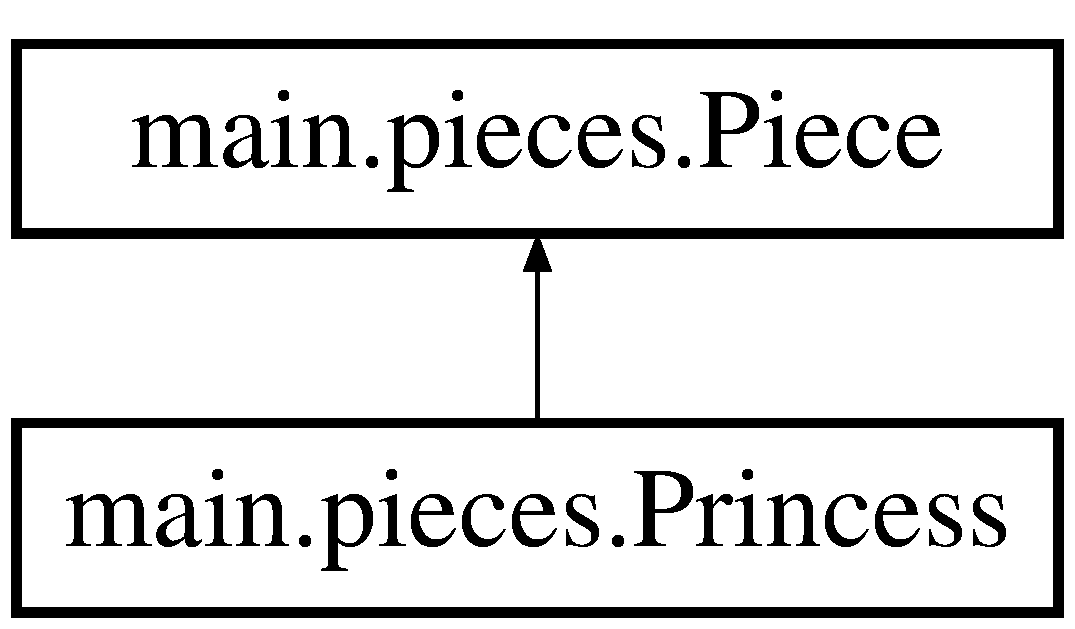
\includegraphics[height=2.000000cm]{classmain_1_1pieces_1_1_princess}
\end{center}
\end{figure}
\subsection*{Public Member Functions}
\begin{DoxyCompactItemize}
\item 
\hyperlink{classmain_1_1pieces_1_1_princess_a971505387339fcf55d55296b0f479cc3}{Princess} (String color)
\item 
String \hyperlink{classmain_1_1pieces_1_1_princess_a63a4459d73ae413757873769a0a66691}{get\+Type} ()
\item 
String \hyperlink{classmain_1_1pieces_1_1_princess_a8be1df155dee4a3fbcc4ae1eebea0ff4}{to\+String} ()
\item 
Array\+List$<$ \hyperlink{classmain_1_1model_1_1_coordinate}{Coordinate} $>$ \hyperlink{classmain_1_1pieces_1_1_princess_a77559cdb19a3fdd60237bddef0420b44}{possible\+Moves} ()
\end{DoxyCompactItemize}
\subsection*{Additional Inherited Members}


\subsection{Detailed Description}
Created by samir on 9/13/16. 

\subsection{Constructor \& Destructor Documentation}
\hypertarget{classmain_1_1pieces_1_1_princess_a971505387339fcf55d55296b0f479cc3}{}\label{classmain_1_1pieces_1_1_princess_a971505387339fcf55d55296b0f479cc3} 
\index{main\+::pieces\+::\+Princess@{main\+::pieces\+::\+Princess}!Princess@{Princess}}
\index{Princess@{Princess}!main\+::pieces\+::\+Princess@{main\+::pieces\+::\+Princess}}
\subsubsection{\texorpdfstring{Princess()}{Princess()}}
{\footnotesize\ttfamily main.\+pieces.\+Princess.\+Princess (\begin{DoxyParamCaption}\item[{String}]{color }\end{DoxyParamCaption})}

\hyperlink{classmain_1_1pieces_1_1_princess}{Princess} constructor 
\begin{DoxyParams}{Parameters}
{\em color} & \\
\hline
\end{DoxyParams}


\subsection{Member Function Documentation}
\hypertarget{classmain_1_1pieces_1_1_princess_a63a4459d73ae413757873769a0a66691}{}\label{classmain_1_1pieces_1_1_princess_a63a4459d73ae413757873769a0a66691} 
\index{main\+::pieces\+::\+Princess@{main\+::pieces\+::\+Princess}!get\+Type@{get\+Type}}
\index{get\+Type@{get\+Type}!main\+::pieces\+::\+Princess@{main\+::pieces\+::\+Princess}}
\subsubsection{\texorpdfstring{get\+Type()}{getType()}}
{\footnotesize\ttfamily String main.\+pieces.\+Princess.\+get\+Type (\begin{DoxyParamCaption}{ }\end{DoxyParamCaption})}

Return the type of piece \begin{DoxyReturn}{Returns}

\end{DoxyReturn}
\hypertarget{classmain_1_1pieces_1_1_princess_a77559cdb19a3fdd60237bddef0420b44}{}\label{classmain_1_1pieces_1_1_princess_a77559cdb19a3fdd60237bddef0420b44} 
\index{main\+::pieces\+::\+Princess@{main\+::pieces\+::\+Princess}!possible\+Moves@{possible\+Moves}}
\index{possible\+Moves@{possible\+Moves}!main\+::pieces\+::\+Princess@{main\+::pieces\+::\+Princess}}
\subsubsection{\texorpdfstring{possible\+Moves()}{possibleMoves()}}
{\footnotesize\ttfamily Array\+List$<$\hyperlink{classmain_1_1model_1_1_coordinate}{Coordinate}$>$ main.\+pieces.\+Princess.\+possible\+Moves (\begin{DoxyParamCaption}{ }\end{DoxyParamCaption})}

Return an Array\+List of Coordinates of possible moves the \hyperlink{classmain_1_1pieces_1_1_ferz}{Ferz} can make \begin{DoxyReturn}{Returns}

\end{DoxyReturn}
\hypertarget{classmain_1_1pieces_1_1_princess_a8be1df155dee4a3fbcc4ae1eebea0ff4}{}\label{classmain_1_1pieces_1_1_princess_a8be1df155dee4a3fbcc4ae1eebea0ff4} 
\index{main\+::pieces\+::\+Princess@{main\+::pieces\+::\+Princess}!to\+String@{to\+String}}
\index{to\+String@{to\+String}!main\+::pieces\+::\+Princess@{main\+::pieces\+::\+Princess}}
\subsubsection{\texorpdfstring{to\+String()}{toString()}}
{\footnotesize\ttfamily String main.\+pieces.\+Princess.\+to\+String (\begin{DoxyParamCaption}{ }\end{DoxyParamCaption})}

String representation of a \hyperlink{classmain_1_1pieces_1_1_ferz}{Ferz} \begin{DoxyReturn}{Returns}

\end{DoxyReturn}


The documentation for this class was generated from the following file\+:\begin{DoxyCompactItemize}
\item 
src/main/pieces/Princess.\+java\end{DoxyCompactItemize}

\hypertarget{classtests_1_1pieces_1_1_princess_test}{}\section{tests.\+pieces.\+Princess\+Test Class Reference}
\label{classtests_1_1pieces_1_1_princess_test}\index{tests.\+pieces.\+Princess\+Test@{tests.\+pieces.\+Princess\+Test}}
\subsection*{Public Member Functions}
\begin{DoxyCompactItemize}
\item 
\hypertarget{classtests_1_1pieces_1_1_princess_test_a43a248493cdd9ca69cb18290e3061167}{}\label{classtests_1_1pieces_1_1_princess_test_a43a248493cdd9ca69cb18290e3061167} 
void {\bfseries valid\+Princess\+Constructor} ()  throws Exception 
\item 
\hypertarget{classtests_1_1pieces_1_1_princess_test_af768e952940e3234a54be9b40a2ea0f5}{}\label{classtests_1_1pieces_1_1_princess_test_af768e952940e3234a54be9b40a2ea0f5} 
void {\bfseries valid\+Princess\+Movement} ()  throws Exception 
\end{DoxyCompactItemize}


\subsection{Detailed Description}
Created by samir on 9/13/16. 

The documentation for this class was generated from the following file\+:\begin{DoxyCompactItemize}
\item 
src/tests/pieces/Princess\+Test.\+java\end{DoxyCompactItemize}

\hypertarget{classmain_1_1pieces_1_1_queen}{}\section{main.\+pieces.\+Queen Class Reference}
\label{classmain_1_1pieces_1_1_queen}\index{main.\+pieces.\+Queen@{main.\+pieces.\+Queen}}
Inheritance diagram for main.\+pieces.\+Queen\+:\begin{figure}[H]
\begin{center}
\leavevmode
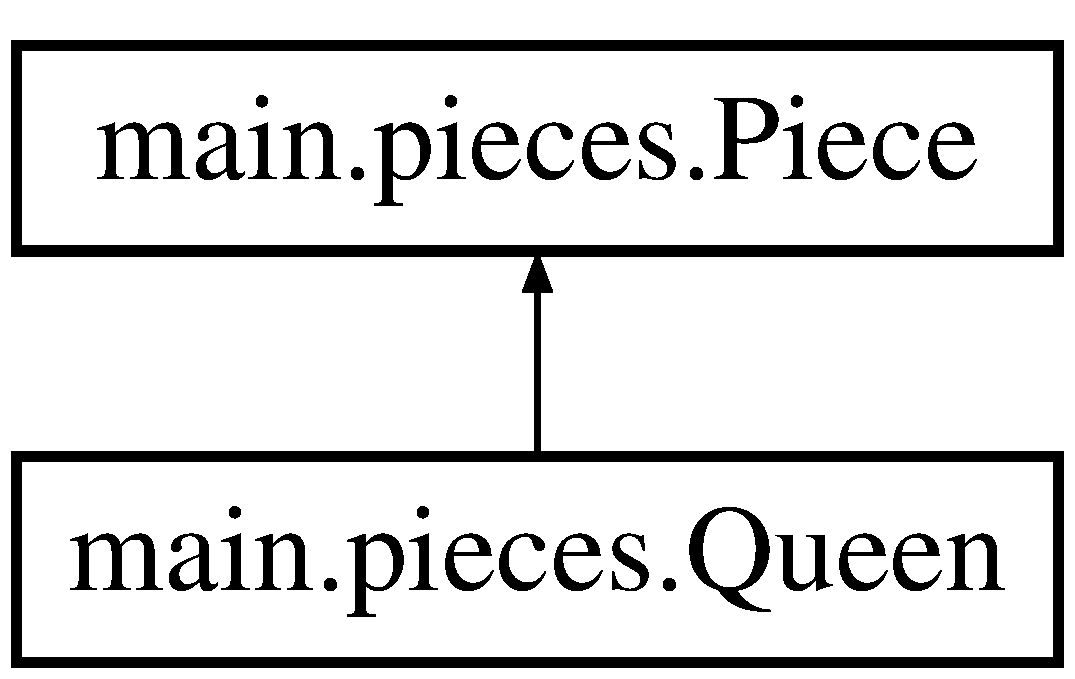
\includegraphics[height=2.000000cm]{classmain_1_1pieces_1_1_queen}
\end{center}
\end{figure}
\subsection*{Public Member Functions}
\begin{DoxyCompactItemize}
\item 
\hyperlink{classmain_1_1pieces_1_1_queen_ac013f2c9aa2e24f6633d41711a83ff1e}{Queen} (String color)
\item 
String \hyperlink{classmain_1_1pieces_1_1_queen_a7964928ca1ea3ecfaa04d80dc5764d5b}{get\+Type} ()
\item 
String \hyperlink{classmain_1_1pieces_1_1_queen_a87b715eb4a56c840d1e1830264d23a56}{to\+String} ()
\item 
Array\+List$<$ \hyperlink{classmain_1_1model_1_1_coordinate}{Coordinate} $>$ \hyperlink{classmain_1_1pieces_1_1_queen_a8791ac2f814bb5d3791c7787e2714b9e}{possible\+Moves} ()
\end{DoxyCompactItemize}
\subsection*{Additional Inherited Members}


\subsection{Detailed Description}
Created by Samir on 9/3/16. 

\subsection{Constructor \& Destructor Documentation}
\hypertarget{classmain_1_1pieces_1_1_queen_ac013f2c9aa2e24f6633d41711a83ff1e}{}\label{classmain_1_1pieces_1_1_queen_ac013f2c9aa2e24f6633d41711a83ff1e} 
\index{main\+::pieces\+::\+Queen@{main\+::pieces\+::\+Queen}!Queen@{Queen}}
\index{Queen@{Queen}!main\+::pieces\+::\+Queen@{main\+::pieces\+::\+Queen}}
\subsubsection{\texorpdfstring{Queen()}{Queen()}}
{\footnotesize\ttfamily main.\+pieces.\+Queen.\+Queen (\begin{DoxyParamCaption}\item[{String}]{color }\end{DoxyParamCaption})}

Constructor taking in the queen\textquotesingle{}s color 

\subsection{Member Function Documentation}
\hypertarget{classmain_1_1pieces_1_1_queen_a7964928ca1ea3ecfaa04d80dc5764d5b}{}\label{classmain_1_1pieces_1_1_queen_a7964928ca1ea3ecfaa04d80dc5764d5b} 
\index{main\+::pieces\+::\+Queen@{main\+::pieces\+::\+Queen}!get\+Type@{get\+Type}}
\index{get\+Type@{get\+Type}!main\+::pieces\+::\+Queen@{main\+::pieces\+::\+Queen}}
\subsubsection{\texorpdfstring{get\+Type()}{getType()}}
{\footnotesize\ttfamily String main.\+pieces.\+Queen.\+get\+Type (\begin{DoxyParamCaption}{ }\end{DoxyParamCaption})}

Returns the type of this piece \hypertarget{classmain_1_1pieces_1_1_queen_a8791ac2f814bb5d3791c7787e2714b9e}{}\label{classmain_1_1pieces_1_1_queen_a8791ac2f814bb5d3791c7787e2714b9e} 
\index{main\+::pieces\+::\+Queen@{main\+::pieces\+::\+Queen}!possible\+Moves@{possible\+Moves}}
\index{possible\+Moves@{possible\+Moves}!main\+::pieces\+::\+Queen@{main\+::pieces\+::\+Queen}}
\subsubsection{\texorpdfstring{possible\+Moves()}{possibleMoves()}}
{\footnotesize\ttfamily Array\+List$<$\hyperlink{classmain_1_1model_1_1_coordinate}{Coordinate}$>$ main.\+pieces.\+Queen.\+possible\+Moves (\begin{DoxyParamCaption}{ }\end{DoxyParamCaption})}

Return an Array\+List of Coordinates of possible moves the queen can make \begin{DoxyReturn}{Returns}

\end{DoxyReturn}
\hypertarget{classmain_1_1pieces_1_1_queen_a87b715eb4a56c840d1e1830264d23a56}{}\label{classmain_1_1pieces_1_1_queen_a87b715eb4a56c840d1e1830264d23a56} 
\index{main\+::pieces\+::\+Queen@{main\+::pieces\+::\+Queen}!to\+String@{to\+String}}
\index{to\+String@{to\+String}!main\+::pieces\+::\+Queen@{main\+::pieces\+::\+Queen}}
\subsubsection{\texorpdfstring{to\+String()}{toString()}}
{\footnotesize\ttfamily String main.\+pieces.\+Queen.\+to\+String (\begin{DoxyParamCaption}{ }\end{DoxyParamCaption})}

String representation of a \hyperlink{classmain_1_1pieces_1_1_queen}{Queen} \begin{DoxyReturn}{Returns}

\end{DoxyReturn}


The documentation for this class was generated from the following file\+:\begin{DoxyCompactItemize}
\item 
src/main/pieces/Queen.\+java\end{DoxyCompactItemize}

\hypertarget{classtests_1_1pieces_1_1_queen_test}{}\section{tests.\+pieces.\+Queen\+Test Class Reference}
\label{classtests_1_1pieces_1_1_queen_test}\index{tests.\+pieces.\+Queen\+Test@{tests.\+pieces.\+Queen\+Test}}
\subsection*{Public Member Functions}
\begin{DoxyCompactItemize}
\item 
void \hyperlink{classtests_1_1pieces_1_1_queen_test_ab765f13237fea1159b5830124489e0d0}{valid\+Queen\+Constructor} ()  throws Exception 
\item 
void \hyperlink{classtests_1_1pieces_1_1_queen_test_a286f0f2d69087f9fbeb0cb738c9768c5}{valid\+Queen\+Movement} ()  throws Exception 
\item 
void \hyperlink{classtests_1_1pieces_1_1_queen_test_aabc4a6db47aad3d5e71c245e146e1dee}{invalid\+Queen\+Movement} ()  throws Exception 
\end{DoxyCompactItemize}


\subsection{Detailed Description}
Created by samir on 9/3/16. 

\subsection{Member Function Documentation}
\hypertarget{classtests_1_1pieces_1_1_queen_test_aabc4a6db47aad3d5e71c245e146e1dee}{}\label{classtests_1_1pieces_1_1_queen_test_aabc4a6db47aad3d5e71c245e146e1dee} 
\index{tests\+::pieces\+::\+Queen\+Test@{tests\+::pieces\+::\+Queen\+Test}!invalid\+Queen\+Movement@{invalid\+Queen\+Movement}}
\index{invalid\+Queen\+Movement@{invalid\+Queen\+Movement}!tests\+::pieces\+::\+Queen\+Test@{tests\+::pieces\+::\+Queen\+Test}}
\subsubsection{\texorpdfstring{invalid\+Queen\+Movement()}{invalidQueenMovement()}}
{\footnotesize\ttfamily void tests.\+pieces.\+Queen\+Test.\+invalid\+Queen\+Movement (\begin{DoxyParamCaption}{ }\end{DoxyParamCaption}) throws Exception}

Test for invalid queen movement (i.\+e. no possible moves) Movement off the board\+G\+UI should be rejected


\begin{DoxyExceptions}{Exceptions}
{\em Exception} & \\
\hline
\end{DoxyExceptions}
\hypertarget{classtests_1_1pieces_1_1_queen_test_ab765f13237fea1159b5830124489e0d0}{}\label{classtests_1_1pieces_1_1_queen_test_ab765f13237fea1159b5830124489e0d0} 
\index{tests\+::pieces\+::\+Queen\+Test@{tests\+::pieces\+::\+Queen\+Test}!valid\+Queen\+Constructor@{valid\+Queen\+Constructor}}
\index{valid\+Queen\+Constructor@{valid\+Queen\+Constructor}!tests\+::pieces\+::\+Queen\+Test@{tests\+::pieces\+::\+Queen\+Test}}
\subsubsection{\texorpdfstring{valid\+Queen\+Constructor()}{validQueenConstructor()}}
{\footnotesize\ttfamily void tests.\+pieces.\+Queen\+Test.\+valid\+Queen\+Constructor (\begin{DoxyParamCaption}{ }\end{DoxyParamCaption}) throws Exception}

Valid constructor for a queen should not throw an exception \hypertarget{classtests_1_1pieces_1_1_queen_test_a286f0f2d69087f9fbeb0cb738c9768c5}{}\label{classtests_1_1pieces_1_1_queen_test_a286f0f2d69087f9fbeb0cb738c9768c5} 
\index{tests\+::pieces\+::\+Queen\+Test@{tests\+::pieces\+::\+Queen\+Test}!valid\+Queen\+Movement@{valid\+Queen\+Movement}}
\index{valid\+Queen\+Movement@{valid\+Queen\+Movement}!tests\+::pieces\+::\+Queen\+Test@{tests\+::pieces\+::\+Queen\+Test}}
\subsubsection{\texorpdfstring{valid\+Queen\+Movement()}{validQueenMovement()}}
{\footnotesize\ttfamily void tests.\+pieces.\+Queen\+Test.\+valid\+Queen\+Movement (\begin{DoxyParamCaption}{ }\end{DoxyParamCaption}) throws Exception}

Test for valid queen movement (should be able to move) Check the valid moves match up


\begin{DoxyExceptions}{Exceptions}
{\em Exception} & \\
\hline
\end{DoxyExceptions}


The documentation for this class was generated from the following file\+:\begin{DoxyCompactItemize}
\item 
src/tests/pieces/Queen\+Test.\+java\end{DoxyCompactItemize}

\hypertarget{classmain_1_1pieces_1_1_rook}{}\section{main.\+pieces.\+Rook Class Reference}
\label{classmain_1_1pieces_1_1_rook}\index{main.\+pieces.\+Rook@{main.\+pieces.\+Rook}}
Inheritance diagram for main.\+pieces.\+Rook\+:\begin{figure}[H]
\begin{center}
\leavevmode
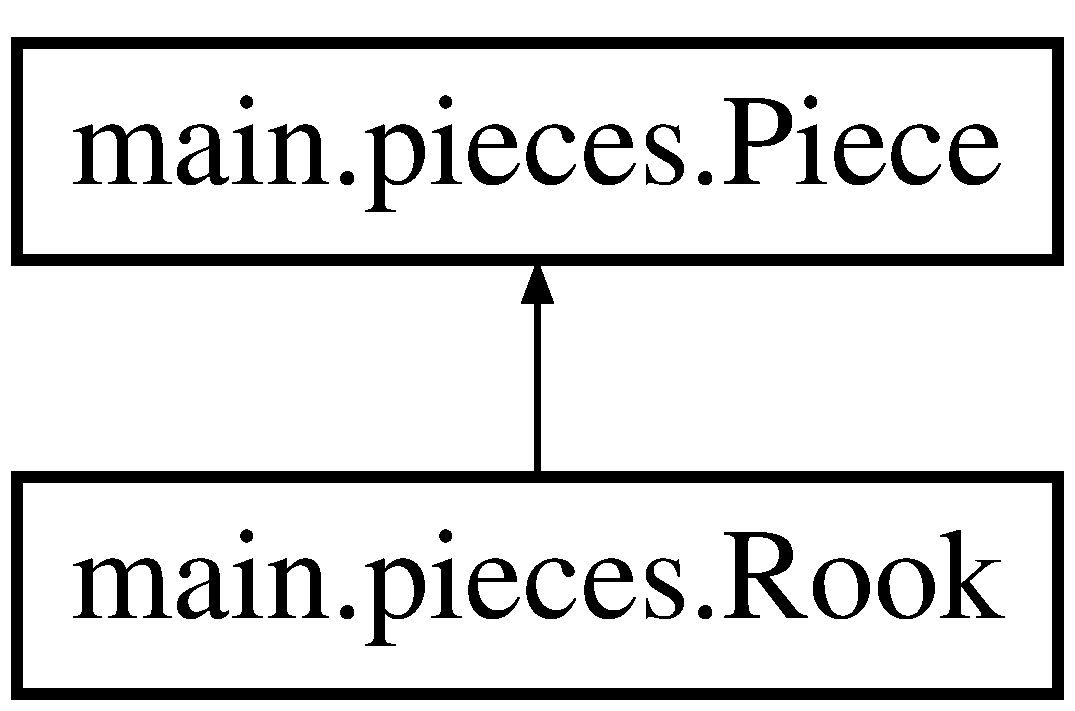
\includegraphics[height=2.000000cm]{classmain_1_1pieces_1_1_rook}
\end{center}
\end{figure}
\subsection*{Public Member Functions}
\begin{DoxyCompactItemize}
\item 
\hyperlink{classmain_1_1pieces_1_1_rook_af43778247abc01b02f8bd7f1bc7ecb17}{Rook} (String color)
\item 
String \hyperlink{classmain_1_1pieces_1_1_rook_aa92d82c81ad259daa0a3722e6bba870c}{get\+Type} ()
\item 
String \hyperlink{classmain_1_1pieces_1_1_rook_aa4408e34efd361045d25687da3103103}{to\+String} ()
\item 
Array\+List$<$ \hyperlink{classmain_1_1model_1_1_coordinate}{Coordinate} $>$ \hyperlink{classmain_1_1pieces_1_1_rook_acadd8cb22ffb2aef8ce68502b221a96e}{possible\+Moves} ()
\end{DoxyCompactItemize}
\subsection*{Additional Inherited Members}


\subsection{Detailed Description}
Created by samir on 9/2/16. 

\subsection{Constructor \& Destructor Documentation}
\hypertarget{classmain_1_1pieces_1_1_rook_af43778247abc01b02f8bd7f1bc7ecb17}{}\label{classmain_1_1pieces_1_1_rook_af43778247abc01b02f8bd7f1bc7ecb17} 
\index{main\+::pieces\+::\+Rook@{main\+::pieces\+::\+Rook}!Rook@{Rook}}
\index{Rook@{Rook}!main\+::pieces\+::\+Rook@{main\+::pieces\+::\+Rook}}
\subsubsection{\texorpdfstring{Rook()}{Rook()}}
{\footnotesize\ttfamily main.\+pieces.\+Rook.\+Rook (\begin{DoxyParamCaption}\item[{String}]{color }\end{DoxyParamCaption})}

Constructor taking in an x and y coordinate 

\subsection{Member Function Documentation}
\hypertarget{classmain_1_1pieces_1_1_rook_aa92d82c81ad259daa0a3722e6bba870c}{}\label{classmain_1_1pieces_1_1_rook_aa92d82c81ad259daa0a3722e6bba870c} 
\index{main\+::pieces\+::\+Rook@{main\+::pieces\+::\+Rook}!get\+Type@{get\+Type}}
\index{get\+Type@{get\+Type}!main\+::pieces\+::\+Rook@{main\+::pieces\+::\+Rook}}
\subsubsection{\texorpdfstring{get\+Type()}{getType()}}
{\footnotesize\ttfamily String main.\+pieces.\+Rook.\+get\+Type (\begin{DoxyParamCaption}{ }\end{DoxyParamCaption})}

Returns the type of this piece \hypertarget{classmain_1_1pieces_1_1_rook_acadd8cb22ffb2aef8ce68502b221a96e}{}\label{classmain_1_1pieces_1_1_rook_acadd8cb22ffb2aef8ce68502b221a96e} 
\index{main\+::pieces\+::\+Rook@{main\+::pieces\+::\+Rook}!possible\+Moves@{possible\+Moves}}
\index{possible\+Moves@{possible\+Moves}!main\+::pieces\+::\+Rook@{main\+::pieces\+::\+Rook}}
\subsubsection{\texorpdfstring{possible\+Moves()}{possibleMoves()}}
{\footnotesize\ttfamily Array\+List$<$\hyperlink{classmain_1_1model_1_1_coordinate}{Coordinate}$>$ main.\+pieces.\+Rook.\+possible\+Moves (\begin{DoxyParamCaption}{ }\end{DoxyParamCaption})}

\begin{DoxyReturn}{Returns}

\end{DoxyReturn}
\hypertarget{classmain_1_1pieces_1_1_rook_aa4408e34efd361045d25687da3103103}{}\label{classmain_1_1pieces_1_1_rook_aa4408e34efd361045d25687da3103103} 
\index{main\+::pieces\+::\+Rook@{main\+::pieces\+::\+Rook}!to\+String@{to\+String}}
\index{to\+String@{to\+String}!main\+::pieces\+::\+Rook@{main\+::pieces\+::\+Rook}}
\subsubsection{\texorpdfstring{to\+String()}{toString()}}
{\footnotesize\ttfamily String main.\+pieces.\+Rook.\+to\+String (\begin{DoxyParamCaption}{ }\end{DoxyParamCaption})}

String representation of a \hyperlink{classmain_1_1pieces_1_1_rook}{Rook} \begin{DoxyReturn}{Returns}

\end{DoxyReturn}


The documentation for this class was generated from the following file\+:\begin{DoxyCompactItemize}
\item 
src/main/pieces/Rook.\+java\end{DoxyCompactItemize}

\hypertarget{classtests_1_1pieces_1_1_rook_test}{}\section{tests.\+pieces.\+Rook\+Test Class Reference}
\label{classtests_1_1pieces_1_1_rook_test}\index{tests.\+pieces.\+Rook\+Test@{tests.\+pieces.\+Rook\+Test}}
\subsection*{Public Member Functions}
\begin{DoxyCompactItemize}
\item 
void \hyperlink{classtests_1_1pieces_1_1_rook_test_af9fc3b1f6a4fbc8e9312842ca0b8b595}{valid\+Rook\+Constructor} ()  throws Exception 
\item 
void \hyperlink{classtests_1_1pieces_1_1_rook_test_aca9621adf1a4fbe5911ab3b4b1edfee2}{valid\+Rook\+Movement} ()  throws Exception 
\end{DoxyCompactItemize}


\subsection{Detailed Description}
Created by samir on 9/5/16. 

\subsection{Member Function Documentation}
\hypertarget{classtests_1_1pieces_1_1_rook_test_af9fc3b1f6a4fbc8e9312842ca0b8b595}{}\label{classtests_1_1pieces_1_1_rook_test_af9fc3b1f6a4fbc8e9312842ca0b8b595} 
\index{tests\+::pieces\+::\+Rook\+Test@{tests\+::pieces\+::\+Rook\+Test}!valid\+Rook\+Constructor@{valid\+Rook\+Constructor}}
\index{valid\+Rook\+Constructor@{valid\+Rook\+Constructor}!tests\+::pieces\+::\+Rook\+Test@{tests\+::pieces\+::\+Rook\+Test}}
\subsubsection{\texorpdfstring{valid\+Rook\+Constructor()}{validRookConstructor()}}
{\footnotesize\ttfamily void tests.\+pieces.\+Rook\+Test.\+valid\+Rook\+Constructor (\begin{DoxyParamCaption}{ }\end{DoxyParamCaption}) throws Exception}

Valid constructor for a rook should not throw an exception \hypertarget{classtests_1_1pieces_1_1_rook_test_aca9621adf1a4fbe5911ab3b4b1edfee2}{}\label{classtests_1_1pieces_1_1_rook_test_aca9621adf1a4fbe5911ab3b4b1edfee2} 
\index{tests\+::pieces\+::\+Rook\+Test@{tests\+::pieces\+::\+Rook\+Test}!valid\+Rook\+Movement@{valid\+Rook\+Movement}}
\index{valid\+Rook\+Movement@{valid\+Rook\+Movement}!tests\+::pieces\+::\+Rook\+Test@{tests\+::pieces\+::\+Rook\+Test}}
\subsubsection{\texorpdfstring{valid\+Rook\+Movement()}{validRookMovement()}}
{\footnotesize\ttfamily void tests.\+pieces.\+Rook\+Test.\+valid\+Rook\+Movement (\begin{DoxyParamCaption}{ }\end{DoxyParamCaption}) throws Exception}

Test for valid rook movement (should be able to move) Check the valid moves match up 
\begin{DoxyExceptions}{Exceptions}
{\em Exception} & \\
\hline
\end{DoxyExceptions}


The documentation for this class was generated from the following file\+:\begin{DoxyCompactItemize}
\item 
src/tests/pieces/Rook\+Test.\+java\end{DoxyCompactItemize}

\hypertarget{classtests_1_1_run_all_tests}{}\section{tests.\+Run\+All\+Tests Class Reference}
\label{classtests_1_1_run_all_tests}\index{tests.\+Run\+All\+Tests@{tests.\+Run\+All\+Tests}}
Inheritance diagram for tests.\+Run\+All\+Tests\+:\begin{figure}[H]
\begin{center}
\leavevmode
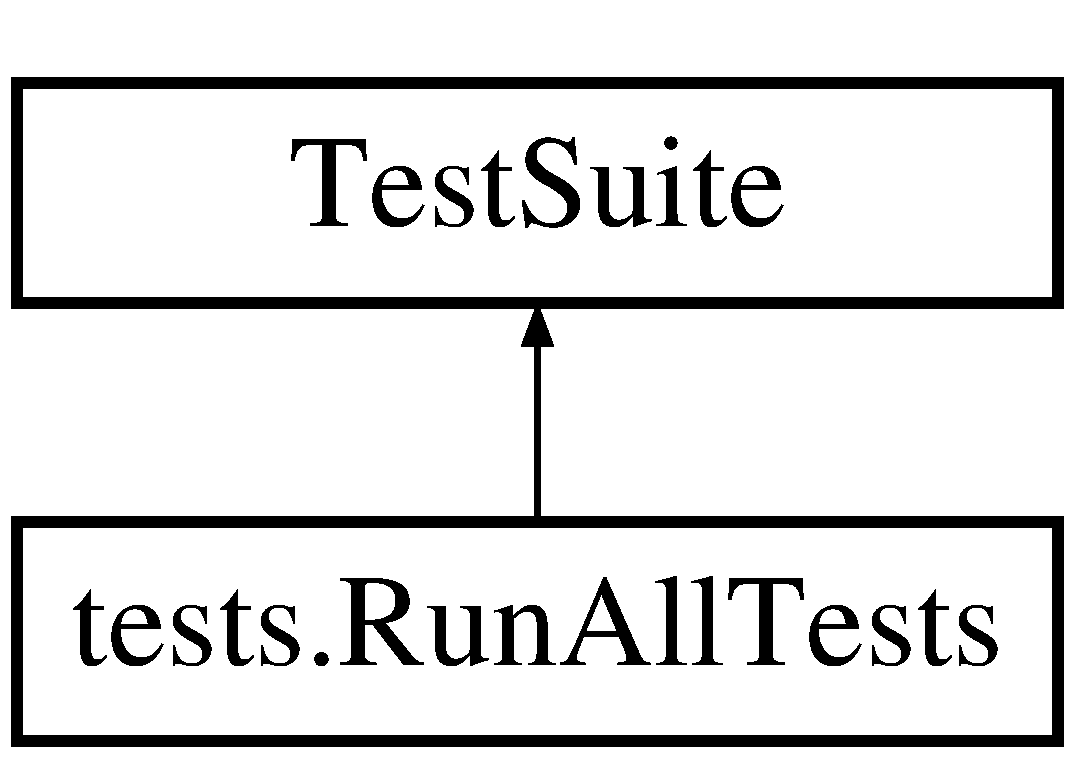
\includegraphics[height=2.000000cm]{classtests_1_1_run_all_tests}
\end{center}
\end{figure}


\subsection{Detailed Description}
Created by samir on 9/21/16. 

The documentation for this class was generated from the following file\+:\begin{DoxyCompactItemize}
\item 
src/tests/Run\+All\+Tests.\+java\end{DoxyCompactItemize}

%--- End generated contents ---

% Index
\backmatter
\newpage
\phantomsection
\clearemptydoublepage
\addcontentsline{toc}{chapter}{Index}
\printindex

\end{document}
